% Options for packages loaded elsewhere
\PassOptionsToPackage{unicode}{hyperref}
\PassOptionsToPackage{hyphens}{url}
\PassOptionsToPackage{dvipsnames,svgnames,x11names}{xcolor}
%
\documentclass[
  11pt,
  letterpaper,
  DIV=11,
  numbers=noendperiod]{scrreprt}

\usepackage{amsmath,amssymb}
\usepackage{iftex}
\ifPDFTeX
  \usepackage[T1]{fontenc}
  \usepackage[utf8]{inputenc}
  \usepackage{textcomp} % provide euro and other symbols
\else % if luatex or xetex
  \usepackage{unicode-math}
  \defaultfontfeatures{Scale=MatchLowercase}
  \defaultfontfeatures[\rmfamily]{Ligatures=TeX,Scale=1}
\fi
\usepackage[]{libertine}
\ifPDFTeX\else  
    % xetex/luatex font selection
\fi
% Use upquote if available, for straight quotes in verbatim environments
\IfFileExists{upquote.sty}{\usepackage{upquote}}{}
\IfFileExists{microtype.sty}{% use microtype if available
  \usepackage[]{microtype}
  \UseMicrotypeSet[protrusion]{basicmath} % disable protrusion for tt fonts
}{}
\makeatletter
\@ifundefined{KOMAClassName}{% if non-KOMA class
  \IfFileExists{parskip.sty}{%
    \usepackage{parskip}
  }{% else
    \setlength{\parindent}{0pt}
    \setlength{\parskip}{6pt plus 2pt minus 1pt}}
}{% if KOMA class
  \KOMAoptions{parskip=half}}
\makeatother
\usepackage{xcolor}
\usepackage[left=3cm,right=3cm,top=2cm,bottom=2cm,heightrounded]{geometry}
\setlength{\emergencystretch}{3em} % prevent overfull lines
\setcounter{secnumdepth}{5}
% Make \paragraph and \subparagraph free-standing
\ifx\paragraph\undefined\else
  \let\oldparagraph\paragraph
  \renewcommand{\paragraph}[1]{\oldparagraph{#1}\mbox{}}
\fi
\ifx\subparagraph\undefined\else
  \let\oldsubparagraph\subparagraph
  \renewcommand{\subparagraph}[1]{\oldsubparagraph{#1}\mbox{}}
\fi

\usepackage{color}
\usepackage{fancyvrb}
\newcommand{\VerbBar}{|}
\newcommand{\VERB}{\Verb[commandchars=\\\{\}]}
\DefineVerbatimEnvironment{Highlighting}{Verbatim}{commandchars=\\\{\}}
% Add ',fontsize=\small' for more characters per line
\usepackage{framed}
\definecolor{shadecolor}{RGB}{241,243,245}
\newenvironment{Shaded}{\begin{snugshade}}{\end{snugshade}}
\newcommand{\AlertTok}[1]{\textcolor[rgb]{0.68,0.00,0.00}{#1}}
\newcommand{\AnnotationTok}[1]{\textcolor[rgb]{0.37,0.37,0.37}{#1}}
\newcommand{\AttributeTok}[1]{\textcolor[rgb]{0.40,0.45,0.13}{#1}}
\newcommand{\BaseNTok}[1]{\textcolor[rgb]{0.68,0.00,0.00}{#1}}
\newcommand{\BuiltInTok}[1]{\textcolor[rgb]{0.00,0.23,0.31}{#1}}
\newcommand{\CharTok}[1]{\textcolor[rgb]{0.13,0.47,0.30}{#1}}
\newcommand{\CommentTok}[1]{\textcolor[rgb]{0.37,0.37,0.37}{#1}}
\newcommand{\CommentVarTok}[1]{\textcolor[rgb]{0.37,0.37,0.37}{\textit{#1}}}
\newcommand{\ConstantTok}[1]{\textcolor[rgb]{0.56,0.35,0.01}{#1}}
\newcommand{\ControlFlowTok}[1]{\textcolor[rgb]{0.00,0.23,0.31}{#1}}
\newcommand{\DataTypeTok}[1]{\textcolor[rgb]{0.68,0.00,0.00}{#1}}
\newcommand{\DecValTok}[1]{\textcolor[rgb]{0.68,0.00,0.00}{#1}}
\newcommand{\DocumentationTok}[1]{\textcolor[rgb]{0.37,0.37,0.37}{\textit{#1}}}
\newcommand{\ErrorTok}[1]{\textcolor[rgb]{0.68,0.00,0.00}{#1}}
\newcommand{\ExtensionTok}[1]{\textcolor[rgb]{0.00,0.23,0.31}{#1}}
\newcommand{\FloatTok}[1]{\textcolor[rgb]{0.68,0.00,0.00}{#1}}
\newcommand{\FunctionTok}[1]{\textcolor[rgb]{0.28,0.35,0.67}{#1}}
\newcommand{\ImportTok}[1]{\textcolor[rgb]{0.00,0.46,0.62}{#1}}
\newcommand{\InformationTok}[1]{\textcolor[rgb]{0.37,0.37,0.37}{#1}}
\newcommand{\KeywordTok}[1]{\textcolor[rgb]{0.00,0.23,0.31}{#1}}
\newcommand{\NormalTok}[1]{\textcolor[rgb]{0.00,0.23,0.31}{#1}}
\newcommand{\OperatorTok}[1]{\textcolor[rgb]{0.37,0.37,0.37}{#1}}
\newcommand{\OtherTok}[1]{\textcolor[rgb]{0.00,0.23,0.31}{#1}}
\newcommand{\PreprocessorTok}[1]{\textcolor[rgb]{0.68,0.00,0.00}{#1}}
\newcommand{\RegionMarkerTok}[1]{\textcolor[rgb]{0.00,0.23,0.31}{#1}}
\newcommand{\SpecialCharTok}[1]{\textcolor[rgb]{0.37,0.37,0.37}{#1}}
\newcommand{\SpecialStringTok}[1]{\textcolor[rgb]{0.13,0.47,0.30}{#1}}
\newcommand{\StringTok}[1]{\textcolor[rgb]{0.13,0.47,0.30}{#1}}
\newcommand{\VariableTok}[1]{\textcolor[rgb]{0.07,0.07,0.07}{#1}}
\newcommand{\VerbatimStringTok}[1]{\textcolor[rgb]{0.13,0.47,0.30}{#1}}
\newcommand{\WarningTok}[1]{\textcolor[rgb]{0.37,0.37,0.37}{\textit{#1}}}

\providecommand{\tightlist}{%
  \setlength{\itemsep}{0pt}\setlength{\parskip}{0pt}}\usepackage{longtable,booktabs,array}
\usepackage{calc} % for calculating minipage widths
% Correct order of tables after \paragraph or \subparagraph
\usepackage{etoolbox}
\makeatletter
\patchcmd\longtable{\par}{\if@noskipsec\mbox{}\fi\par}{}{}
\makeatother
% Allow footnotes in longtable head/foot
\IfFileExists{footnotehyper.sty}{\usepackage{footnotehyper}}{\usepackage{footnote}}
\makesavenoteenv{longtable}
\usepackage{graphicx}
\makeatletter
\def\maxwidth{\ifdim\Gin@nat@width>\linewidth\linewidth\else\Gin@nat@width\fi}
\def\maxheight{\ifdim\Gin@nat@height>\textheight\textheight\else\Gin@nat@height\fi}
\makeatother
% Scale images if necessary, so that they will not overflow the page
% margins by default, and it is still possible to overwrite the defaults
% using explicit options in \includegraphics[width, height, ...]{}
\setkeys{Gin}{width=\maxwidth,height=\maxheight,keepaspectratio}
% Set default figure placement to htbp
\makeatletter
\def\fps@figure{htbp}
\makeatother
% definitions for citeproc citations
\NewDocumentCommand\citeproctext{}{}
\NewDocumentCommand\citeproc{mm}{%
  \begingroup\def\citeproctext{#2}\cite{#1}\endgroup}
\makeatletter
 % allow citations to break across lines
 \let\@cite@ofmt\@firstofone
 % avoid brackets around text for \cite:
 \def\@biblabel#1{}
 \def\@cite#1#2{{#1\if@tempswa , #2\fi}}
\makeatother
\newlength{\cslhangindent}
\setlength{\cslhangindent}{1.5em}
\newlength{\csllabelwidth}
\setlength{\csllabelwidth}{3em}
\newenvironment{CSLReferences}[2] % #1 hanging-indent, #2 entry-spacing
 {\begin{list}{}{%
  \setlength{\itemindent}{0pt}
  \setlength{\leftmargin}{0pt}
  \setlength{\parsep}{0pt}
  % turn on hanging indent if param 1 is 1
  \ifodd #1
   \setlength{\leftmargin}{\cslhangindent}
   \setlength{\itemindent}{-1\cslhangindent}
  \fi
  % set entry spacing
  \setlength{\itemsep}{#2\baselineskip}}}
 {\end{list}}
\usepackage{calc}
\newcommand{\CSLBlock}[1]{\hfill\break\parbox[t]{\linewidth}{\strut\ignorespaces#1\strut}}
\newcommand{\CSLLeftMargin}[1]{\parbox[t]{\csllabelwidth}{\strut#1\strut}}
\newcommand{\CSLRightInline}[1]{\parbox[t]{\linewidth - \csllabelwidth}{\strut#1\strut}}
\newcommand{\CSLIndent}[1]{\hspace{\cslhangindent}#1}

\KOMAoption{captions}{tableheading}
\usepackage{fancyhdr}
\pagestyle{fancy}
\fancyhf{}
\fancyhead[L]{\leftmark}
\fancyhead[R]{\thepage}
\fancyfoot[C]{Quantitative methods in corpus linguistics}
\makeatletter
\@ifpackageloaded{tcolorbox}{}{\usepackage[skins,breakable]{tcolorbox}}
\@ifpackageloaded{fontawesome5}{}{\usepackage{fontawesome5}}
\definecolor{quarto-callout-color}{HTML}{909090}
\definecolor{quarto-callout-note-color}{HTML}{0758E5}
\definecolor{quarto-callout-important-color}{HTML}{CC1914}
\definecolor{quarto-callout-warning-color}{HTML}{EB9113}
\definecolor{quarto-callout-tip-color}{HTML}{00A047}
\definecolor{quarto-callout-caution-color}{HTML}{FC5300}
\definecolor{quarto-callout-color-frame}{HTML}{acacac}
\definecolor{quarto-callout-note-color-frame}{HTML}{4582ec}
\definecolor{quarto-callout-important-color-frame}{HTML}{d9534f}
\definecolor{quarto-callout-warning-color-frame}{HTML}{f0ad4e}
\definecolor{quarto-callout-tip-color-frame}{HTML}{02b875}
\definecolor{quarto-callout-caution-color-frame}{HTML}{fd7e14}
\makeatother
\makeatletter
\@ifpackageloaded{caption}{}{\usepackage{caption}}
\AtBeginDocument{%
\ifdefined\contentsname
  \renewcommand*\contentsname{Table of contents}
\else
  \newcommand\contentsname{Table of contents}
\fi
\ifdefined\listfigurename
  \renewcommand*\listfigurename{List of Figures}
\else
  \newcommand\listfigurename{List of Figures}
\fi
\ifdefined\listtablename
  \renewcommand*\listtablename{List of Tables}
\else
  \newcommand\listtablename{List of Tables}
\fi
\ifdefined\figurename
  \renewcommand*\figurename{Figure}
\else
  \newcommand\figurename{Figure}
\fi
\ifdefined\tablename
  \renewcommand*\tablename{Table}
\else
  \newcommand\tablename{Table}
\fi
}
\@ifpackageloaded{float}{}{\usepackage{float}}
\floatstyle{ruled}
\@ifundefined{c@chapter}{\newfloat{codelisting}{h}{lop}}{\newfloat{codelisting}{h}{lop}[chapter]}
\floatname{codelisting}{Listing}
\newcommand*\listoflistings{\listof{codelisting}{List of Listings}}
\makeatother
\makeatletter
\makeatother
\makeatletter
\@ifpackageloaded{caption}{}{\usepackage{caption}}
\@ifpackageloaded{subcaption}{}{\usepackage{subcaption}}
\makeatother
\ifLuaTeX
  \usepackage{selnolig}  % disable illegal ligatures
\fi
\IfFileExists{bookmark.sty}{\usepackage{bookmark}}{\usepackage{hyperref}}
\IfFileExists{xurl.sty}{\usepackage{xurl}}{} % add URL line breaks if available
\urlstyle{same} % disable monospaced font for URLs
\hypersetup{
  pdftitle={Statistics and Data Analysis for Corpus Linguists: From Theory to Practice with R},
  pdfauthor={Vladimir Buskin},
  colorlinks=true,
  linkcolor={blue},
  filecolor={Maroon},
  citecolor={Blue},
  urlcolor={Blue},
  pdfcreator={LaTeX via pandoc}}

\title{Statistics and Data Analysis for Corpus Linguists: From Theory to
Practice with R}
\author{Vladimir Buskin}
\date{2024-06-30}

\begin{document}
\maketitle
\renewcommand*\contentsname{Table of contents}
{
\hypersetup{linkcolor=}
\setcounter{tocdepth}{2}
\tableofcontents
}
\chapter*{Preface}\label{preface}
\addcontentsline{toc}{chapter}{Preface}

\markboth{Preface}{Preface}

This collection of handouts provides a hands-on introduction to data
analysis and statistical methods in quantitative corpus linguistics with
R. It is designed with accessibility in mind, assuming no prior
knowledge of programming or statistics. All you need to get started is a
laptop; everything else will be explained within these pages.

Primarily, this reader is geared towards students attending the classes
\textbf{Language Variation} (BA) and \textbf{Statistics for Linguistics}
(MA) at the Catholic University of Eichstätt-Ingolstadt (Germany).
However, it is also meant to equip students currently working on their
\textbf{BA/MA/PhD theses} with the tools they need to conduct empirical
studies on a wide array of linguistic phenomena. The methods presented
here reflect the state-of-the-art in corpus-linguistic research,
providing readers with current and relevant analytical techniques.

\section*{Overview}\label{overview}
\addcontentsline{toc}{section}{Overview}

\markright{Overview}

We begin by establishing the general structure of corpus-linguistic
studies, accompanied by key theoretical and practical considerations.
The second section introduces R as an analytical tool, covering its core
functionality. With these fundamentals in place, we proceed to query
corpora directly within R. Chapters four and five focus on describing
discrete and continuous outputs, as well as identifying meaningful
associations and differences in the data (\textbf{BA}). Finally, to gain
more nuanced insights into potential patterns, we apply common machine
learning algorithms to fit, evaluate, and interpret statistical models
(\textbf{MA}).

Throughout this journey, readers will develop the skills to conduct
robust corpus-linguistic analyses, from basic querying to advanced
statistical modeling.

\part{Conducting a corpus-linguistic study}

\chapter{An example from
sociolinguistics}\label{an-example-from-sociolinguistics}

\section{Barbieri (2007): Older Men and Younger
Women}\label{barbierioldermenyounger2007-older-men-and-younger-women}

\subsection{Defining the Variable}\label{defining-the-variable}

New quotatives in American English: \emph{be like}, \emph{go}, \emph{be
all}:

\begin{enumerate}
\def\labelenumi{(\arabic{enumi})}
\tightlist
\item
  ``\emph{I was like} `well if it's not leaking, I don't care.'\,''
\item
  ``Do you, I asked I was running out and I \emph{go}, `you're trying to
  deliver a pizza here?'\,''
\item
  ``My sister's \emph{all} `excuse me would you mind if I gave you, if I
  want your autograph.'\,''
\end{enumerate}

\begin{tcolorbox}[enhanced jigsaw, toprule=.15mm, opacitybacktitle=0.6, coltitle=black, arc=.35mm, colback=white, title=\textcolor{quarto-callout-caution-color}{\faFire}\hspace{0.5em}{Task}, titlerule=0mm, toptitle=1mm, bottomtitle=1mm, breakable, rightrule=.15mm, opacityback=0, bottomrule=.15mm, leftrule=.75mm, colframe=quarto-callout-caution-color-frame, left=2mm, colbacktitle=quarto-callout-caution-color!10!white]

As you read through the following sections, think about \textbf{what
might go wrong} at each stage of the study!

\end{tcolorbox}

\subsection{Reviewing Previous
Research}\label{reviewing-previous-research}

\begin{itemize}
\tightlist
\item
  Previous results with regard to \textbf{age}: \emph{Be like} is known
  to be preferred by \textbf{younger speakers}.
\item
  Previous results with regard to \textbf{sex} are
  \textbf{inconclusive}.
\end{itemize}

\subsection{Research Question}\label{research-question}

\begin{quote}
``The study aims to contribute to the investigation of the controversial
question of the effect of \textbf{speaker's age} and \textbf{sex} on
quotative use in American English, focusing on the newer quotatives
\emph{be like}, \emph{go}, \emph{be all}'' (Barbieri 2007: 26).
\end{quote}

\subsection{Data}\label{data}

\begin{itemize}
\tightlist
\item
  \textbf{Choice of corpus}: 450,000 words taken from the Conversation
  component of the \emph{Longman Spoken and Written English Corpus} (all
  files where the age and gender of speakers were available), i.e.,
  about 50 hours of casual conversation coded for speakers' \textbf{age}
  and \textbf{sex}.
\item
  \textbf{Data extraction}: All forms of \emph{be like}, \emph{be all},
  \emph{go}, \emph{say} extracted using corpus linguistic software; data
  entered into spreadsheet software; word counts of texts added via
  Delphi program.
\end{itemize}

\subsection{Presentation of Results}\label{presentation-of-results}

\begin{longtable}[]{@{}
  >{\raggedright\arraybackslash}p{(\columnwidth - 6\tabcolsep) * \real{0.1944}}
  >{\raggedright\arraybackslash}p{(\columnwidth - 6\tabcolsep) * \real{0.1944}}
  >{\raggedright\arraybackslash}p{(\columnwidth - 6\tabcolsep) * \real{0.2917}}
  >{\raggedright\arraybackslash}p{(\columnwidth - 6\tabcolsep) * \real{0.3194}}@{}}
\toprule\noalign{}
\begin{minipage}[b]{\linewidth}\raggedright
Quotative
\end{minipage} & \begin{minipage}[b]{\linewidth}\raggedright
Age group
\end{minipage} & \begin{minipage}[b]{\linewidth}\raggedright
Male use (per 100,000 words)
\end{minipage} & \begin{minipage}[b]{\linewidth}\raggedright
Female use (per 100,000 words)
\end{minipage} \\
\midrule\noalign{}
\endhead
\bottomrule\noalign{}
\endlastfoot
\textbf{say} & 16--26 & 115 & 149 \\
& 27--40 & 101 & 117 \\
& 41--54 & 55 & 214 \\
& 55+ & 67 & 433 \\
\textbf{be like} & 16--26 & 32 & 329 \\
& 27--40 & 66 & 25 \\
& 41--54 & - & 1 \\
& 55+ & - & 19 \\
\textbf{go} & 16--26 & 25 & 113 \\
& 27--40 & 61 & 18 \\
& 41--54 & - & 15 \\
& 55+ & - & 7 \\
\textbf{be all} & 16--26 & 14 & 33 \\
\end{longtable}

\begin{figure}[H]

{\centering 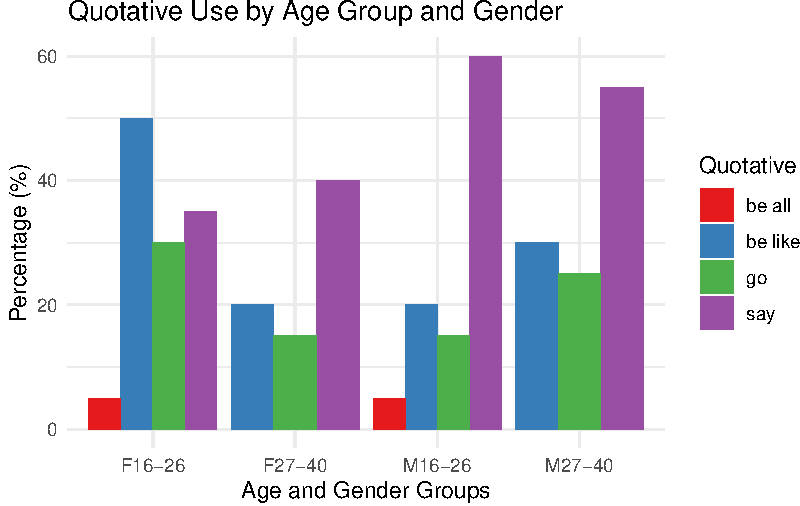
\includegraphics{Basics_files/figure-pdf/unnamed-chunk-1-1.pdf}

}

\caption{Reproduction of Barbieri's Figure 5 `Proportional quotative use
by men and women aged 16--26 and 27--40'}

\end{figure}%

\subsection{Formulation of Results}\label{formulation-of-results}

\begin{quote}
``In sum, the patterns of proportional use and the results of the
statistical analyses show that there are striking differences in the way
that men and women under the age of forty use quotative verbs. In
contrast, in conforming to the traditional quotative \emph{say}, men and
women over forty displayed similar behavior'' (Barbieri 2007: 38--39).
\end{quote}

\subsection{Some of her conclusions}\label{some-of-her-conclusions}

\begin{quote}
``In favoring \emph{be like} over other quotatives, men in their late
20s and in their 30s display an `affinity' with slightly younger women,
women in their early 20s, rather than with women of their same age''
(Barbieri 2007: 41).
\end{quote}

\section{Principles of Empirical
Linguistics}\label{principles-of-empirical-linguistics}

\begin{itemize}
\item
  \textbf{Objectivity} --- Independence from researchers or devices (→
  replicability!)
\item
  \textbf{Reliability} --- Studies should be replicable.
\item
  \textbf{Validity} --- A study must actually address the problem
  formulated in the research question.
\end{itemize}

\chapter{Research questions}\label{research-questions}

\section{What makes a good research
question?}\label{what-makes-a-good-research-question}

\subsection{The structure of research
questions}\label{the-structure-of-research-questions}

\textbf{Example}: I am studying the pronunciation of {[}r{]} in New York
because I want to find out whether different social groups differ with
respect to their pronunciation, in order to help my readers understand
how social factors influence our linguistic behavior.

\begin{enumerate}
\def\labelenumi{\arabic{enumi}.}
\item
  \textbf{Topic}: \texttt{I\ am\ studying...}
\item
  \textbf{Indirect question}:
  \texttt{Because\ I\ want\ to\ find\ out\ what,\ why,\ how...}
\item
  \textbf{(General) linguistic significance}:
  \texttt{...\ in\ order\ to\ help\ the\ readers\ understand\ how,\ why,\ or\ whether...}
\end{enumerate}

\begin{quote}
Cf. Booth, Colomb, and Williams (2008): 45--48
\end{quote}

\begin{tcolorbox}[enhanced jigsaw, toprule=.15mm, opacitybacktitle=0.6, coltitle=black, arc=.35mm, colback=white, title=\textcolor{quarto-callout-caution-color}{\faFire}\hspace{0.5em}{Task}, titlerule=0mm, toptitle=1mm, bottomtitle=1mm, breakable, rightrule=.15mm, opacityback=0, bottomrule=.15mm, leftrule=.75mm, colframe=quarto-callout-caution-color-frame, left=2mm, colbacktitle=quarto-callout-caution-color!10!white]

Assess the following research questions!

\begin{enumerate}
\def\labelenumi{(\alph{enumi})}
\item
  I will try to find the specific linguistic features which a Shetlander
  uses when speaking Scottish standard English, i.e., Shetland accent in
  Scottish Standard English.
\item
  In this paper, I am going to analyze the use of American and Indian
  dialect features among Indian immigrants to the US because I want to
  find out whether they correlate with their willingness to integrate
  into American society; this will show the degree to which linguistic
  adaptation depends on cultural orientation.
\item
  In this paper, I am going to address the question of how gender
  influences language.
\item
  The study aims to contribute to the investigation of the controversial
  question of the effect of speaker's age and sex on quotative use in
  American English, focusing on the newer quotatives \emph{be like},
  \emph{go}, \emph{be all}.
\item
  In this paper, adverts by Coca-Cola and Pepsi will be analyzed for the
  use of verb forms.
\end{enumerate}

\end{tcolorbox}

\subsection{Hints for good research
questions}\label{hints-for-good-research-questions}

\begin{tcolorbox}[enhanced jigsaw, toprule=.15mm, opacitybacktitle=0.6, coltitle=black, arc=.35mm, colback=white, title=\textcolor{quarto-callout-tip-color}{\faLightbulb}\hspace{0.5em}{Tip}, titlerule=0mm, toptitle=1mm, bottomtitle=1mm, breakable, rightrule=.15mm, opacityback=0, bottomrule=.15mm, leftrule=.75mm, colframe=quarto-callout-tip-color-frame, left=2mm, colbacktitle=quarto-callout-tip-color!10!white]

\begin{enumerate}
\def\labelenumi{\arabic{enumi}.}
\item
  A research question must be \textbf{simple, specific, and doable}. It
  is better to make a small contribution to a particular problem than to
  aim at covering a whole subfield of sociolinguistics.
\item
  Keep a research question \textbf{stable} in your paper, even if you
  come across interesting new ideas as you work on it.
\item
  The research question must be an \textbf{explicit part of your paper}.
  Mention it in the introduction and keep referring back to it from time
  to time.
\item
  Keep in mind that the research question will determine both
  \textbf{methodology} and \textbf{data}.
\end{enumerate}

\begin{quote}
Cf. Hazen (2015): 9--10
\end{quote}

\end{tcolorbox}

\subsection{Hypotheses}\label{hypotheses}

Research questions must be complemented by a set of falsifiable
hypotheses. These are covered in-depth under
\texttt{Inferential\ statistics\ \textgreater{}\ Hypothesis\ testing}.
In short,

\begin{itemize}
\item
  \textbf{Hypothesis H}1 predicts a specific relationship between a
  dependent variable and an independent variable.
\item
  its \textbf{opposite}, \textbf{Hypothesis H}0, describes the state of
  affairs where the predicted relationship between the variables does
  not hold.
\end{itemize}

The predictions made by the hypotheses are based on previous research.
Here is an example:

\textbf{Research question}: I am studying the pronunciation of {[}r{]}
in New York because I want to find out whether different social groups
differ with respect to their pronunciation, in order to help my readers
understand how social factors influence our linguistic behavior.

\begin{itemize}
\item
  \textbf{Hypothesis H}1: Upper-class speakers will use postvocalic /r/
  more frequently than lower-class speakers.
\item
  \textbf{Hypothesis H}0: Upper-class speakers will \textbf{not} use
  postvocalic /r/ more frequently than lower-class speakers.
\end{itemize}

\subsection{Practice}\label{practice}

\textbf{Task}: Develop valid research questions on the basis of the
following linguistic variables:

\begin{enumerate}
\def\labelenumi{\arabic{enumi}.}
\item
  Speakers in bilingual conversations are especially likely to
  code-switch when there is a significant change of topic.
\item
  Women use more tentative language in conversations than men.
\end{enumerate}

\chapter{Linguistic variables}\label{linguistic-variables}

\section{What is a linguistic
variable?}\label{what-is-a-linguistic-variable}

\begin{enumerate}
\def\labelenumi{\arabic{enumi}.}
\item
  \textbf{The classical view:} Labov (1972) defines a linguistic
  variable as ``two ways of saying the same thing.''
\item
  \textbf{A restriction:} Meyerhoff (2009, p.~11) summarized, ``In sum,
  a sociolinguistic variable can be defined as a linguistic variable
  that is constrained by social or non-linguistic factors\ldots{}''
\item
  \textbf{A more open view:} Kiesling (2011) argued, ``Given the
  variability of what counts as a variable, we must define what counts
  as a variable more broadly than `two or more ways of saying the same
  thing'. We will simply say that a linguistic variable is a choice or
  option about speaking in a speech community\ldots{} Note that this
  definition does not in any way require us to state that the meaning be
  the same, although there should be some kind of equivalence noted.''
\end{enumerate}

\begin{tcolorbox}[enhanced jigsaw, toprule=.15mm, opacitybacktitle=0.6, coltitle=black, arc=.35mm, colback=white, title=\textcolor{quarto-callout-caution-color}{\faFire}\hspace{0.5em}{Discussion}, titlerule=0mm, toptitle=1mm, bottomtitle=1mm, breakable, rightrule=.15mm, opacityback=0, bottomrule=.15mm, leftrule=.75mm, colframe=quarto-callout-caution-color-frame, left=2mm, colbacktitle=quarto-callout-caution-color!10!white]

Which of the following variables are good sociolinguistic variables, and
which of them are poor?

\begin{enumerate}
\def\labelenumi{\arabic{enumi}.}
\tightlist
\item
  /fɔːθ flɔː/ vs.~/fɔːrθ flɔːr/
\item
  \emph{This enables him to preside over the process which I have
  described} vs.~\emph{This enables him to preside over the process that
  I have described} vs.~\emph{This enables him to preside over the
  process ∅ I have described}.
\item
  \emph{The pair found the briefcase on a bus station bench at Bath
  central bus station.} vs.~\emph{The briefcase was found on a bus
  station bench at Bath central bus station by the pair.}
\item
  \emph{Art is after all the subject of attention for both critic and
  historian, even though the functions and methods of the two sorts of
  writer have drawn apart.} vs.~\emph{Art histories often make an
  attempt to keep to chronology, although the difficulties include the
  crucial fact that in art there is no clear sequence of events.}
  vs.~\emph{Many of his readers approved his sensitive and appreciative
  understanding of paintings, though without sharing his political
  views.}
\item
  /pleɪŋ/ vs.~/pleɪn/
\item
  {[}tʰ{]} in /tɔp/ vs.~{[}t{]} in \emph{stop}.
\end{enumerate}

\end{tcolorbox}

\section{The principle of
accountability}\label{the-principle-of-accountability}

\begin{tcolorbox}[enhanced jigsaw, toprule=.15mm, opacitybacktitle=0.6, coltitle=black, arc=.35mm, colback=white, title=\textcolor{quarto-callout-caution-color}{\faFire}\hspace{0.5em}{Task}, titlerule=0mm, toptitle=1mm, bottomtitle=1mm, breakable, rightrule=.15mm, opacityback=0, bottomrule=.15mm, leftrule=.75mm, colframe=quarto-callout-caution-color-frame, left=2mm, colbacktitle=quarto-callout-caution-color!10!white]

Two linguists aim to study the preference for passives among men and
women. They extract all the passives from 500,000 words of male speech
and all passives from 500,000 words of female speech and report the
results. \textbf{What's wrong?}

\end{tcolorbox}

\section{Subtypes of variables}\label{subtypes-of-variables}

\subsection{Linguistic perspective}\label{linguistic-perspective}

\begin{enumerate}
\def\labelenumi{\arabic{enumi}.}
\tightlist
\item
  phonetic/phonological
\item
  morphological
\item
  syntactic
\item
  pragmatic
\end{enumerate}

\subsection{Sociolinguistic
perspective}\label{sociolinguistic-perspective}

Sociolinguistic variables also differ with regard to their
\textbf{salience} in society.

\begin{enumerate}
\def\labelenumi{\arabic{enumi}.}
\tightlist
\item
  \textbf{Stereotypes} are strongly socially marked and part of popular
  discourse about language.

  \begin{itemize}
  \tightlist
  \item
    \emph{h}-dropping in Cockney
  \item
    Canadian \emph{eh} at the end of sentences
  \item
    Australian \emph{dinkum}: \emph{I was fair dinkum about my interest
    in their culture} `authentic, genuine'
  \end{itemize}
\item
  \textbf{Markers} show both social and style stratification; all
  members of a society react similarly in taking care to \textbf{avoid
  the pattern} in \textbf{formal registers}.

  \begin{itemize}
  \item
    \begin{enumerate}
    \def\labelenumii{(\alph{enumii})}
    \setcounter{enumii}{17}
    \tightlist
    \item
    \end{enumerate}
  \item
    (th)
  \end{itemize}
\item
  \textbf{Indicators} differentiate social groups. However, people are
  not aware of them and therefore do not avoid them in formal registers.

  \begin{itemize}
  \tightlist
  \item
    Same vowel in \emph{God} and \emph{Guard} in New York City
  \end{itemize}
\end{enumerate}

\begin{quote}
Taken from Mesthrie, Rajend, et al.~\emph{Introducing Sociolinguistics}.
Edinburgh University Press, 2009.
\end{quote}

\section{Statistical perspective}\label{statistical-perspective}

\subsection{Dependent and independent
variables}\label{dependent-and-independent-variables}

\textbf{Task:} Decide which of the variables are \textbf{independent},
and which are \textbf{dependent variables}!

\begin{longtable}[]{@{}lll@{}}
\toprule\noalign{}
& Kenyan speakers & Singaporean speakers \\
\midrule\noalign{}
\endhead
\bottomrule\noalign{}
\endlastfoot
Average sentence length & 10.5 & 9.8 \\
\end{longtable}

\begin{longtable}[]{@{}lll@{}}
\toprule\noalign{}
& male & female \\
\midrule\noalign{}
\endhead
\bottomrule\noalign{}
\endlastfoot
\emph{actually} & 65 & 98 \\
\emph{possibly} & 55 & 77 \\
\emph{really} & 54 & 55 \\
\end{longtable}

\begin{longtable}[]{@{}
  >{\raggedright\arraybackslash}p{(\columnwidth - 10\tabcolsep) * \real{0.2958}}
  >{\raggedright\arraybackslash}p{(\columnwidth - 10\tabcolsep) * \real{0.1408}}
  >{\raggedright\arraybackslash}p{(\columnwidth - 10\tabcolsep) * \real{0.1408}}
  >{\raggedright\arraybackslash}p{(\columnwidth - 10\tabcolsep) * \real{0.1408}}
  >{\raggedright\arraybackslash}p{(\columnwidth - 10\tabcolsep) * \real{0.1408}}
  >{\raggedright\arraybackslash}p{(\columnwidth - 10\tabcolsep) * \real{0.1408}}@{}}
\toprule\noalign{}
\begin{minipage}[b]{\linewidth}\raggedright
Question: English is the most important language today.
\end{minipage} & \begin{minipage}[b]{\linewidth}\raggedright
\textbf{strongly agree}
\end{minipage} & \begin{minipage}[b]{\linewidth}\raggedright
\textbf{agree}
\end{minipage} & \begin{minipage}[b]{\linewidth}\raggedright
\textbf{neutral}
\end{minipage} & \begin{minipage}[b]{\linewidth}\raggedright
\textbf{disagree}
\end{minipage} & \begin{minipage}[b]{\linewidth}\raggedright
\textbf{strongly disagree}
\end{minipage} \\
\midrule\noalign{}
\endhead
\bottomrule\noalign{}
\endlastfoot
N & 12 & 33 & 58 & 12 & 8 \\
\end{longtable}

\subsection{Interval, ordinal, and
nominal}\label{interval-ordinal-and-nominal}

\begin{enumerate}
\def\labelenumi{\arabic{enumi}.}
\tightlist
\item
  COMPLEXITY (ordinal)

  \begin{itemize}
  \tightlist
  \item
    \emph{the book} (low)
  \item
    \emph{the brown book} (middle)
  \item
    \emph{the book I had bought in Europe} (high)
  \end{itemize}
\item
  LENGTH (interval)

  \begin{itemize}
  \tightlist
  \item
    \emph{book} (1)
  \item
    \emph{the book} (2)
  \item
    \emph{the book I had bought in Europe} (7)
  \end{itemize}
\item
  ANIMACY (nominal)

  \begin{itemize}
  \tightlist
  \item
    \emph{He picked up \textbf{the book}.}
  \item
    \emph{He picked \textbf{his dad} up.}
  \end{itemize}
\end{enumerate}

\begin{quote}
Cf. Gries, Stefan Th. \emph{Statistics for Linguistics with R}. De
Gruyter Mouton, 2013, p.~9.
\end{quote}

\textbf{Task:} Now, go back to Tables 1--3 and decide which of the
variables are \textbf{interval variables}, \textbf{ordinal} or
\textbf{nominal} variables!

\section{Many morphosyntactic variables in
English}\label{many-morphosyntactic-variables-in-english}

\begin{longtable}[]{@{}
  >{\raggedright\arraybackslash}p{(\columnwidth - 2\tabcolsep) * \real{0.4444}}
  >{\raggedright\arraybackslash}p{(\columnwidth - 2\tabcolsep) * \real{0.5556}}@{}}
\toprule\noalign{}
\begin{minipage}[b]{\linewidth}\raggedright
Variable
\end{minipage} & \begin{minipage}[b]{\linewidth}\raggedright
Example
\end{minipage} \\
\midrule\noalign{}
\endhead
\bottomrule\noalign{}
\endlastfoot
Indefinite Pronouns & \emph{everybody} vs.~\emph{everyone} \\
Case and order of coordinated pronouns & \emph{my husband and I}
vs.~\emph{my husband and me} vs.~\emph{me and my husband} \\
\emph{that} vs.~zero complementation & \emph{I don't think
\textbf{that}/Ø it's a problem.} \\
\emph{that} vs.~gerundial complementation & \emph{remember
\textbf{that}} vs.~\emph{remember \textbf{V-ing}}; \emph{try to}
vs.~\emph{try and} vs.~\emph{try V-ing} \\
Particle placement & \emph{set the computer up} vs.~\emph{set up the
computer} \\
The dative alternation & \emph{give the book to John} vs.~\emph{give
John the book} \\
The genitive alternation & \emph{John's house} vs.~\emph{the house of
John} \\
Relativization strategies & \emph{wh}-word vs.~\emph{that} vs.~Ø \\
Analytic vs.~synthetic comparatives & \emph{warmer} vs.~\emph{more
scary} \\
Plural existentials & \emph{there are some places} vs.~\emph{there's
some places} \\
Future temporal reference & \emph{will} vs.~\emph{going to}
vs.~progressive etc. \\
Deontic modality & \emph{must} vs.~\emph{have to} vs.~\emph{need to}
vs.~\emph{got to} etc. \\
Stative possession & \emph{have} vs.~\emph{have got} vs.~\emph{got} \\
Quotatives & \emph{say} vs.~\emph{be like} vs.~\emph{go} etc. \\
\emph{not} vs.~\emph{no} & \emph{not anybody} vs.~\emph{nobody};
\emph{not anyone} vs.~\emph{no one}; \emph{not anything}
vs.~\emph{nothing} \\
\emph{NOT} vs.~\emph{AUX} contraction & \emph{that's not} vs.~\emph{that
isn't} etc. \\
\end{longtable}

\begin{quote}
Taken from Szmrecsanyi, Benedikt. \emph{Grammatical Variation in British
English Dialects: A Study in Corpus-Based Dialectometry}. Cambridge
University Press, 2021 (including most examples).
\end{quote}

\chapter{Some general guidelines}\label{some-general-guidelines}

\begin{verbatim}
                                                                                               |
\end{verbatim}

\section{Do's}\label{dos}

\begin{itemize}
\tightlist
\item
  (Re-)read a \textbf{published sociolinguistic study} (e.g., Barbieri,
  2007) before you start writing.
\item
  Try to write a \textbf{good first and a good last sentence}.
\item
  Use \textbf{many examples} from your corpus in the \textbf{results
  section}.
\item
  Provide a \textbf{plagiarism declaration}.
\item
  Discuss \textbf{pros and cons of your corpus} (cf.~Schneider, 1999).
\end{itemize}

\section{Don'ts}\label{donts}

\subsection{Content}\label{content}

\begin{enumerate}
\def\labelenumi{\arabic{enumi}.}
\tightlist
\item
  General content and style

  \begin{itemize}
  \tightlist
  \item
    An overly \textbf{general introduction}
  \item
    No obvious \textbf{coherence} between \textbf{corpus and linguistic
    phenomenon}
  \item
    \textbf{Narrative} elements: \emph{First, I thought that\ldots{} But
    then, I decided that\ldots{}}
  \item
    \textbf{Trivial} statements: \emph{The gender is very important in
    the field of linguistics.}
  \item
    \textbf{``Steep''} introductions
  \item
    \textbf{Opinions} presented as \textbf{facts}
  \item
    \textbf{Biographies}, historical details with no relation to your
    topics, overly long summaries of textbooks, etc.
  \item
    \textbf{Sweeping conclusions}
  \end{itemize}
\item
  Statistics

  \begin{itemize}
  \item
    Use of \textbf{variables} in the \textbf{results section} that have
    not been \textbf{prepared and introduced} in the \textbf{background
    section}.
  \item
    \textbf{Figures or tables} that are \textbf{not discussed in the
    text}.
  \item
    \textbf{Comparisons} of \textbf{non-normalized raw frequency data}:
    use percentages!
  \item
    \textbf{Graphs} based on \textbf{raw data}: \textbf{use
    percentages}!
  \item
    Figures without \textbf{corresponding percentage tables},
    \textbf{percentage tables} without \textbf{corresponding figures},
    or \textbf{percentages} without \textbf{raw data}.
  \end{itemize}
\end{enumerate}

\subsection{Language}\label{language}

\begin{itemize}
\tightlist
\item
  Avoid expressions like \emph{a lot of}.
\item
  Avoid contractions: \emph{won't}, \emph{doesn't}, \emph{mustn't}, etc.
\end{itemize}

\subsection{Structure}\label{structure}

\begin{itemize}
\tightlist
\item
  Avoid placing \textbf{content or results} in the
  \textbf{introduction}, the \textbf{methods section}, or the
  \textbf{background section}.
\item
  Avoid \textbf{repetition} of arguments (e.g., in introduction and
  background sections).
\end{itemize}

\subsection{Form}\label{form}

\begin{itemize}
\tightlist
\item
  Avoid \textbf{sloppy formatting} of the \textbf{table of contents}.
\item
  Avoid different \textbf{fonts} in the paper (e.g., footnotes, page
  numbers, graphs, tables, etc.).
\item
  Understand where to use \textbf{italics}.
\item
  Avoid \textbf{spelling mistakes} in your \textbf{references}.
\item
  Avoid using \textbf{accents} instead of \textbf{apostrophes}: English
  apostrophe: \emph{Don't} vs.~accent (e.g., in French): \emph{é, è}.
  \textbf{Wrong}: \emph{Don´t}, \emph{Don`t}.
\item
  Avoid \textbf{CAPITALS} if you actually want to use \textbf{small
  capitals}.
\item
  Avoid using the \textbf{past tense} for \textbf{quotations}:
  \emph{Chomsky (1957) claims that\ldots{}} rather than \emph{Chomsky
  (1957) claimed that\ldots{}}.
\end{itemize}

\subsection{References}\label{references}

\begin{itemize}
\tightlist
\item
  Avoid \textbf{sources} from the \textbf{internet}/\textbf{unpublished
  sources}/\textbf{sources which have not gone through a peer review
  process}.
\item
  Avoid \textbf{indirect references}: quoting Labov using someone else's
  quotation of Labov.
\end{itemize}

\subsection{General}\label{general}

\begin{enumerate}
\def\labelenumi{\arabic{enumi}.}
\tightlist
\item
  No \textbf{collaboration}.
\item
  No \textbf{plagiarism}.
\item
  No \textbf{ghost writers}.
\end{enumerate}

\part{Introduction to R}

\chapter{First steps}\label{first-steps}

\section{Why learn R to begin with?}\label{why-learn-r-to-begin-with}

When it comes to data analysis, learning R offers an overwhelming number
of short- and long-term advantages over conventional spreadsheet
software such as Microsoft Excel or LibreOffice Calc:

\begin{itemize}
\item
  First of all, it's completely \textbf{free}. There's no need to obtain
  any expensive licenses, as it is the case for commercial software such
  as SPSS or MS Excel.
\item
  R makes it very easy to document and share every step of the analysis,
  thereby facilitating \textbf{reproducible workflows}.
\item
  Large (and by that I mean extremely large!) datasets pose no problems
  whatsoever. Loading tabular data with hundreds of thousands (or even
  millions) of rows only takes a few seconds, whereas most other
  software would crash.
\item
  There are numerous extensions that provide tailored \textbf{functions
  for corpus linguistics} that aren't available in general-purpose
  spreadsheet software. This allows us to work with corpora, use complex
  search expression, perform part-of-speech annotation, dependency
  parsing, and much more -- all from within R.
\item
  R's \texttt{ggplot2} offers an incredibly powerful framework for data
  visualisation. Don't believe it? Check out the
  \href{https://r-graph-gallery.com/ggplot2-package.html}{ggplot2
  gallery}.
\item
  The CRAN repository features \textbf{more than 20,000 packages} that
  can be installed to expand the functionality of R almost indefinitely.
  Should none of them meet your needs, R gives you the tools to
  comfortably \textbf{write and share your own functions and packages}.
\end{itemize}

\section{Installing R}\label{installing-r}

The first step involves downloading the
\href{https://ftp.fau.de/cran/}{R} programming language itself. The link
will take you to the homepage of the Comprehensive R Archive Network
(CRAN) where you can download the binary distribution. Choose the one
that corresponds to your operating system (Windows/MAC/Linux).

\begin{tcolorbox}[enhanced jigsaw, toprule=.15mm, opacitybacktitle=0.6, coltitle=black, arc=.35mm, colback=white, title=\textcolor{quarto-callout-note-color}{\faInfo}\hspace{0.5em}{Installation instructions for Windows users}, titlerule=0mm, toptitle=1mm, bottomtitle=1mm, breakable, rightrule=.15mm, opacityback=0, bottomrule=.15mm, leftrule=.75mm, colframe=quarto-callout-note-color-frame, left=2mm, colbacktitle=quarto-callout-note-color!10!white]

Click ``Download R for Windows'' \(\rightarrow\) Select ``base''
\(\rightarrow\) Click on ``Download R-4.4.1 for Windows'' (or whatever
most recent version is currently displayed).

Open the set-up file you've just downloaded and simply follow the
instructions on screen. It's fine to go with the default options.

\href{https://www.youtube.com/watch?v=mfGFv-iB724}{Video tutorial on
YouTube}

\end{tcolorbox}

\begin{tcolorbox}[enhanced jigsaw, toprule=.15mm, opacitybacktitle=0.6, coltitle=black, arc=.35mm, colback=white, title=\textcolor{quarto-callout-note-color}{\faInfo}\hspace{0.5em}{Installation instructions for MacOS users}, titlerule=0mm, toptitle=1mm, bottomtitle=1mm, breakable, rightrule=.15mm, opacityback=0, bottomrule=.15mm, leftrule=.75mm, colframe=quarto-callout-note-color-frame, left=2mm, colbacktitle=quarto-callout-note-color!10!white]

Click ``Download R for macOS'' \(\rightarrow\) Select the latest release
for your OS

Open the downloaded .pkg file and follow the instructions in the
installation window.

\href{https://www.youtube.com/watch?v=Icawuhf0Yqo}{Video tutorial on
YouTube}

\end{tcolorbox}

\section{Installing RStudio}\label{installing-rstudio}

You can now download and install
\href{https://posit.co/download/rstudio-desktop/}{RStudio}. RStudio is a
so-called ``Integrated Development Environment'' (IDE), which will
provide us with a variety of helpful tools to write and edit code
comfortably. If R was a musical instrument, then RStudio would be the
recording studio, so-to-speak.

\chapter{Exploring RStudio}\label{exploring-rstudio}

\section{The RStudio interface}\label{the-rstudio-interface}

Once you've opened RStudio, you will see several empty panes similar to
this:

\begin{center}
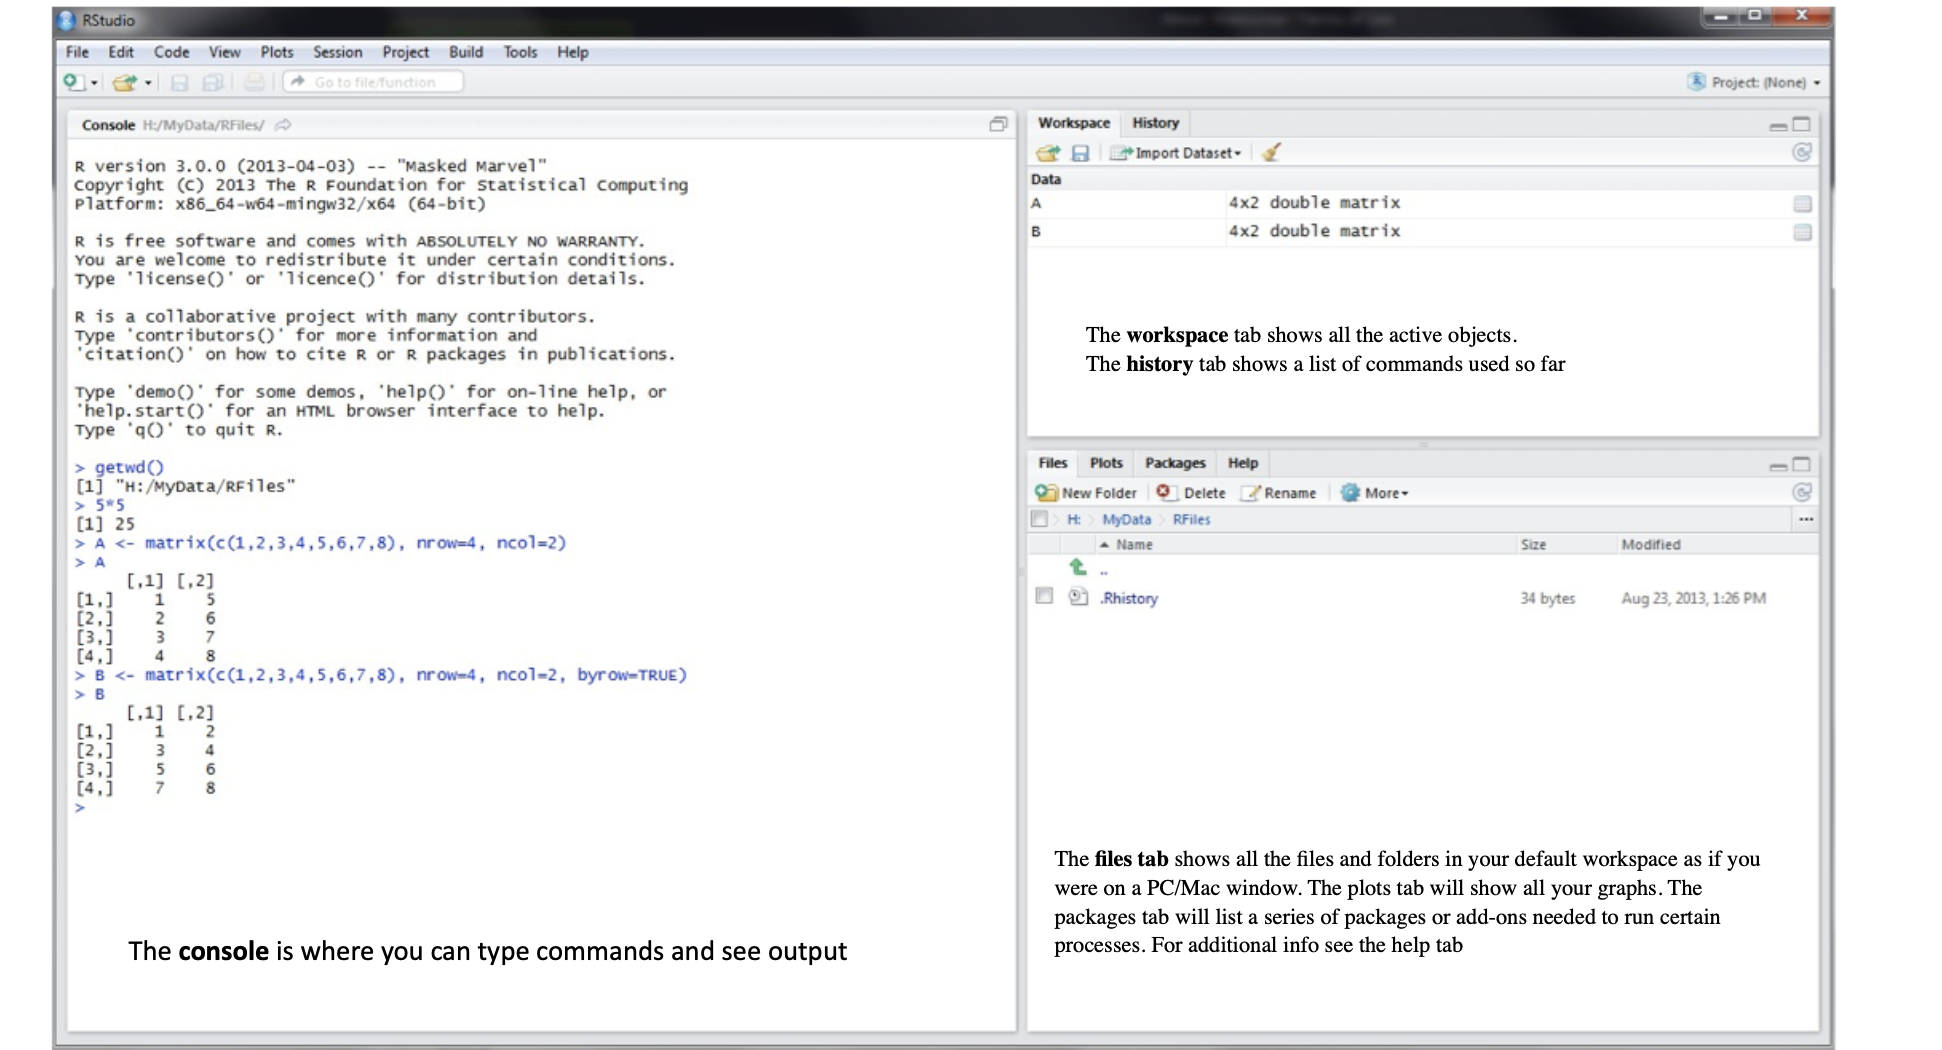
\includegraphics{RStudio.png}
\end{center}

\subsection{Console}\label{console}

Let's focus on the \textbf{console} window on the left. This is where we
can directly communicate with R by entering ``code''. The way this code
is written follows certain arbitrary conventions -- just like natural
languages such as English or German. Here is an example in the R
programming language:

\begin{Shaded}
\begin{Highlighting}[]
\FunctionTok{print}\NormalTok{(}\StringTok{"Hello world!"}\NormalTok{)}
\end{Highlighting}
\end{Shaded}

\begin{verbatim}
[1] "Hello world!"
\end{verbatim}

Entering this command into your console and pressing ENTER will display
the sentence ``Hello world!'' in a new line.

As we can see, anything that R should understand as a simple sequence of
letters or words must be enclosed by quotation marks \texttt{"..."}.
Anything inside them will be interpreted as a so-called \textbf{string}.
Their counterpart are \textbf{numbers} or \textbf{integers}, as
illustrated here:

\begin{Shaded}
\begin{Highlighting}[]
\DecValTok{2} \SpecialCharTok{+} \DecValTok{2} \SpecialCharTok{{-}} \DecValTok{1}
\end{Highlighting}
\end{Shaded}

\begin{verbatim}
[1] 3
\end{verbatim}

Naturally, you can use R for more sophisticated computations:

\begin{itemize}
\item
  \(2 + (3 \times 3)\)

\begin{Shaded}
\begin{Highlighting}[]
\DecValTok{2} \SpecialCharTok{+}\NormalTok{ (}\DecValTok{3} \SpecialCharTok{*} \DecValTok{3}\NormalTok{)}
\end{Highlighting}
\end{Shaded}

\begin{verbatim}
[1] 11
\end{verbatim}
\item
  \(\sqrt{9}\)

\begin{Shaded}
\begin{Highlighting}[]
\FunctionTok{sqrt}\NormalTok{(}\DecValTok{9}\NormalTok{)}
\end{Highlighting}
\end{Shaded}

\begin{verbatim}
[1] 3
\end{verbatim}
\item
  \(\frac{16}{2^3}\)

\begin{Shaded}
\begin{Highlighting}[]
\DecValTok{16} \SpecialCharTok{/} \DecValTok{2} \SpecialCharTok{\^{}} \DecValTok{3}
\end{Highlighting}
\end{Shaded}

\begin{verbatim}
[1] 2
\end{verbatim}
\end{itemize}

\subsection{Working environment}\label{working-environment}

While it is certainly useful to print text or numbers to your console,
it may sometimes make more sense to (at least temporally) store them
somewhere, so you can re-use them later when you need them. In fact, R
gives us a way of storing data in virtual, container-like objects:
\textbf{variables}. We can assign strings or numbers to a variable by
using the assignment operator \texttt{\textless{}-}.

When you run the commands below, you will (hopefully) notice two items
popping up in your \textbf{Environment/Workspace} tab in the top right
corner.

\begin{Shaded}
\begin{Highlighting}[]
\NormalTok{greeting }\OtherTok{\textless{}{-}} \StringTok{"Hello world!"}

\NormalTok{quick\_math }\OtherTok{\textless{}{-}} \DecValTok{2} \SpecialCharTok{+} \DecValTok{2} \SpecialCharTok{{-}} \DecValTok{1}
\end{Highlighting}
\end{Shaded}

If we now want to display the content in the console, we can simply
apply the \texttt{print()} function to the variable itself:

\begin{Shaded}
\begin{Highlighting}[]
\FunctionTok{print}\NormalTok{(greeting)}
\end{Highlighting}
\end{Shaded}

\begin{verbatim}
[1] "Hello world!"
\end{verbatim}

\begin{Shaded}
\begin{Highlighting}[]
\FunctionTok{print}\NormalTok{(quick\_math)}
\end{Highlighting}
\end{Shaded}

\begin{verbatim}
[1] 3
\end{verbatim}

We can also embed variables in other statements. For example, let's take
the content of \texttt{quick\_math} and multiply it with 2.

\begin{Shaded}
\begin{Highlighting}[]
\NormalTok{hard\_math }\OtherTok{\textless{}{-}}\NormalTok{ quick\_math }\SpecialCharTok{*} \DecValTok{2}

\FunctionTok{print}\NormalTok{(hard\_math)}
\end{Highlighting}
\end{Shaded}

\begin{verbatim}
[1] 6
\end{verbatim}

\subsection{R Scripts}\label{r-scripts}

Working with the console has a very plain, yet important disadvantage:
Once we close RStudio, the console is wiped clean, erasing everything
we've typed into it during our precious R session.

The remedy for this nuisance are \textbf{scripts}. Essentially, a script
is the programmer's equivalent of a Word document: It allows you to save
all the code you've written to a file, which you can seamlessly continue
working on the next time you open it.

To \textbf{create a new R script} you can either go to:

\begin{itemize}
\item
  ``File'' \(\rightarrow\) ``New'' \(\rightarrow\) ``R Script'' or
  \ldots{}
\item
  click on the icon with the + sign and select ``R Script'' \ldots{}
\item
  or simply press Ctrl+Shift+N (MacOS: Cmd+Shift+N)
\end{itemize}

Don't forget to save your script with Ctrl+S (Cmd+S)! It is good
practice to save your files regularly.

\chapter{Vectors}\label{vectors}

\section{Recommended reading}\label{recommended-reading}

\begin{quote}
Winter (2020): Chapter 1.1--1.9
\end{quote}

\section{Word frequencies I}\label{word-frequencies-i}

You are given the following token counts of English verb lemmas in the
International Corpus of English:

\begin{longtable}[]{@{}ll@{}}
\toprule\noalign{}
Lemma & Frequency \\
\midrule\noalign{}
\endhead
\bottomrule\noalign{}
\endlastfoot
start & 418 \\
enjoy & 139 \\
begin & 337 \\
help & 281 \\
\end{longtable}

It is always a good idea to visualise frequency data in some way. Quite
conveniently, R happens to provide us with an abundance of plotting
functions. To create a two-dimensional plot, we need to generate two
objects in R: one for the individual lemmas and one for the frequency
counts.

Let's combine the lemmas \emph{start, enjoy, begin} and \emph{help}
using R's \texttt{c()} function and store them in an object
\texttt{lemma}. Enter the following line into a new R script and click
on \textbf{Run} (or simply press Ctrl+Enter/Cmd+Enter).

\begin{Shaded}
\begin{Highlighting}[]
\NormalTok{lemma }\OtherTok{\textless{}{-}} \FunctionTok{c}\NormalTok{(}\StringTok{"start"}\NormalTok{, }\StringTok{"enjoy"}\NormalTok{, }\StringTok{"begin"}\NormalTok{, }\StringTok{"help"}\NormalTok{)}
\end{Highlighting}
\end{Shaded}

We can now do the same for the frequency information:

\begin{Shaded}
\begin{Highlighting}[]
\NormalTok{frequency }\OtherTok{\textless{}{-}} \FunctionTok{c}\NormalTok{(}\DecValTok{418}\NormalTok{, }\DecValTok{139}\NormalTok{, }\DecValTok{337}\NormalTok{, }\DecValTok{281}\NormalTok{)}
\end{Highlighting}
\end{Shaded}

\begin{tcolorbox}[enhanced jigsaw, toprule=.15mm, opacitybacktitle=0.6, coltitle=black, arc=.35mm, colback=white, title=\textcolor{quarto-callout-tip-color}{\faLightbulb}\hspace{0.5em}{When do I use quotation marks?}, titlerule=0mm, toptitle=1mm, bottomtitle=1mm, breakable, rightrule=.15mm, opacityback=0, bottomrule=.15mm, leftrule=.75mm, colframe=quarto-callout-tip-color-frame, left=2mm, colbacktitle=quarto-callout-tip-color!10!white]

Letters and numbers represent two distinct data types in R. Anything
that should be understood as a simple sequence of letters or words must
be enclosed by quotation marks \texttt{"..."}. An expression such as
\texttt{start} will then be evaluated as a \textbf{string}.

\textbf{Numbers} (or \textbf{integers}), by contrast, appear without
quotation marks.

\end{tcolorbox}

Our linguistic data is now stored in two \textbf{variables}
\texttt{lemma} and \texttt{frequency}, which you can conceptualise as
virtual container-like objects. You will also notice that they are now
showing in the \textbf{Environment} tab in the top right corner of
RStudio.

The combination of categorical labels and numeric information renders
our data ideally suited for a barplot. R's most basic barplot function
(which is, unsurprisingly, called \texttt{barplot()}) needs at the very
least \ldots{}

\begin{itemize}
\item
  a \texttt{height} argument, i.e., our y-axis values and
\item
  a \texttt{names.arg} argument, i.e., our x-axis labels.
\end{itemize}

\begin{Shaded}
\begin{Highlighting}[]
\FunctionTok{barplot}\NormalTok{(frequency, }\AttributeTok{names.arg =}\NormalTok{ lemma, }\AttributeTok{col =} \StringTok{"skyblue"}\NormalTok{)}
\end{Highlighting}
\end{Shaded}

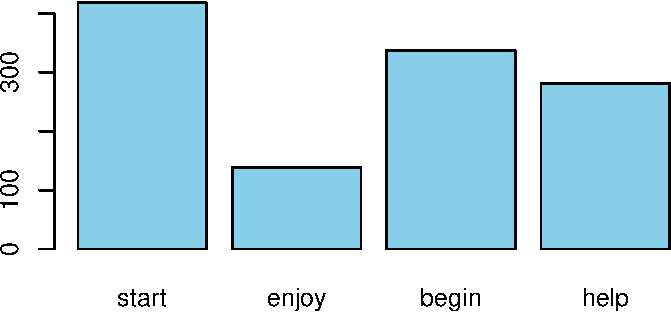
\includegraphics{Vectors_Factors_files/figure-pdf/unnamed-chunk-3-1.pdf}

After some tinkering, our plot looks more presentable:

\begin{Shaded}
\begin{Highlighting}[]
\FunctionTok{barplot}\NormalTok{(frequency, }\AttributeTok{names.arg =}\NormalTok{ lemma, }
        \AttributeTok{main =} \StringTok{"Frequency of Lemmas"}\NormalTok{, }\CommentTok{\# title}
        \AttributeTok{xlab =} \StringTok{"Lemmas"}\NormalTok{,  }\CommentTok{\# label for x{-}axis}
        \AttributeTok{ylab =} \StringTok{"Frequency"}\NormalTok{, }\CommentTok{\# label for y{-}axis}
        \AttributeTok{col =} \StringTok{"steelblue"}\NormalTok{) }\CommentTok{\# color}
\end{Highlighting}
\end{Shaded}

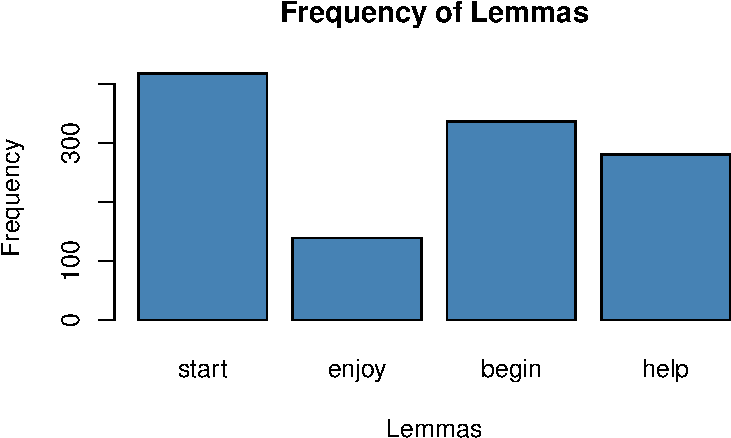
\includegraphics{Vectors_Factors_files/figure-pdf/unnamed-chunk-4-1.pdf}

\begin{tcolorbox}[enhanced jigsaw, toprule=.15mm, opacitybacktitle=0.6, coltitle=black, arc=.35mm, colback=white, title=\textcolor{quarto-callout-tip-color}{\faLightbulb}\hspace{0.5em}{What does `\#' mean? On comments in R}, titlerule=0mm, toptitle=1mm, bottomtitle=1mm, breakable, rightrule=.15mm, opacityback=0, bottomrule=.15mm, leftrule=.75mm, colframe=quarto-callout-tip-color-frame, left=2mm, colbacktitle=quarto-callout-tip-color!10!white]

In R, everything followed by the hashtag \texttt{\#} will be interpreted
as a comment and won't be evaluated by the R compiler. While comments
don't affect the output of our code in the slightest, they are
\textbf{crucial} to any kind of programming project.

Adding prose annotations to your code will make not only it easier to
understand for others but also for your future self. Poor documentation
is a common, yet unnecessary source of frustration for all parties
involved \ldots{}

\begin{center}
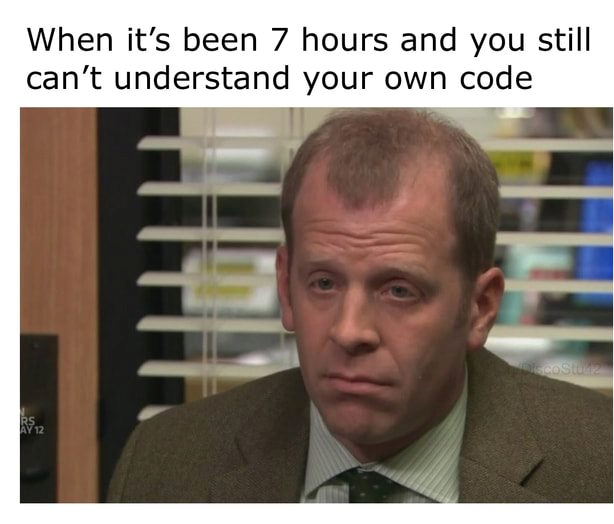
\includegraphics[width=0.6\textwidth,height=\textheight]{comments_meme.png}
\end{center}

\end{tcolorbox}

In RStudio, you now have the option to save the plot to your computer.
Once the figure has appeared in your ``Plots'' panel, you can click on
``Export'' in the menu bar below and proceed to choose the desired
output format and file directory.

\section{Some technical details}\label{some-technical-details}

The example above demonstrates one of the most important data structures
in R: \textbf{Vectors}. They form the cornerstone of various more
complex objects such as data frames, and are essential to handling large
data sets (e.g., corpora). And yet, vectors are very simple in that they
merely constitute one-dimensional sequences of characters or numbers --
no more, no less.

\begin{Shaded}
\begin{Highlighting}[]
\FunctionTok{print}\NormalTok{(lemma)}
\end{Highlighting}
\end{Shaded}

\begin{verbatim}
[1] "start" "enjoy" "begin" "help" 
\end{verbatim}

\begin{Shaded}
\begin{Highlighting}[]
\FunctionTok{print}\NormalTok{(frequency)}
\end{Highlighting}
\end{Shaded}

\begin{verbatim}
[1] 418 139 337 281
\end{verbatim}

The individual elements in these two vectors are not randomly jumbling
around in virtual space, but are in fact following a clear order. Each
element has an ``ID'' (or \textbf{index}), by which we can access it.
For example, if we want to print the first lemma in our \texttt{lemma}
variable, we can use this notation:

\begin{Shaded}
\begin{Highlighting}[]
\NormalTok{lemma[}\DecValTok{1}\NormalTok{]}
\end{Highlighting}
\end{Shaded}

\begin{verbatim}
[1] "start"
\end{verbatim}

Similarly, we can subset \texttt{frequency} according to, for example,
its third element:

\begin{Shaded}
\begin{Highlighting}[]
\NormalTok{frequency[}\DecValTok{3}\NormalTok{]}
\end{Highlighting}
\end{Shaded}

\begin{verbatim}
[1] 337
\end{verbatim}

We can also obtain entire ranges of elements, such as everything from
the second to the fourth one:

\begin{Shaded}
\begin{Highlighting}[]
\NormalTok{frequency[}\DecValTok{2}\SpecialCharTok{:}\DecValTok{4}\NormalTok{]}
\end{Highlighting}
\end{Shaded}

\begin{verbatim}
[1] 139 337 281
\end{verbatim}

\section{Exercises}\label{exercises}

\begin{enumerate}
\def\labelenumi{\arabic{enumi}.}
\tightlist
\item
  Create a vector that lists the third person personal pronouns of
  English (subject and object forms). Store them in a variable
  \texttt{pp3}.
\end{enumerate}

\begin{Shaded}
\begin{Highlighting}[]
\NormalTok{pp3 }\OtherTok{\textless{}{-}} \FunctionTok{c}\NormalTok{(}\StringTok{"he"}\NormalTok{, }\StringTok{"she"}\NormalTok{, }\StringTok{"it"}\NormalTok{, }\StringTok{"him"}\NormalTok{, }\StringTok{"her"}\NormalTok{, }\StringTok{"they"}\NormalTok{, }\StringTok{"them"}\NormalTok{)}
\end{Highlighting}
\end{Shaded}

\begin{enumerate}
\def\labelenumi{\arabic{enumi}.}
\setcounter{enumi}{1}
\item
  Now print \ldots{}

  \begin{itemize}
  \tightlist
  \item
    \ldots{} the fourth element in \texttt{pp3}.
  \end{itemize}

\begin{Shaded}
\begin{Highlighting}[]
\FunctionTok{print}\NormalTok{(pp3[}\DecValTok{4}\NormalTok{]) }\CommentTok{\# or simply}

\NormalTok{pp3[}\DecValTok{4}\NormalTok{]}
\end{Highlighting}
\end{Shaded}

  \begin{itemize}
  \tightlist
  \item
    \ldots{} elements 3 through 5.
  \end{itemize}

\begin{Shaded}
\begin{Highlighting}[]
\NormalTok{pp3[}\DecValTok{3}\SpecialCharTok{:}\DecValTok{5}\NormalTok{]}
\end{Highlighting}
\end{Shaded}

  \begin{itemize}
  \tightlist
  \item
    \ldots{} all elements.
  \end{itemize}

\begin{Shaded}
\begin{Highlighting}[]
\NormalTok{pp3}
\end{Highlighting}
\end{Shaded}

  \begin{itemize}
  \tightlist
  \item
    \ldots{} elements 1, 3 \textbf{and} 5.
  \end{itemize}

\begin{Shaded}
\begin{Highlighting}[]
\NormalTok{pp3[}\FunctionTok{c}\NormalTok{(}\DecValTok{1}\NormalTok{, }\DecValTok{3}\NormalTok{, }\DecValTok{5}\NormalTok{)]}
\end{Highlighting}
\end{Shaded}
\item
  When working with large datasets, we often don't know whether an
  element is in the vector to begin with, let alone its position. For
  instance, if we wanted to check whether \emph{they} is in \texttt{pp3}
  or not, we could use the handy notation below, returning a
  \texttt{TRUE} or \texttt{FALSE} value:
\end{enumerate}

\begin{Shaded}
\begin{Highlighting}[]
\StringTok{"they"} \SpecialCharTok{\%in\%}\NormalTok{ pp3}
\end{Highlighting}
\end{Shaded}

\begin{verbatim}
[1] TRUE
\end{verbatim}

Ascertain whether the following items are in \texttt{pp3}:

\begin{itemize}
\item
  \emph{him}

\begin{Shaded}
\begin{Highlighting}[]
\StringTok{"him"} \SpecialCharTok{\%in\%}\NormalTok{ pp3 }\CommentTok{\# TRUE}
\end{Highlighting}
\end{Shaded}
\item
  \emph{you}

\begin{Shaded}
\begin{Highlighting}[]
\StringTok{"you"} \SpecialCharTok{\%in\%}\NormalTok{ pp3 }\CommentTok{\# FALSE}
\end{Highlighting}
\end{Shaded}
\item
  \emph{it} and \emph{them}

\begin{Shaded}
\begin{Highlighting}[]
\FunctionTok{c}\NormalTok{(}\StringTok{"it"}\NormalTok{, }\StringTok{"them"}\NormalTok{) }\SpecialCharTok{\%in\%}\NormalTok{ pp3 }\CommentTok{\# TRUE TRUE}
\end{Highlighting}
\end{Shaded}
\item
  \emph{we}, \emph{us} and \emph{me}

\begin{Shaded}
\begin{Highlighting}[]
\FunctionTok{c}\NormalTok{(}\StringTok{"we"}\NormalTok{, }\StringTok{"us"}\NormalTok{, }\StringTok{"them"}\NormalTok{) }\SpecialCharTok{\%in\%}\NormalTok{ pp3 }\CommentTok{\# FALSE FALSE TRUE}
\end{Highlighting}
\end{Shaded}
\end{itemize}

\begin{enumerate}
\def\labelenumi{\arabic{enumi}.}
\setcounter{enumi}{3}
\tightlist
\item
  Once we are sure that an element is in the vector of interest, another
  common problem that arises is finding its location. Luckily, R has got
  us covered! The \texttt{which()} function returns the index of an
  element.
\end{enumerate}

\begin{Shaded}
\begin{Highlighting}[]
\FunctionTok{which}\NormalTok{(pp3 }\SpecialCharTok{==} \StringTok{"they"}\NormalTok{) }\CommentTok{\# Note the two equal signs == !}
\end{Highlighting}
\end{Shaded}

\begin{verbatim}
[1] 6
\end{verbatim}

You can read this notation as ``Which element in \texttt{pp3} is
\emph{they}?''. The output suggests that is in position \texttt{6}. Note
that the number obtained depends on the order of elements you've chosen
when creating \texttt{pp3}.

Now, it's your turn: Find the locations of \emph{it} and \emph{them} in
\texttt{pp3}!

\begin{Shaded}
\begin{Highlighting}[]
\CommentTok{\# "him"}
\FunctionTok{which}\NormalTok{(pp3 }\SpecialCharTok{==} \StringTok{"it"}\NormalTok{)}

\CommentTok{\# "you"}
\FunctionTok{which}\NormalTok{(pp3 }\SpecialCharTok{==} \StringTok{"them"}\NormalTok{)}
\end{Highlighting}
\end{Shaded}

\chapter{Data frames}\label{data-frames}

\section{Recommended reading}\label{recommended-reading-1}

\begin{quote}
Winter (2020): Chapter 1.10-1.16
\end{quote}

\section{Word frequencies II}\label{word-frequencies-ii}

Recall our corpus-linguistic data from the previous unit:

\begin{longtable}[]{@{}ll@{}}
\toprule\noalign{}
Lemma & Frequency \\
\midrule\noalign{}
\endhead
\bottomrule\noalign{}
\endlastfoot
start & 418 \\
enjoy & 139 \\
begin & 337 \\
help & 281 \\
\end{longtable}

We thought of the columns as one-dimensional, indexed lists of elements:

\begin{Shaded}
\begin{Highlighting}[]
\NormalTok{lemma }\OtherTok{\textless{}{-}} \FunctionTok{c}\NormalTok{(}\StringTok{"start"}\NormalTok{, }\StringTok{"enjoy"}\NormalTok{, }\StringTok{"begin"}\NormalTok{, }\StringTok{"help"}\NormalTok{)}

\NormalTok{frequency }\OtherTok{\textless{}{-}} \FunctionTok{c}\NormalTok{(}\DecValTok{418}\NormalTok{, }\DecValTok{139}\NormalTok{, }\DecValTok{337}\NormalTok{, }\DecValTok{281}\NormalTok{)}
\end{Highlighting}
\end{Shaded}

Actually, R allows to combine these two vectors into something that
resembles a real spreadsheet. To this end, we need to apply the
\texttt{data.frame()} to two vectors of our choice.

\begin{Shaded}
\begin{Highlighting}[]
\NormalTok{data }\OtherTok{\textless{}{-}} \FunctionTok{data.frame}\NormalTok{(lemma, frequency)}

\FunctionTok{print}\NormalTok{(data)}
\end{Highlighting}
\end{Shaded}

\begin{verbatim}
  lemma frequency
1 start       418
2 enjoy       139
3 begin       337
4  help       281
\end{verbatim}

The variable \texttt{data} is no longer a vector, but a \textbf{data
frame} (often abbreviated as `df'). Once again, each element carries its
own label and can, therefore, be accessed or manipulated.

\section{Some technical details}\label{sec-df}

Since we now have two dimensions, the subsetting notation in square
brackets \texttt{{[}\ {]}} has to reflect that. This is the general
pattern:

\[ df[row, column] \] Following this logic, we can get the element in
the first row of the first column like so:

\begin{Shaded}
\begin{Highlighting}[]
\NormalTok{data[}\DecValTok{1}\NormalTok{,}\DecValTok{1}\NormalTok{]}
\end{Highlighting}
\end{Shaded}

\begin{verbatim}
[1] "start"
\end{verbatim}

If we, however, need the entire first row, we simply omit the column
part. Note that the comma \texttt{,} still needs to be present!

\begin{Shaded}
\begin{Highlighting}[]
\NormalTok{data[}\DecValTok{1}\NormalTok{,]}
\end{Highlighting}
\end{Shaded}

\begin{verbatim}
  lemma frequency
1 start       418
\end{verbatim}

Subsetting by columns is interesting. We can either use the explicit
notation with square brackets or the \textbf{column operator}
\texttt{\$}:

\begin{Shaded}
\begin{Highlighting}[]
\NormalTok{data[,}\DecValTok{1}\NormalTok{]}
\end{Highlighting}
\end{Shaded}

\begin{verbatim}
[1] "start" "enjoy" "begin" "help" 
\end{verbatim}

\begin{Shaded}
\begin{Highlighting}[]
\NormalTok{data}\SpecialCharTok{$}\NormalTok{lemma}
\end{Highlighting}
\end{Shaded}

\begin{verbatim}
[1] "start" "enjoy" "begin" "help" 
\end{verbatim}

\section{Exercises}\label{exercises-1}

\begin{enumerate}
\def\labelenumi{\arabic{enumi}.}
\item
  Recreate the barplot from the previous unit by subsetting the
  \texttt{data} variable accordingly.
\item
\end{enumerate}

\chapter{Libraries}\label{libraries}

\section{Recommended reading}\label{recommended-reading-2}

\begin{quote}
Winter (2020): Chapter 1.13
\end{quote}

\section{Working with packages in R}\label{working-with-packages-in-r}

Packages expand the basic functionality of R by providing numerous
quality-of-life improvements that not only considerably simplify common
data wrangling tasks but which also provide frameworks for
state-of-the-art methods for statistical analysis and natural language
processing (NLP), among many other things.

\subsection{Installation}\label{installation}

\begin{tcolorbox}[enhanced jigsaw, toprule=.15mm, opacitybacktitle=0.6, coltitle=black, arc=.35mm, colback=white, title=\textcolor{quarto-callout-note-color}{\faInfo}\hspace{0.5em}{How do I install a library?}, titlerule=0mm, toptitle=1mm, bottomtitle=1mm, breakable, rightrule=.15mm, opacityback=0, bottomrule=.15mm, leftrule=.75mm, colframe=quarto-callout-note-color-frame, left=2mm, colbacktitle=quarto-callout-note-color!10!white]

Navigate to \texttt{Packages} \textgreater{} \texttt{Install} and verify
that the pop-up window says \texttt{Install\ from:\ Repository\ (CRAN)}.
You can now type in the name of the package you would like to install
under \texttt{Packages}.

\href{https://www.youtube.com/watch?v=u1r5XTqrCTQ}{Video tutorial on
YouTube}

\end{tcolorbox}

This reader will use functions from a variety of R packages. Please
install the following ones:

\begin{itemize}
\item
  \texttt{quanteda} (for the analysis of text data)
\item
  \texttt{tidyverse} (a framework for data manipulation and
  visualisation)
\item
  \texttt{readxl} (for importing Microsoft Excel files)
\item
  \texttt{writexl} (for exporting Microsoft Excel files)
\item
  \texttt{kableExtra} (for creating beautiful tables)
\end{itemize}

\subsection{Loading packages}\label{loading-packages}

Once the installation has been completed, you can proceed to load the
libraries using the code below. You can ignore the warning messages.

\begin{Shaded}
\begin{Highlighting}[]
\FunctionTok{library}\NormalTok{(quanteda)}
\FunctionTok{library}\NormalTok{(tidyverse)}
\FunctionTok{library}\NormalTok{(readxl)}
\FunctionTok{library}\NormalTok{(writexl)}
\FunctionTok{library}\NormalTok{(kableExtra)}
\end{Highlighting}
\end{Shaded}

\begin{tcolorbox}[enhanced jigsaw, toprule=.15mm, opacitybacktitle=0.6, coltitle=black, arc=.35mm, colback=white, title=\textcolor{quarto-callout-note-color}{\faInfo}\hspace{0.5em}{Activating libraries}, titlerule=0mm, toptitle=1mm, bottomtitle=1mm, breakable, rightrule=.15mm, opacityback=0, bottomrule=.15mm, leftrule=.75mm, colframe=quarto-callout-note-color-frame, left=2mm, colbacktitle=quarto-callout-note-color!10!white]

Whenever you start a new R session (i.e., open RStudio), your libraries
and their respective functions will be inactive. To re-activate a
library, either use the \texttt{library()} function or simply select it
in the \texttt{Packages} tab.

\end{tcolorbox}

It is good practice to only activate those packages that are necessary
for your analysis. While it won't be a problem for the small set of
packages as shown here, loading dozens of packages increases the risk of
obtaining ``homonymous'' functions which have the same name but perform
different operations. In this case, it might be helpful to
``disambiguate'' them by directly indicating which package a function is
from:

\begin{Shaded}
\begin{Highlighting}[]
\NormalTok{readxl}\SpecialCharTok{::}\FunctionTok{read\_xlsx}\NormalTok{(...)}
\end{Highlighting}
\end{Shaded}

\chapter{Import/export data}\label{importexport-data}

\section{Recommended reading}\label{recommended-reading-3}

\begin{quote}
Winter (2020): Chapter 1.11
\end{quote}

\section{Preparation}\label{preparation}

The first section of an R-script always specifies the libraries that are
needed for executing the code to follow. In this unit, we will need
\texttt{readxl} and \texttt{writexl} to aid us with importing MS Excel
files.

\begin{Shaded}
\begin{Highlighting}[]
\FunctionTok{library}\NormalTok{(readxl)}
\FunctionTok{library}\NormalTok{(writexl)}
\end{Highlighting}
\end{Shaded}

Simply copy the code lines above into your script and execute them.

\subsection{Exporting data}\label{exporting-data}

Assume we'd like to save our data frame with word frequencies to a local
folder on our system. Let's briefly regenerate it:

\begin{Shaded}
\begin{Highlighting}[]
\NormalTok{lemma }\OtherTok{\textless{}{-}} \FunctionTok{c}\NormalTok{(}\StringTok{"start"}\NormalTok{, }\StringTok{"enjoy"}\NormalTok{, }\StringTok{"begin"}\NormalTok{, }\StringTok{"help"}\NormalTok{)}

\NormalTok{frequency }\OtherTok{\textless{}{-}} \FunctionTok{c}\NormalTok{(}\DecValTok{418}\NormalTok{, }\DecValTok{139}\NormalTok{, }\DecValTok{337}\NormalTok{, }\DecValTok{281}\NormalTok{)}

\NormalTok{data }\OtherTok{\textless{}{-}} \FunctionTok{data.frame}\NormalTok{(lemma, frequency)}

\FunctionTok{print}\NormalTok{(data)}
\end{Highlighting}
\end{Shaded}

\begin{verbatim}
  lemma frequency
1 start       418
2 enjoy       139
3 begin       337
4  help       281
\end{verbatim}

There are two common formats in which tabular data can be stored on your
computer:

\begin{itemize}
\item
  in .\textbf{csv}-files (`\textbf{c}omma-\textbf{s}eparated
  \textbf{v}alues'; native format of LibreOffice)
\item
  .\textbf{xls}/.\textbf{xlsx-files} (Microsoft Excel files)
\end{itemize}

\begin{tcolorbox}[enhanced jigsaw, toprule=.15mm, opacitybacktitle=0.6, coltitle=black, arc=.35mm, colback=white, title=\textcolor{quarto-callout-note-color}{\faInfo}\hspace{0.5em}{Export to CSV}, titlerule=0mm, toptitle=1mm, bottomtitle=1mm, breakable, rightrule=.15mm, opacityback=0, bottomrule=.15mm, leftrule=.75mm, colframe=quarto-callout-note-color-frame, left=2mm, colbacktitle=quarto-callout-note-color!10!white]

To save our \texttt{data} data frame in .csv-format, we can use the
\texttt{write\_table()} function:

\begin{Shaded}
\begin{Highlighting}[]
\FunctionTok{write.csv}\NormalTok{(data, }\StringTok{"frequency\_data.csv"}\NormalTok{)}
\end{Highlighting}
\end{Shaded}

The file is now stored at the location of your current R-script. You can
open this file \ldots{}

\begin{itemize}
\item
  in \textbf{LibreOffice}
\item
  in \textbf{Microsoft Excel} via \texttt{File} \textgreater{}
  \texttt{Import} \textgreater{} \texttt{CSV\ file} \textgreater{}
  Select the file \textgreater{} \texttt{Delimited} and then
  \texttt{Next} \textgreater{} \texttt{Comma} and \texttt{Next}
  \textgreater{} \texttt{General} and \texttt{Finish}.
\end{itemize}

Clearly, opening CSV files in MS Excel is quite cumbersome, which is why
it's better to export it as an Excel file directly.

\end{tcolorbox}

\begin{tcolorbox}[enhanced jigsaw, toprule=.15mm, opacitybacktitle=0.6, coltitle=black, arc=.35mm, colback=white, title=\textcolor{quarto-callout-note-color}{\faInfo}\hspace{0.5em}{Export to Excel}, titlerule=0mm, toptitle=1mm, bottomtitle=1mm, breakable, rightrule=.15mm, opacityback=0, bottomrule=.15mm, leftrule=.75mm, colframe=quarto-callout-note-color-frame, left=2mm, colbacktitle=quarto-callout-note-color!10!white]

We use \texttt{write\_xlsx()} provided by the package \texttt{writexl}
package:

\begin{Shaded}
\begin{Highlighting}[]
\FunctionTok{write\_xlsx}\NormalTok{(data, }\StringTok{"frequency\_data.xlsx"}\NormalTok{)}
\end{Highlighting}
\end{Shaded}

The file is now stored at the location of your current R-script. You
should be able to open it in MS Excel without any issues.

\end{tcolorbox}

\subsection{Importing data}\label{importing-data}

Let's read the two files back into R.

\begin{tcolorbox}[enhanced jigsaw, toprule=.15mm, opacitybacktitle=0.6, coltitle=black, arc=.35mm, colback=white, title=\textcolor{quarto-callout-note-color}{\faInfo}\hspace{0.5em}{Import from CSV}, titlerule=0mm, toptitle=1mm, bottomtitle=1mm, breakable, rightrule=.15mm, opacityback=0, bottomrule=.15mm, leftrule=.75mm, colframe=quarto-callout-note-color-frame, left=2mm, colbacktitle=quarto-callout-note-color!10!white]

To import the CSV file, we can use the \texttt{read.csv()} function:

\begin{Shaded}
\begin{Highlighting}[]
\NormalTok{imported\_csv }\OtherTok{\textless{}{-}} \FunctionTok{read.csv}\NormalTok{(}\StringTok{"frequency\_data.csv"}\NormalTok{)}
\FunctionTok{print}\NormalTok{(imported\_csv)}
\end{Highlighting}
\end{Shaded}

\begin{verbatim}
  X lemma frequency
1 1 start       418
2 2 enjoy       139
3 3 begin       337
4 4  help       281
\end{verbatim}

To get rid of the column with the row names, we'll use some subsetting:

\begin{Shaded}
\begin{Highlighting}[]
\NormalTok{imported\_csv }\OtherTok{\textless{}{-}}\NormalTok{ imported\_csv[,}\SpecialCharTok{{-}}\DecValTok{1}\NormalTok{] }\CommentTok{\# delete first column}
\end{Highlighting}
\end{Shaded}

\end{tcolorbox}

\begin{tcolorbox}[enhanced jigsaw, toprule=.15mm, opacitybacktitle=0.6, coltitle=black, arc=.35mm, colback=white, title=\textcolor{quarto-callout-note-color}{\faInfo}\hspace{0.5em}{Import from Excel}, titlerule=0mm, toptitle=1mm, bottomtitle=1mm, breakable, rightrule=.15mm, opacityback=0, bottomrule=.15mm, leftrule=.75mm, colframe=quarto-callout-note-color-frame, left=2mm, colbacktitle=quarto-callout-note-color!10!white]

For importing the Excel file, we'll use the \texttt{read\_xlsx()}
function from the readxl package:

\begin{Shaded}
\begin{Highlighting}[]
\NormalTok{imported\_excel }\OtherTok{\textless{}{-}} \FunctionTok{read\_xlsx}\NormalTok{(}\StringTok{"frequency\_data.xlsx"}\NormalTok{)}
\FunctionTok{print}\NormalTok{(imported\_excel)}
\end{Highlighting}
\end{Shaded}

\begin{verbatim}
# A tibble: 4 x 2
  lemma frequency
  <chr>     <dbl>
1 start       418
2 enjoy       139
3 begin       337
4 help        281
\end{verbatim}

\end{tcolorbox}

That's it! Nevertheless, remember to always check your imported data to
ensure it has been read correctly, especially when working with CSV
files.

\subsection{Exercises}\label{exercises-2}

\part{Corpus linguistics with R}

\chapter{Concordancing}\label{concordancing}

\section{\texorpdfstring{Using the
\texttt{QuantedaApp}}{Using the QuantedaApp}}\label{using-the-quantedaapp}

Installation and usage instructions are available in this
\href{https://github.com/VBuskin/quanteda_app}{GitHub repository}.

\section{\texorpdfstring{Using the \texttt{quanteda} package in
R}{Using the quanteda package in R}}\label{using-the-quanteda-package-in-r}

\subsection{Preparation}\label{preparation-1}

\begin{tcolorbox}[enhanced jigsaw, toprule=.15mm, opacitybacktitle=0.6, coltitle=black, arc=.35mm, colback=white, title=\textcolor{quarto-callout-warning-color}{\faExclamationTriangle}\hspace{0.5em}{Working directory}, titlerule=0mm, toptitle=1mm, bottomtitle=1mm, breakable, rightrule=.15mm, opacityback=0, bottomrule=.15mm, leftrule=.75mm, colframe=quarto-callout-warning-color-frame, left=2mm, colbacktitle=quarto-callout-warning-color!10!white]

In order for R to be able to recognise the data, it is crucial to set up
the working directory correctly.

\begin{enumerate}
\def\labelenumi{\arabic{enumi}.}
\item
  Make sure your R-script \textbf{and} the corpus (e.g., `ICE-GB') are
  stored in the \textbf{same folder}.
\item
  In RStudio, now navigate to \texttt{Session} \textgreater{}
  \texttt{Set\ working\ directory} \textgreater{}
  \texttt{To\ Source\ File\ Location}. This ensures that the folder
  where you have placed your R-script will function as your working
  directory until you close RStudio again.
\end{enumerate}

To see your working directory in your files pane, click on
\texttt{Files} \textgreater{}
\texttt{\textquotesingle{}Blue\ wheel\ symbol\textquotesingle{}}
\textgreater{} \texttt{Go\ to\ working\ directory}.

\end{tcolorbox}

\subsection{Loading the corpus}\label{loading-the-corpus}

To load a corpus object into R, place it in your working directory and
perform read it into your working environment with \texttt{readRDS()}.
The ICE-GB.RDS file you've been provided with has been pre-processed and
saved in this specific format for practical reasons.

\begin{Shaded}
\begin{Highlighting}[]
\NormalTok{ICE\_GB }\OtherTok{\textless{}{-}} \FunctionTok{readRDS}\NormalTok{(}\StringTok{"ICE\_GB.RDS"}\NormalTok{)}
\end{Highlighting}
\end{Shaded}

If you encounter any error messages, make sure you followed steps 1 and
2 in the box above.

\subsection{Concordancing}\label{concordancing-1}

In order to perform concordances in R, we need to load the packages
below.

\begin{Shaded}
\begin{Highlighting}[]
\CommentTok{\# Load libraries}
\FunctionTok{library}\NormalTok{(quanteda)}
\FunctionTok{library}\NormalTok{(tidyverse)}
\end{Highlighting}
\end{Shaded}

Next, we use the \texttt{kwic()} function, which requires a corpus
object and a search expression. Let's supply both:

\begin{Shaded}
\begin{Highlighting}[]
\CommentTok{\# Query the corpus}
\NormalTok{query1 }\OtherTok{\textless{}{-}} \FunctionTok{kwic}\NormalTok{(ICE\_GB, }\FunctionTok{phrase}\NormalTok{(}\StringTok{"eat"}\NormalTok{))}
\end{Highlighting}
\end{Shaded}

Print the first few lines of our results with \texttt{head()}:

\begin{Shaded}
\begin{Highlighting}[]
\FunctionTok{head}\NormalTok{(query1)}
\end{Highlighting}
\end{Shaded}

\begin{verbatim}
Keyword-in-context with 6 matches.                                                            
  [ICE_GB/S1A-006.txt, 785]           So I' d rather | eat |
 [ICE_GB/S1A-009.txt, 1198]              I must <, > | eat |
  [ICE_GB/S1A-010.txt, 958]         to <, > actually | eat |
  [ICE_GB/S1A-018.txt, 455] order one first and then | eat |
  [ICE_GB/S1A-018.txt, 498]  A > The bargain hunting | eat |
 [ICE_GB/S1A-023.txt, 1853]       B > Oh name please | eat |
                            
 beforehand just to avoid uh
 them < ICE-GB:S1A-009#71:  
 it for one' s              
 it and then sort of        
 < ICE-GB:S1A-018#29: 1     
 something <,, >            
\end{verbatim}

\begin{table}
\centering
\begin{tabular}[t]{l|r|r|l|l|l|l}
\hline
docname & from & to & pre & keyword & post & pattern\\
\hline
ICE\_GB/S1A-006.txt & 785 & 785 & So I ' d rather & eat & beforehand just to avoid uh & eat\\
\hline
ICE\_GB/S1A-009.txt & 1198 & 1198 & I must < , > & eat & them < ICE-GB:S1A-009 \#71 : & eat\\
\hline
ICE\_GB/S1A-010.txt & 958 & 958 & to < , > actually & eat & it for one ' s & eat\\
\hline
ICE\_GB/S1A-018.txt & 455 & 455 & order one first and then & eat & it and then sort of & eat\\
\hline
ICE\_GB/S1A-018.txt & 498 & 498 & A > The bargain hunting & eat & < ICE-GB:S1A-018 \#29 : 1 & eat\\
\hline
ICE\_GB/S1A-023.txt & 1853 & 1853 & B > Oh name please & eat & something < , , > & eat\\
\hline
\end{tabular}
\end{table}

For a full screen display of the data frame, try \texttt{View()}:

\begin{Shaded}
\begin{Highlighting}[]
\FunctionTok{View}\NormalTok{(query1)}
\end{Highlighting}
\end{Shaded}

\subsection{Some basic statistics}\label{some-basic-statistics}

How many tokens (= individual hits) does our query return?

\begin{Shaded}
\begin{Highlighting}[]
\FunctionTok{nrow}\NormalTok{(query1) }\CommentTok{\# Token number corresponds to the number of rows in the data frame}
\end{Highlighting}
\end{Shaded}

\begin{verbatim}
[1] 53
\end{verbatim}

How many types (= distinct hits) does our query return?

\begin{Shaded}
\begin{Highlighting}[]
\FunctionTok{table}\NormalTok{(query1}\SpecialCharTok{$}\NormalTok{keyword)}
\end{Highlighting}
\end{Shaded}

\begin{verbatim}

eat Eat 
 52   1 
\end{verbatim}

How is the keyword distributed across corpus files?

\begin{Shaded}
\begin{Highlighting}[]
\NormalTok{query\_distrib }\OtherTok{\textless{}{-}} \FunctionTok{table}\NormalTok{(query1}\SpecialCharTok{$}\NormalTok{docname, query1}\SpecialCharTok{$}\NormalTok{keyword)}

\FunctionTok{head}\NormalTok{(query\_distrib, }\AttributeTok{n =} \DecValTok{10}\NormalTok{)}
\end{Highlighting}
\end{Shaded}

\begin{verbatim}
                    
                     eat Eat
  ICE_GB/S1A-006.txt   1   0
  ICE_GB/S1A-009.txt   1   0
  ICE_GB/S1A-010.txt   1   0
  ICE_GB/S1A-018.txt   2   0
  ICE_GB/S1A-023.txt   1   0
  ICE_GB/S1A-025.txt   1   0
  ICE_GB/S1A-038.txt   1   0
  ICE_GB/S1A-046.txt   2   0
  ICE_GB/S1A-047.txt   3   0
  ICE_GB/S1A-051.txt   1   0
\end{verbatim}

\subsection{Window size}\label{window-size}

Some studies require careful examination of the preceding or following
context of the keyword. We can easily adjust the \texttt{window} size to
suit our needs:

\begin{Shaded}
\begin{Highlighting}[]
\NormalTok{query2 }\OtherTok{\textless{}{-}} \FunctionTok{kwic}\NormalTok{(ICE\_GB, }\FunctionTok{phrase}\NormalTok{(}\StringTok{"eat"}\NormalTok{), }\AttributeTok{window =} \DecValTok{20}\NormalTok{) }
\end{Highlighting}
\end{Shaded}

\begin{table}
\centering
\begin{tabular}[t]{l|r|r|l|l|l|l}
\hline
docname & from & to & pre & keyword & post & pattern\\
\hline
ICE\_GB/S1A-006.txt & 785 & 785 & \#49 : 1 : A > Yeah < ICE-GB:S1A-006 \#50 : 1 : A > So I ' d rather & eat & beforehand just to avoid uh < , , > any problems there < ICE-GB:S1A-006 \#51 : 1 : B > & eat\\
\hline
ICE\_GB/S1A-009.txt & 1198 & 1198 & < , > in in the summer < ICE-GB:S1A-009 \#70 : 1 : A > I must < , > & eat & them < ICE-GB:S1A-009 \#71 : 1 : A > Yes < ICE-GB:S1A-009 \#72 : 1 : B > You ought & eat\\
\hline
ICE\_GB/S1A-010.txt & 958 & 958 & 1 : B > You know I mean it would seem to be squandering it to < , > actually & eat & it for one ' s own enjoyment < , , > < ICE-GB:S1A-010 \#49 : 1 : A > Mm & eat\\
\hline
ICE\_GB/S1A-018.txt & 455 & 455 & s so < ICE-GB:S1A-018 \#27 : 1 : A > What you should do is order one first and then & eat & it and then sort of carry on from there < laughter > < , > by which time you wouldn't & eat\\
\hline
ICE\_GB/S1A-018.txt & 498 & 498 & second anyway so < laugh > < , > < ICE-GB:S1A-018 \#28 : 1 : A > The bargain hunting & eat & < ICE-GB:S1A-018 \#29 : 1 : B > So all right what did I have < ICE-GB:S1A-018 \#30 : 1 & eat\\
\hline
ICE\_GB/S1A-023.txt & 1853 & 1853 & > I can't bear it < , , > < ICE-GB:S1A-023 \#121 : 1 : B > Oh name please & eat & something < , , > < ICE-GB:S1A-023 \#122 : 1 : A > Oh actually Dad asked me if < & eat\\
\hline
\end{tabular}
\end{table}

\subsection{Saving your output}\label{saving-your-output}

You can store your results in a spreadsheet file just as described in
\texttt{Introduction\ to\ R\ \textgreater{}\ Import/export\ data}.

\begin{itemize}
\tightlist
\item
  \textbf{Microsoft Excel (.xlsx)}
\end{itemize}

\begin{Shaded}
\begin{Highlighting}[]
\FunctionTok{library}\NormalTok{(writexl)}

\FunctionTok{write\_xlsx}\NormalTok{(query2, }\StringTok{"myresults1.xlsx"}\NormalTok{)}
\end{Highlighting}
\end{Shaded}

\begin{itemize}
\tightlist
\item
  \textbf{LibreOffice} (.csv)
\end{itemize}

\begin{Shaded}
\begin{Highlighting}[]
\FunctionTok{write.csv}\NormalTok{(query2, }\StringTok{"myresults1.csv"}\NormalTok{)}
\end{Highlighting}
\end{Shaded}

As soon as you have annotated your data, you can load .xlsx files back
into R with \texttt{read\_xlsx()} from the \texttt{readxl} package and
.csv files using the Base R function \texttt{read.csv()}.

\chapter{Regular expressions}\label{regular-expressions}

\section{Regular expressions}\label{regular-expressions-1}

\textbf{Regular expressions} (or `regex') help us find more complex
patterns in strings of text. Suppose we are interested in finding all
inflectional forms of the lemma PROVIDE in a corpus, i.e.,
\emph{provide, provides, providing} and \emph{provided}. Insteading of
searching for all forms individually, we can construct a regular
expression of the form

\[
\text{provid(es | ing | ed)?}
\]which can be read as `Match the sequence of letters
\textless provide\textgreater{} as well as when it is optionally
followed by the letters \textless s\textgreater{} or
\textless ing\textgreater{} or \textless ed\textgreater{}'. Notice how
optionality is signified by the `?' operator and alternatives by
`\textbar{}'.

To activate regular expression in a KWIC query, simply set the
\texttt{valuetype} argument to \texttt{"regex"}:

\begin{Shaded}
\begin{Highlighting}[]
\CommentTok{\# Load library and corpus}
\FunctionTok{library}\NormalTok{(quanteda)}
\NormalTok{ICE\_GB }\OtherTok{\textless{}{-}} \FunctionTok{readRDS}\NormalTok{(}\StringTok{"ICE\_GB.RDS"}\NormalTok{)}

\CommentTok{\# Perform query}
\NormalTok{kwic\_provide }\OtherTok{\textless{}{-}} \FunctionTok{kwic}\NormalTok{(ICE\_GB,}
                     \FunctionTok{phrase}\NormalTok{(}\StringTok{"provid(es|ing|ed)?"}\NormalTok{),}
                     \AttributeTok{valuetype =} \StringTok{"regex"}\NormalTok{,}
                     \AttributeTok{window =} \DecValTok{20}\NormalTok{)}
\end{Highlighting}
\end{Shaded}

The number of hits has more than doubled. However, upon closer
inspection, we'll notice a few false positives, namely
\emph{providential, provider} and \emph{providers}:

\begin{Shaded}
\begin{Highlighting}[]
\FunctionTok{table}\NormalTok{(kwic\_provide}\SpecialCharTok{$}\NormalTok{keyword)}
\end{Highlighting}
\end{Shaded}

\begin{verbatim}

      provid      provide     provided     Provided    Provident providential 
           1          165          118            5            1            1 
    provider    providers     provides    providing    Providing 
           1            3           72           52            1 
\end{verbatim}

There are two ways to handle this:

\begin{enumerate}
\def\labelenumi{\arabic{enumi}.}
\tightlist
\item
  Refine the search expression further to only match those cases of
  interest.
\item
  Manually sort out irrelevant cases during annotation in your
  spreadsheet software.
\end{enumerate}

As a rule of thumb, you should consider improving your search expression
if you receive hundreds or even thousands of false hits. If there are
only a couple of false positives, it's usually easier to simply mark
them as ``irrelevant'' in your spreadsheet.

\begin{tcolorbox}[enhanced jigsaw, toprule=.15mm, opacitybacktitle=0.6, coltitle=black, arc=.35mm, colback=white, title=\textcolor{quarto-callout-caution-color}{\faFire}\hspace{0.5em}{Task}, titlerule=0mm, toptitle=1mm, bottomtitle=1mm, breakable, rightrule=.15mm, opacityback=0, bottomrule=.15mm, leftrule=.75mm, colframe=quarto-callout-caution-color-frame, left=2mm, colbacktitle=quarto-callout-caution-color!10!white]

How could you refine the search expression for PROVIDE to get rid of the
irrelevant cases? Consult the RegEX Cheatsheet below!

\begin{Shaded}
\begin{Highlighting}[]
\CommentTok{\# Add word boundary with \textbackslash{}\textbackslash{}b}
\NormalTok{kwic\_provide2 }\OtherTok{\textless{}{-}} \FunctionTok{kwic}\NormalTok{(ICE\_GB,}
                     \FunctionTok{phrase}\NormalTok{(}\StringTok{"}\SpecialCharTok{\textbackslash{}\textbackslash{}}\StringTok{bprovid(e|es|ing|ed)}\SpecialCharTok{\textbackslash{}\textbackslash{}}\StringTok{b"}\NormalTok{),}
                     \AttributeTok{valuetype =} \StringTok{"regex"}\NormalTok{,}
                     \AttributeTok{window =} \DecValTok{20}\NormalTok{)}

\FunctionTok{table}\NormalTok{(kwic\_provide2}\SpecialCharTok{$}\NormalTok{keyword)}
\end{Highlighting}
\end{Shaded}

\end{tcolorbox}

\section{A RegEx Cheatsheet}\label{a-regex-cheatsheet}

\subsection{Basic functions}\label{basic-functions}

\begin{longtable}[]{@{}llll@{}}
\toprule\noalign{}
\textbf{Command} & \textbf{Definition} & \textbf{Example} &
\textbf{Finds} \\
\midrule\noalign{}
\endhead
\bottomrule\noalign{}
\endlastfoot
& & \texttt{python} & \emph{python} \\
\texttt{.} & Any character & \texttt{.ython} & \emph{aython,
bython\ldots{}} \\
\end{longtable}

\subsection{Character classes and
alternatives}\label{character-classes-and-alternatives}

\begin{longtable}[]{@{}
  >{\raggedright\arraybackslash}p{(\columnwidth - 6\tabcolsep) * \real{0.2297}}
  >{\raggedright\arraybackslash}p{(\columnwidth - 6\tabcolsep) * \real{0.3108}}
  >{\raggedright\arraybackslash}p{(\columnwidth - 6\tabcolsep) * \real{0.2297}}
  >{\raggedright\arraybackslash}p{(\columnwidth - 6\tabcolsep) * \real{0.2297}}@{}}
\toprule\noalign{}
\begin{minipage}[b]{\linewidth}\raggedright
\textbf{Command}
\end{minipage} & \begin{minipage}[b]{\linewidth}\raggedright
\textbf{Definition}
\end{minipage} & \begin{minipage}[b]{\linewidth}\raggedright
\textbf{Example}
\end{minipage} & \begin{minipage}[b]{\linewidth}\raggedright
\textbf{Finds}
\end{minipage} \\
\midrule\noalign{}
\endhead
\bottomrule\noalign{}
\endlastfoot
\texttt{{[}abc{]}} & Class of characters & \texttt{{[}jp{]}ython} &
\emph{jython, python} \\
\texttt{{[}\ \^{}pP{]}} & Excluded class of characters &
\texttt{{[}\^{}pP{]}ython} & everything but \emph{python, Python} \\
\texttt{(...\textbar{}...)} & Alternatives linked by logical operator
\texttt{or} & \texttt{P(ython\textbar{}eter)} & \emph{Python, Peter} \\
\end{longtable}

\subsection{Pre-defined character
classes}\label{pre-defined-character-classes}

\begin{longtable}[]{@{}
  >{\raggedright\arraybackslash}p{(\columnwidth - 6\tabcolsep) * \real{0.2361}}
  >{\raggedright\arraybackslash}p{(\columnwidth - 6\tabcolsep) * \real{0.2917}}
  >{\raggedright\arraybackslash}p{(\columnwidth - 6\tabcolsep) * \real{0.2361}}
  >{\raggedright\arraybackslash}p{(\columnwidth - 6\tabcolsep) * \real{0.2361}}@{}}
\toprule\noalign{}
\begin{minipage}[b]{\linewidth}\raggedright
\textbf{Command}
\end{minipage} & \begin{minipage}[b]{\linewidth}\raggedright
\textbf{Definition}
\end{minipage} & \begin{minipage}[b]{\linewidth}\raggedright
\textbf{Example}
\end{minipage} & \begin{minipage}[b]{\linewidth}\raggedright
\textbf{Finds}
\end{minipage} \\
\midrule\noalign{}
\endhead
\bottomrule\noalign{}
\endlastfoot
\texttt{\textbackslash{}\textbackslash{}w} & All alphanumeric characters
& & A-Z, a-z, 0-9 \\
\texttt{\textbackslash{}\textbackslash{}W} & All non-alphanumeric
characters & & everything but A-Z, a-z, 0-9 \\
\texttt{\textbackslash{}\textbackslash{}d} & All decimal numbers & &
0-9 \\
\texttt{\textbackslash{}\textbackslash{}D} & Everything which is not a
decimal number & & everything but 0-9 \\
\texttt{\textbackslash{}\textbackslash{}s} & Empty space & & \\
\texttt{\textbackslash{}\textbackslash{}b} & Word boundary &
\texttt{\textbackslash{}\textbackslash{}bpython\textbackslash{}\textbackslash{}b}
& Matches \emph{python} as a whole word \\
\end{longtable}

\subsection{Quantifiers}\label{quantifiers}

\begin{longtable}[]{@{}
  >{\raggedright\arraybackslash}p{(\columnwidth - 6\tabcolsep) * \real{0.2297}}
  >{\raggedright\arraybackslash}p{(\columnwidth - 6\tabcolsep) * \real{0.3108}}
  >{\raggedright\arraybackslash}p{(\columnwidth - 6\tabcolsep) * \real{0.2297}}
  >{\raggedright\arraybackslash}p{(\columnwidth - 6\tabcolsep) * \real{0.2297}}@{}}
\toprule\noalign{}
\begin{minipage}[b]{\linewidth}\raggedright
\textbf{Command}
\end{minipage} & \begin{minipage}[b]{\linewidth}\raggedright
\textbf{Definition}
\end{minipage} & \begin{minipage}[b]{\linewidth}\raggedright
\textbf{Example}
\end{minipage} & \begin{minipage}[b]{\linewidth}\raggedright
\textbf{Finds}
\end{minipage} \\
\midrule\noalign{}
\endhead
\bottomrule\noalign{}
\endlastfoot
\texttt{?} & One or zero instances of the preceding symbol &
\texttt{Py?thon} & \emph{Python, Pthon} \\
\texttt{*} & No matter how many times --- also zero & \texttt{Py*thon} &
\emph{Python, Pthon, Pyyyython\ldots{}} \\
& & \texttt{P{[}Yy{]}*thon} & \emph{Python, Pthon, PyYYython\ldots{}} \\
\texttt{+} & No matter how many times but at least once &
\texttt{Py+thon} & \emph{Python, Pyyython, Pyyyython} \\
\texttt{\{1,3\}} & \texttt{\{min,\ max\}} & \texttt{Py\{1,3\}thon} &
\emph{Python, Pyython, Pyyython} \\
\end{longtable}

\section{Exercises}\label{exercises-3}

\begin{enumerate}
\def\labelenumi{\arabic{enumi}.}
\tightlist
\item
  Find all labels of months!
\item
  Write an elegant regular expression which finds \emph{sing},
  \emph{sang} and \emph{sung}.
\item
  Find all four-digit numbers in the corpus!
\item
  Write an elegant regular expression which finds all inflectional forms
  of \emph{swim}!
\end{enumerate}

\part{Descriptive statistics}

\chapter{Statistical variables}\label{statistical-variables}

\section{Preparation}\label{preparation-2}

Please download the file \texttt{Paquot\_Larsson\_2020\_data.xlsx}
(Paquot and Larsson 2020)\footnote{The supplementary materials can be
  downloaded from the publisher's
  \href{https://link.springer.com/chapter/10.1007/978-3-030-46216-1_17}{website}
  {[}Last accessed April 28, 2024{]}. Note that the dataset has been
  originally compiled by Gries (2013).} and store it in your working
directory.

\begin{Shaded}
\begin{Highlighting}[]
\CommentTok{\# Libraries}
\FunctionTok{library}\NormalTok{(}\StringTok{"readxl"}\NormalTok{)}
\FunctionTok{library}\NormalTok{(}\StringTok{"tidyverse"}\NormalTok{)}

\CommentTok{\# Load data}
\NormalTok{cl.order }\OtherTok{\textless{}{-}} \FunctionTok{read\_xlsx}\NormalTok{(}\StringTok{"Paquot\_Larsson\_2020\_data.xlsx"}\NormalTok{)}

\CommentTok{\# Inspect data}
\FunctionTok{str}\NormalTok{(cl.order)}
\end{Highlighting}
\end{Shaded}

\begin{verbatim}
tibble [403 x 8] (S3: tbl_df/tbl/data.frame)
 $ CASE       : num [1:403] 4777 1698 953 1681 4055 ...
 $ ORDER      : chr [1:403] "sc-mc" "mc-sc" "sc-mc" "mc-sc" ...
 $ SUBORDTYPE : chr [1:403] "temp" "temp" "temp" "temp" ...
 $ LEN_MC     : num [1:403] 4 7 12 6 9 9 9 4 6 4 ...
 $ LEN_SC     : num [1:403] 10 6 7 15 5 5 12 2 24 11 ...
 $ LENGTH_DIFF: num [1:403] -6 1 5 -9 4 4 -3 2 -18 -7 ...
 $ CONJ       : chr [1:403] "als/when" "als/when" "als/when" "als/when" ...
 $ MORETHAN2CL: chr [1:403] "no" "no" "yes" "no" ...
\end{verbatim}

\begin{Shaded}
\begin{Highlighting}[]
\FunctionTok{head}\NormalTok{(cl.order)}
\end{Highlighting}
\end{Shaded}

\begin{verbatim}
# A tibble: 6 x 8
   CASE ORDER SUBORDTYPE LEN_MC LEN_SC LENGTH_DIFF CONJ     MORETHAN2CL
  <dbl> <chr> <chr>       <dbl>  <dbl>       <dbl> <chr>    <chr>      
1  4777 sc-mc temp            4     10          -6 als/when no         
2  1698 mc-sc temp            7      6           1 als/when no         
3   953 sc-mc temp           12      7           5 als/when yes        
4  1681 mc-sc temp            6     15          -9 als/when no         
5  4055 sc-mc temp            9      5           4 als/when yes        
6   967 sc-mc temp            9      5           4 als/when yes        
\end{verbatim}

\section{Types of variables}\label{types-of-variables}

The concept of the \textbf{variable} allows us to quantify various
aspects of our observations.

\begin{itemize}
\item
  \textbf{nominal/categorical}: These variables have a limited number of
  levels which cannot be ordered in a meaningful way. For instance, it
  does not matter which value of \texttt{SUBORDTYPE} or
  \texttt{MORETHAN2CL} comes first or last:

\begin{Shaded}
\begin{Highlighting}[]
\FunctionTok{unique}\NormalTok{(cl.order}\SpecialCharTok{$}\NormalTok{SUBORDTYPE)}
\end{Highlighting}
\end{Shaded}

\begin{verbatim}
[1] "temp" "caus"
\end{verbatim}

\begin{Shaded}
\begin{Highlighting}[]
\FunctionTok{unique}\NormalTok{(cl.order}\SpecialCharTok{$}\NormalTok{MORETHAN2CL)}
\end{Highlighting}
\end{Shaded}

\begin{verbatim}
[1] "no"  "yes"
\end{verbatim}
\item
  \textbf{ordinal}: Such variables can be ordered, but the intervals
  between their individuals values are not meaningful. Heumann (2022: 6)
  provides a pertinent example:

  ``{[}T{]}he satisfaction with a product (unsatisfied--satisfied--very
  satisfied) is an ordinal variable because the values this variable can
  take can be ordered but the differences between
  `unsatisfied--satisfied' and `satisfied--very satisfied' cannot be
  compared in a numerical way''.
\item
  In the case of \textbf{interval}-scaled variables, the differences
  between the values can be interpreted, but their ratios must be
  treated with caution. A temperature of 4°C is 6 degrees warmer than
  -2°C; however, this does not imply that 4°C is three times warmer than
  -2°C. This is because the temperature scale has no true zero point;
  0°C simply signifies another point on the scale and not the absence of
  temperature altogether.
\item
  \textbf{Ratio}-scaled variables allow both a meaningful interpretation
  of the differences between their values and (!) of the ratios between
  them. Within the context of clause length, \texttt{LENGTH\_DIFF}
  values such as 4 and 8 not only suggest that the latter is four units
  greater than the former but also that their ratio \(\frac{8}{4} = 2\)
  is a valid way to describe the relationship between these values. Here
  a \texttt{LENGTH\_DIFF} of 0 can be clearly viewed as the absence of a
  length difference.
\end{itemize}

\chapter{Categorical data}\label{categorical-data}

\section{Preparation}\label{preparation-3}

Please download the file ``Paquot\_Larsson\_2020\_data.xlsx'' (Paquot
and Larsson 2020)\footnote{The original supplementary materials can be
  downloaded from the publisher's
  \href{https://link.springer.com/chapter/10.1007/978-3-030-46216-1_17}{website}
  {[}Last accessed April 28, 2024{]}.} and store it in the same folder
as your currently active R-script.

\begin{Shaded}
\begin{Highlighting}[]
\CommentTok{\# Libraries}
\FunctionTok{library}\NormalTok{(}\StringTok{"readxl"}\NormalTok{)}
\FunctionTok{library}\NormalTok{(}\StringTok{"tidyverse"}\NormalTok{)}

\CommentTok{\# Load data from working directory}
\NormalTok{cl.order }\OtherTok{\textless{}{-}} \FunctionTok{read\_xlsx}\NormalTok{(}\StringTok{"Paquot\_Larsson\_2020\_data.xlsx"}\NormalTok{)}
\end{Highlighting}
\end{Shaded}

It contains the \textbf{dependent variable}

\begin{itemize}
\tightlist
\item
  \texttt{ORDER}: Does the subordinate clause come before or after the
  main clause? (`sc-mc' vs.~`mc-sc')
\end{itemize}

\ldots{} and the \textbf{independent variables}:

\begin{itemize}
\item
  \texttt{SUBORDTYPE}: Is the subordinate clause temporal or causal?
  (`temp' vs.~`caus')
\item
  \texttt{MORETHAN2CL}: Are there most clauses in the sentence than just
  one subordinate clause and one main clause? (`yes' vs.~`no')
\item
  \texttt{LEN\_MC}: How many words does the main clause contain?
  (ratio-scaled continuous variable)
\item
  \texttt{LEN\_SC}: How many words does the subordinate clause contain?
  (ratio-scaled continuous variable)
\item
  \texttt{LENGTH\_DIFF}: What is the length difference in words between
  the main clause and subordinate clause? (ratio-scaled continuous
  variables)
\end{itemize}

\section{Descriptive measures}\label{descriptive-measures}

The easiest way to get a general overview of the full data set is to
apply the \texttt{str()} function to the respective data frame.

\begin{Shaded}
\begin{Highlighting}[]
\FunctionTok{str}\NormalTok{(cl.order)}
\end{Highlighting}
\end{Shaded}

\begin{verbatim}
tibble [403 x 8] (S3: tbl_df/tbl/data.frame)
 $ CASE       : num [1:403] 4777 1698 953 1681 4055 ...
 $ ORDER      : chr [1:403] "sc-mc" "mc-sc" "sc-mc" "mc-sc" ...
 $ SUBORDTYPE : chr [1:403] "temp" "temp" "temp" "temp" ...
 $ LEN_MC     : num [1:403] 4 7 12 6 9 9 9 4 6 4 ...
 $ LEN_SC     : num [1:403] 10 6 7 15 5 5 12 2 24 11 ...
 $ LENGTH_DIFF: num [1:403] -6 1 5 -9 4 4 -3 2 -18 -7 ...
 $ CONJ       : chr [1:403] "als/when" "als/when" "als/when" "als/when" ...
 $ MORETHAN2CL: chr [1:403] "no" "no" "yes" "no" ...
\end{verbatim}

This shows us that the data frame has 8 columns, as the \texttt{\$}
operators indicate (\texttt{\$\ Case}, \texttt{\$\ ORDER}, \ldots). The
column names are followed by

\begin{itemize}
\item
  the data type (\texttt{num} for numeric and \texttt{chr} for character
  strings)
\item
  the number of values
  (\texttt{\textasciigrave{}{[}1:403{]}\textasciigrave{}}) and
\item
  the first few observations.
\end{itemize}

Another intuitive way to display the structure of a data matrix is to
simply show the first few rows:

\begin{Shaded}
\begin{Highlighting}[]
\FunctionTok{head}\NormalTok{(cl.order)}
\end{Highlighting}
\end{Shaded}

\begin{verbatim}
# A tibble: 6 x 8
   CASE ORDER SUBORDTYPE LEN_MC LEN_SC LENGTH_DIFF CONJ     MORETHAN2CL
  <dbl> <chr> <chr>       <dbl>  <dbl>       <dbl> <chr>    <chr>      
1  4777 sc-mc temp            4     10          -6 als/when no         
2  1698 mc-sc temp            7      6           1 als/when no         
3   953 sc-mc temp           12      7           5 als/when yes        
4  1681 mc-sc temp            6     15          -9 als/when no         
5  4055 sc-mc temp            9      5           4 als/when yes        
6   967 sc-mc temp            9      5           4 als/when yes        
\end{verbatim}

\subsection{Frequency tables}\label{frequency-tables}

\subsubsection{One variable}\label{one-variable}

Each categorical variable is made up of two or more categories. A simple
descriptive measure is the frequency of each category. The table below
indicates how often each clause order occurs in the data.

\begin{Shaded}
\begin{Highlighting}[]
\NormalTok{order\_freq1 }\OtherTok{\textless{}{-}} \FunctionTok{table}\NormalTok{(cl.order}\SpecialCharTok{$}\NormalTok{ORDER) }

\FunctionTok{print}\NormalTok{(order\_freq1)}
\end{Highlighting}
\end{Shaded}

\begin{verbatim}

mc-sc sc-mc 
  275   128 
\end{verbatim}

The notation \texttt{cl.order\$ORDER} subsets the \texttt{cl.order}
according to the column \texttt{ORDER} (see \href{Data_frames.qmd}{data
frames}).

Alternatively, you could use \texttt{xtabs()} to achieve the same result
-- perhaps with a slightly more intuitive syntax.

\begin{Shaded}
\begin{Highlighting}[]
\NormalTok{order\_freq2 }\OtherTok{\textless{}{-}} \FunctionTok{xtabs}\NormalTok{(}\SpecialCharTok{\textasciitilde{}}\NormalTok{ ORDER, cl.order)}

\FunctionTok{print}\NormalTok{(order\_freq2)}
\end{Highlighting}
\end{Shaded}

\begin{verbatim}
ORDER
mc-sc sc-mc 
  275   128 
\end{verbatim}

\subsubsection{Two variables}\label{two-variables}

If we are interested in the relationship between multiple categorical
variables, we can cross-tabulate the frequencies of their categories.
For example, what is the distribution of clause order depending on the
type of subordinate clause?

\begin{Shaded}
\begin{Highlighting}[]
\NormalTok{order\_counts1 }\OtherTok{\textless{}{-}} \FunctionTok{table}\NormalTok{(cl.order}\SpecialCharTok{$}\NormalTok{ORDER, cl.order}\SpecialCharTok{$}\NormalTok{SUBORDTYPE)}

\FunctionTok{print}\NormalTok{(order\_counts1)}
\end{Highlighting}
\end{Shaded}

\begin{verbatim}
       
        caus temp
  mc-sc  184   91
  sc-mc   15  113
\end{verbatim}

Here is the \texttt{xtabs()} alternative:

\begin{Shaded}
\begin{Highlighting}[]
\NormalTok{order\_counts2 }\OtherTok{\textless{}{-}} \FunctionTok{xtabs}\NormalTok{(}\SpecialCharTok{\textasciitilde{}}\NormalTok{ ORDER }\SpecialCharTok{+}\NormalTok{ SUBORDTYPE, cl.order)}

\FunctionTok{print}\NormalTok{(order\_counts2)}
\end{Highlighting}
\end{Shaded}

\begin{verbatim}
       SUBORDTYPE
ORDER   caus temp
  mc-sc  184   91
  sc-mc   15  113
\end{verbatim}

\begin{tcolorbox}[enhanced jigsaw, toprule=.15mm, opacitybacktitle=0.6, coltitle=black, arc=.35mm, colback=white, title=\textcolor{quarto-callout-note-color}{\faInfo}\hspace{0.5em}{How do I obtain percentages?}, titlerule=0mm, toptitle=1mm, bottomtitle=1mm, breakable, rightrule=.15mm, opacityback=0, bottomrule=.15mm, leftrule=.75mm, colframe=quarto-callout-note-color-frame, left=2mm, colbacktitle=quarto-callout-note-color!10!white]

There are two ways to convert the raw frequency counts to percentage
tables:

\begin{enumerate}
\def\labelenumi{\arabic{enumi}.}
\tightlist
\item
  Manually divide all cells by the total number of observations (which
  correspond to the sum of all cells) and multiply the result by 100.
\end{enumerate}

\begin{Shaded}
\begin{Highlighting}[]
\NormalTok{pct1 }\OtherTok{\textless{}{-}}\NormalTok{ order\_counts1}\SpecialCharTok{/}\FunctionTok{sum}\NormalTok{(order\_counts1) }\SpecialCharTok{*} \DecValTok{100}
\end{Highlighting}
\end{Shaded}

\begin{enumerate}
\def\labelenumi{\arabic{enumi}.}
\setcounter{enumi}{1}
\tightlist
\item
  Use the \texttt{prop.table()} function and multiply the result by 100.
\end{enumerate}

\begin{Shaded}
\begin{Highlighting}[]
\NormalTok{pct2 }\OtherTok{\textless{}{-}} \FunctionTok{prop.table}\NormalTok{(order\_counts1) }\SpecialCharTok{*} \DecValTok{100}
\end{Highlighting}
\end{Shaded}

\end{tcolorbox}

\section{Visualising categorical
variables}\label{visualising-categorical-variables}

This section demonstrates both the in-built plotting functions of R
(`Base R') as well as the more modern versions provided by the
\texttt{tidyverse} package.

\subsection{One variable}\label{one-variable-1}

\subsection{Base R}

\begin{itemize}
\tightlist
\item
  Base R barplot with \texttt{barplot()}; requires the counts as
  computed by \texttt{tables()} or \texttt{xtabs()}
\end{itemize}

\begin{Shaded}
\begin{Highlighting}[]
\FunctionTok{barplot}\NormalTok{(order\_freq1) }\CommentTok{\# Supply the counts}
\end{Highlighting}
\end{Shaded}

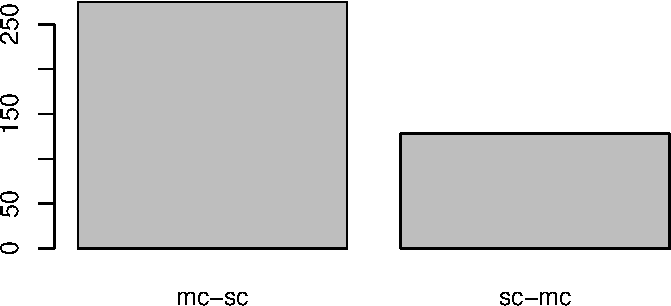
\includegraphics{Categorical_data_files/figure-pdf/unnamed-chunk-10-1.pdf}

\subsection{ggplot2}

\begin{itemize}
\tightlist
\item
  Barplot with \texttt{geom\_bar()} using the raw input data
\end{itemize}

\begin{Shaded}
\begin{Highlighting}[]
\FunctionTok{library}\NormalTok{(tidyverse)}

\FunctionTok{ggplot}\NormalTok{(cl.order, }\FunctionTok{aes}\NormalTok{(}\AttributeTok{x =}\NormalTok{ ORDER)) }\SpecialCharTok{+}
  \FunctionTok{geom\_bar}\NormalTok{()}
\end{Highlighting}
\end{Shaded}

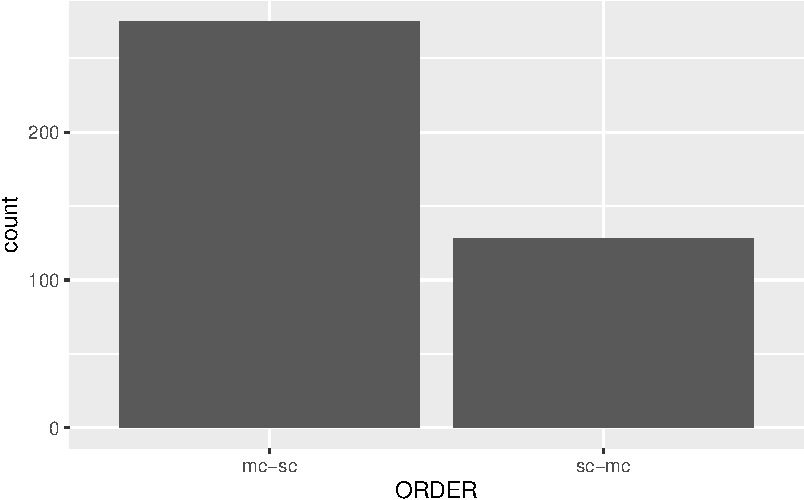
\includegraphics{Categorical_data_files/figure-pdf/unnamed-chunk-11-1.pdf}

\subsection{Two variables}\label{two-variables-1}

\begin{itemize}
\tightlist
\item
  Barplots with the \texttt{fill} argument
\end{itemize}

\subsection{Base R}

\begin{Shaded}
\begin{Highlighting}[]
\FunctionTok{barplot}\NormalTok{(order\_counts2, }
        \AttributeTok{beside =} \ConstantTok{TRUE}\NormalTok{,  }\CommentTok{\# Make bars side{-}by{-}side}
        \AttributeTok{legend =} \ConstantTok{TRUE}\NormalTok{)  }\CommentTok{\# Add a legend}
\end{Highlighting}
\end{Shaded}

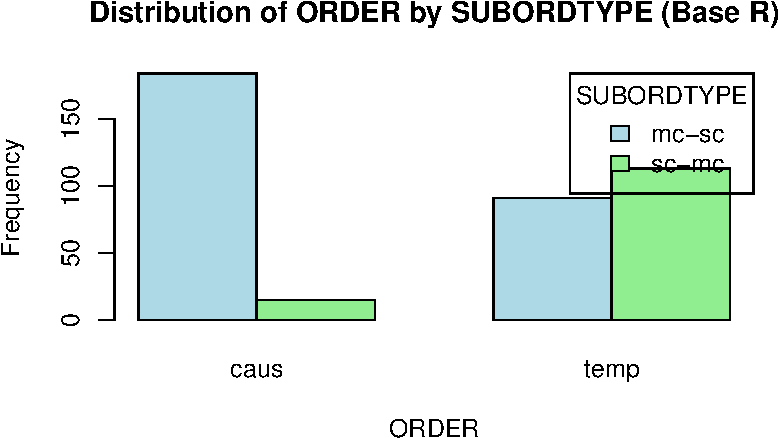
\includegraphics{Categorical_data_files/figure-pdf/unnamed-chunk-12-1.pdf}

\subsection{Base R (fully customised)}

\begin{Shaded}
\begin{Highlighting}[]
\FunctionTok{barplot}\NormalTok{(order\_counts2, }
        \AttributeTok{beside =} \ConstantTok{TRUE}\NormalTok{,  }\CommentTok{\# Make bars dodged (i.e., side by side)}
        \AttributeTok{main =} \StringTok{"Distribution of ORDER by SUBORDTYPE (Base R)"}\NormalTok{, }
        \AttributeTok{xlab =} \StringTok{"ORDER"}\NormalTok{, }
        \AttributeTok{ylab =} \StringTok{"Frequency"}\NormalTok{, }
        \AttributeTok{col =} \FunctionTok{c}\NormalTok{(}\StringTok{"lightblue"}\NormalTok{, }\StringTok{"lightgreen"}\NormalTok{), }\CommentTok{\# Customize colors}
        \AttributeTok{legend =} \ConstantTok{TRUE}\NormalTok{,  }\CommentTok{\# Add a legend}
        \AttributeTok{args.legend =} \FunctionTok{list}\NormalTok{(}\AttributeTok{title =} \StringTok{"SUBORDTYPE"}\NormalTok{, }\AttributeTok{x =} \StringTok{"topright"}\NormalTok{))}
\end{Highlighting}
\end{Shaded}

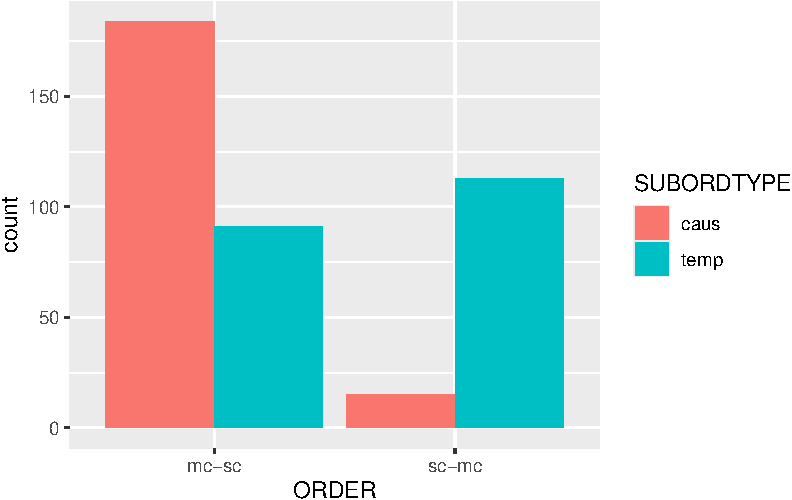
\includegraphics{Categorical_data_files/figure-pdf/unnamed-chunk-13-1.pdf}

\subsection{ggplot2}

\begin{Shaded}
\begin{Highlighting}[]
\FunctionTok{library}\NormalTok{(tidyverse)}

\FunctionTok{ggplot}\NormalTok{(cl.order, }\FunctionTok{aes}\NormalTok{(}\AttributeTok{x =}\NormalTok{ ORDER, }\AttributeTok{fill =}\NormalTok{ SUBORDTYPE)) }\SpecialCharTok{+}
  \FunctionTok{geom\_bar}\NormalTok{(}\AttributeTok{position =} \StringTok{"dodge"}\NormalTok{)}
\end{Highlighting}
\end{Shaded}

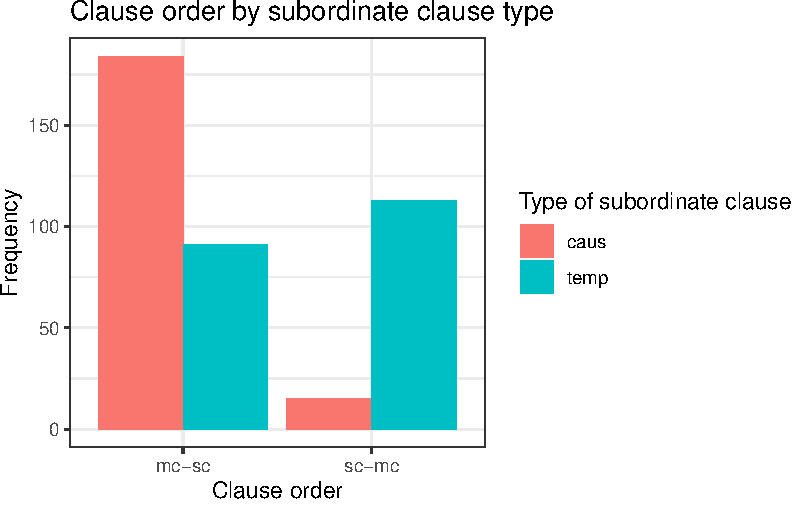
\includegraphics{Categorical_data_files/figure-pdf/unnamed-chunk-14-1.pdf}

\subsection{ggplot2 (fully customised)}

\begin{Shaded}
\begin{Highlighting}[]
\FunctionTok{library}\NormalTok{(tidyverse)}

\FunctionTok{ggplot}\NormalTok{(cl.order, }\FunctionTok{aes}\NormalTok{(}\AttributeTok{x =}\NormalTok{ ORDER, }\AttributeTok{fill =}\NormalTok{ SUBORDTYPE)) }\SpecialCharTok{+}
  \FunctionTok{geom\_bar}\NormalTok{(}\AttributeTok{position =} \StringTok{"dodge"}\NormalTok{) }\SpecialCharTok{+}
  \FunctionTok{labs}\NormalTok{(}
    \AttributeTok{title =} \StringTok{"Clause order by subordinate clause type"}\NormalTok{,}
    \AttributeTok{x =} \StringTok{"Clause order"}\NormalTok{,}
    \AttributeTok{y =} \StringTok{"Frequency"}\NormalTok{,}
    \AttributeTok{fill =} \StringTok{"Type of subordinate clause"}
\NormalTok{  ) }\SpecialCharTok{+}
  \FunctionTok{theme\_bw}\NormalTok{()}
\end{Highlighting}
\end{Shaded}

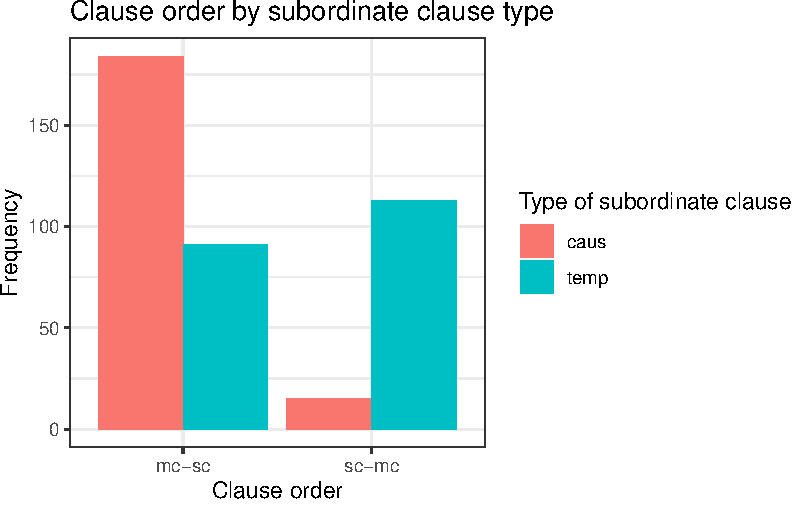
\includegraphics{Categorical_data_files/figure-pdf/unnamed-chunk-15-1.pdf}

\begin{tcolorbox}[enhanced jigsaw, toprule=.15mm, opacitybacktitle=0.6, coltitle=black, arc=.35mm, colback=white, title=\textcolor{quarto-callout-note-color}{\faInfo}\hspace{0.5em}{How do I plot percentages?}, titlerule=0mm, toptitle=1mm, bottomtitle=1mm, breakable, rightrule=.15mm, opacityback=0, bottomrule=.15mm, leftrule=.75mm, colframe=quarto-callout-note-color-frame, left=2mm, colbacktitle=quarto-callout-note-color!10!white]

In Base R, very much the same way as with the raw counts:

\begin{Shaded}
\begin{Highlighting}[]
\FunctionTok{barplot}\NormalTok{(pct1, }
        \AttributeTok{beside =} \ConstantTok{TRUE}\NormalTok{,  }\CommentTok{\# Make bars side{-}by{-}side}
        \AttributeTok{legend =} \ConstantTok{TRUE}\NormalTok{)  }\CommentTok{\# Add a legend}
\end{Highlighting}
\end{Shaded}

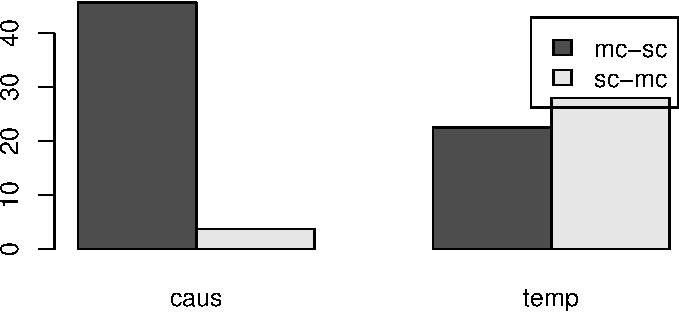
\includegraphics{Categorical_data_files/figure-pdf/unnamed-chunk-16-1.pdf}

In ggplot2, a few tweaks are necessary. In general, ggplot2 only works
with data frames and not with table objects, so we'd have to convert it
to one first:

\begin{Shaded}
\begin{Highlighting}[]
\NormalTok{pct1\_df }\OtherTok{\textless{}{-}} \FunctionTok{as.data.frame}\NormalTok{(pct1)}

\FunctionTok{print}\NormalTok{(pct1\_df)}
\end{Highlighting}
\end{Shaded}

\begin{verbatim}
   Var1 Var2      Freq
1 mc-sc caus 45.657568
2 sc-mc caus  3.722084
3 mc-sc temp 22.580645
4 sc-mc temp 28.039702
\end{verbatim}

Now we can plot the percentages with \texttt{geom\_col()}. This geom (=
`geometric object') allows us to manually specify what should be mapped
onto the y-axis:

\begin{Shaded}
\begin{Highlighting}[]
\FunctionTok{library}\NormalTok{(tidyverse)}

\FunctionTok{ggplot}\NormalTok{(pct1\_df, }\FunctionTok{aes}\NormalTok{(}\AttributeTok{x =}\NormalTok{ Var1, }\AttributeTok{y =}\NormalTok{ Freq, }\AttributeTok{fill =}\NormalTok{ Var2)) }\SpecialCharTok{+}
  \FunctionTok{geom\_col}\NormalTok{(}\AttributeTok{position =} \StringTok{"dodge"}\NormalTok{)}
\end{Highlighting}
\end{Shaded}

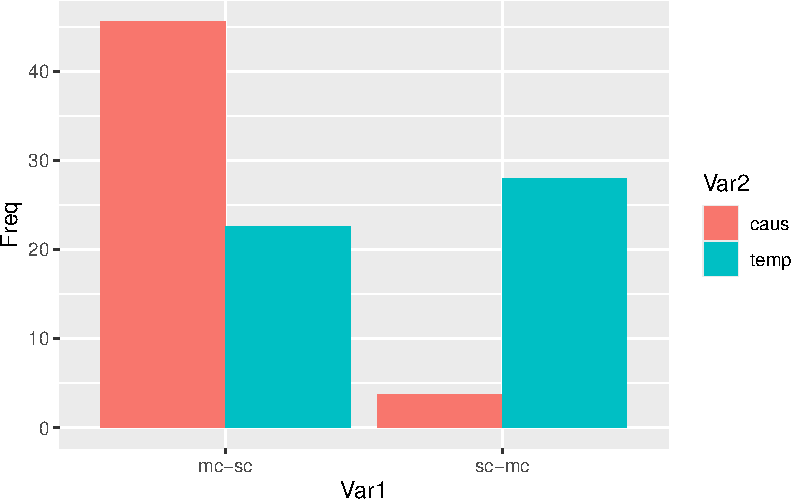
\includegraphics{Categorical_data_files/figure-pdf/unnamed-chunk-18-1.pdf}

\end{tcolorbox}

\section{Exporting tables to MS Word}\label{exporting-tables-to-ms-word}

Publication-ready tables can be generated with the help of the
\texttt{flextable} package. The full guide can be found
\href{https://ardata-fr.github.io/flextable-book/crosstabs.html\#using-tables}{here}.

\begin{Shaded}
\begin{Highlighting}[]
\FunctionTok{library}\NormalTok{(flextable)}
\NormalTok{output\_1 }\OtherTok{\textless{}{-}} \FunctionTok{as\_flextable}\NormalTok{(pct1)}
\FunctionTok{print}\NormalTok{(output\_1)}
\end{Highlighting}
\end{Shaded}

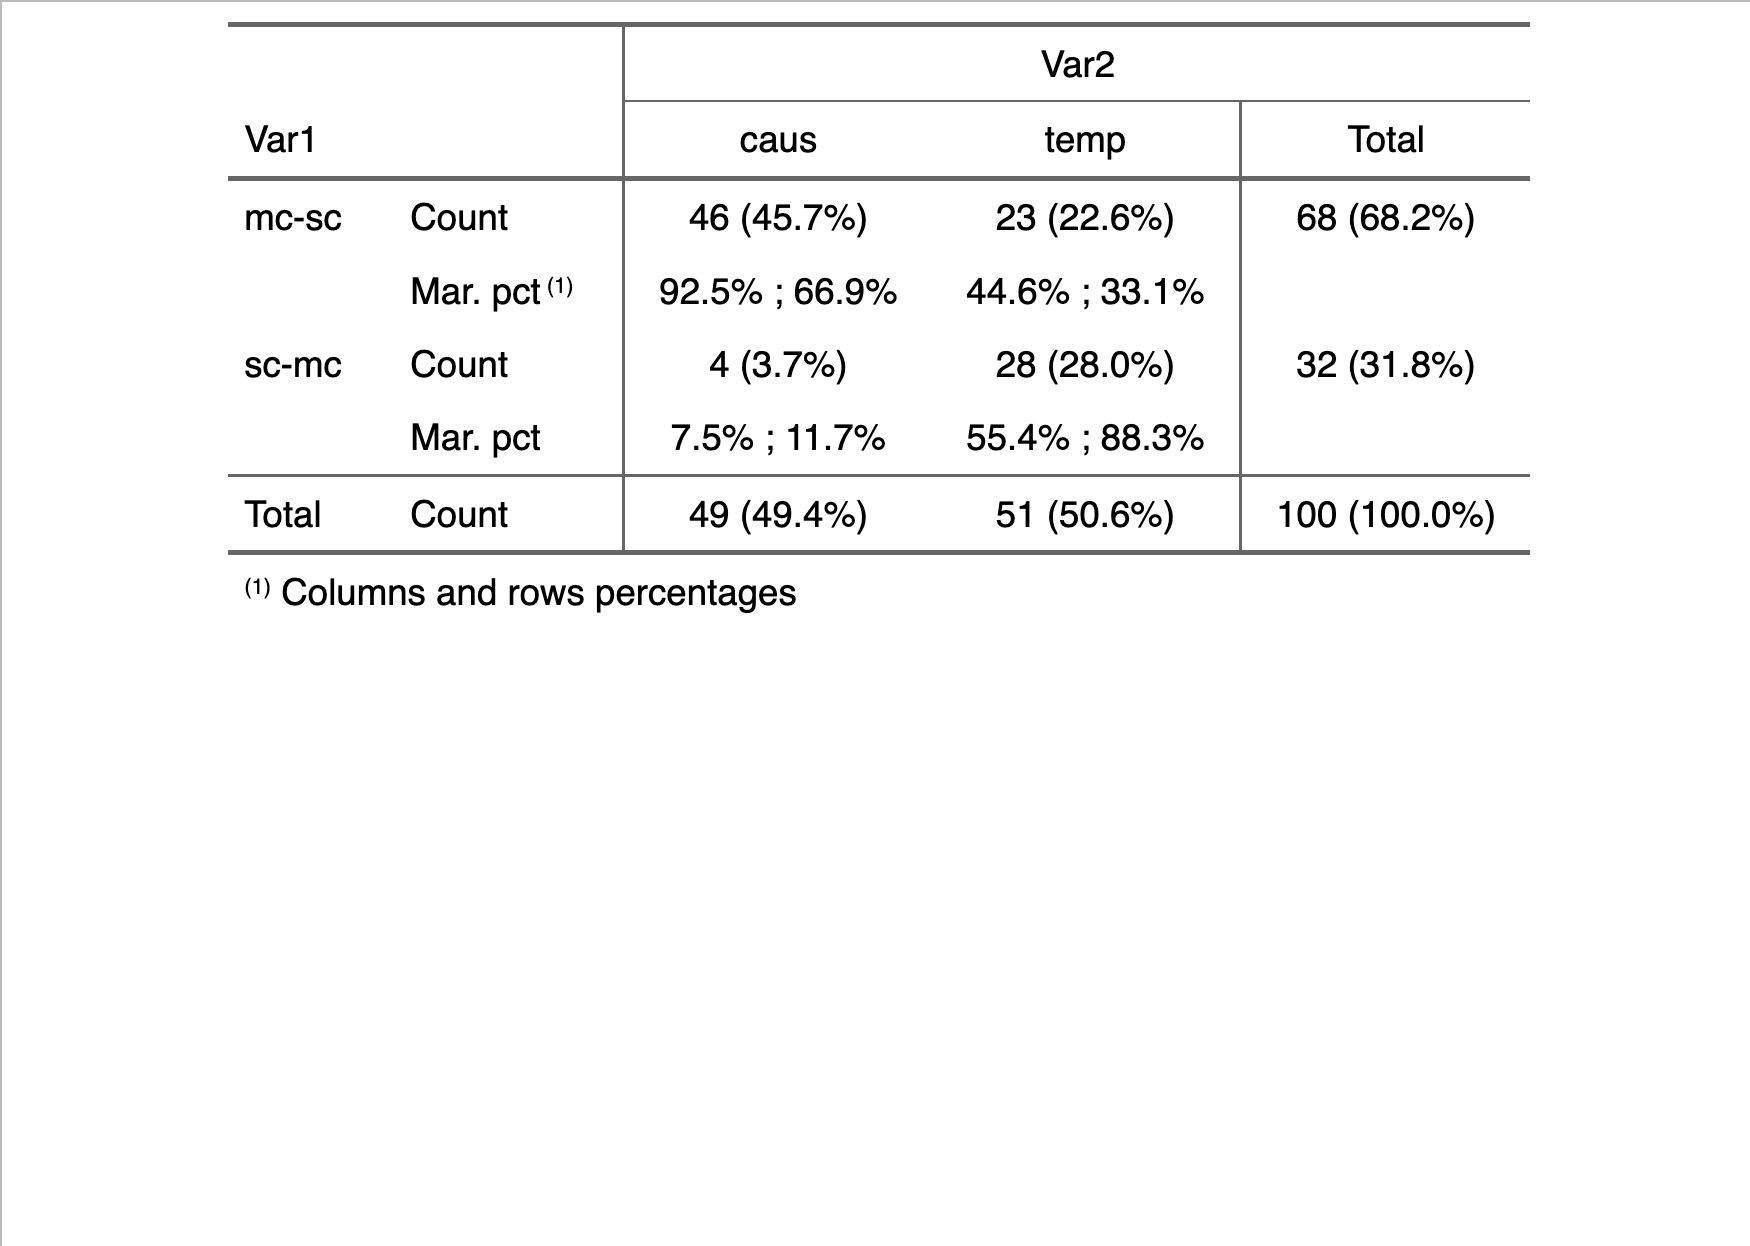
\includegraphics{crosstable_plot1.png}

The \texttt{rempsyc} also provides a simple way of creating beautiful,
export-ready tables. You can find the documentation
\href{https://rempsyc.remi-theriault.com/articles/table}{here}.

\begin{Shaded}
\begin{Highlighting}[]
\FunctionTok{library}\NormalTok{(rempsyc)}

\CommentTok{\# Format table}
\NormalTok{output2 }\OtherTok{\textless{}{-}} \FunctionTok{nice\_table}\NormalTok{(pct1\_df)}

\FunctionTok{print}\NormalTok{(output2)}
\end{Highlighting}
\end{Shaded}

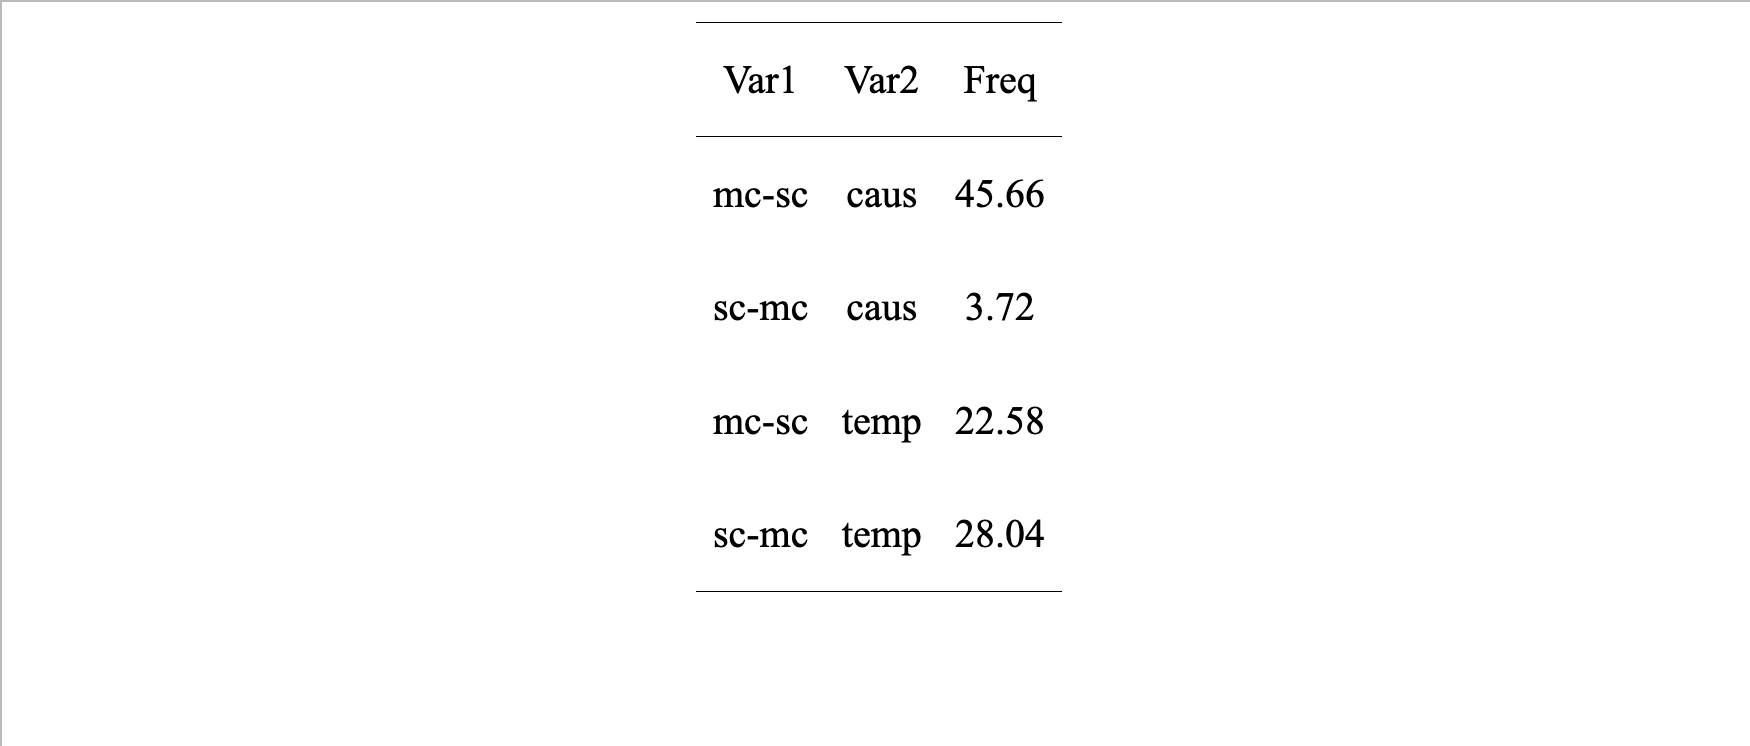
\includegraphics{crosstable_plot2.png}

\begin{Shaded}
\begin{Highlighting}[]
\CommentTok{\# Export to Microsoft Word}
\FunctionTok{print}\NormalTok{(output2, }\AttributeTok{preview =} \StringTok{"docx"}\NormalTok{)}
\end{Highlighting}
\end{Shaded}

\chapter{Continuous data}\label{continuous-data}

\section{Preparation}\label{preparation-4}

We will use the dataset from the previous unit:

\begin{Shaded}
\begin{Highlighting}[]
\CommentTok{\# Libraries}
\FunctionTok{library}\NormalTok{(}\StringTok{"readxl"}\NormalTok{)}
\FunctionTok{library}\NormalTok{(}\StringTok{"tidyverse"}\NormalTok{)}

\CommentTok{\# Load data from working directory}
\NormalTok{cl.order }\OtherTok{\textless{}{-}} \FunctionTok{read\_xlsx}\NormalTok{(}\StringTok{"Paquot\_Larsson\_2020\_data.xlsx"}\NormalTok{)}
\end{Highlighting}
\end{Shaded}

\section{Measures of central
tendency}\label{measures-of-central-tendency}

\subsection{The mean}\label{the-mean}

A useful summary statistic is the arithmetic mean \(\bar{x}\) (cf.
Heumann, Schomaker, and Shalabh 2022: 38). Consider a continuous
variable \(X\) with observations \(x_1, x_2, ..., x_n\) from a sample of
size \(n\). The sample mean \(\bar{x}\) then corresponds to

\[
\bar{x} = \frac{x_1 + x_2 + ... + x_n}{n} \\ = \frac{1}{n}\sum_{i=1}^n{x_i}.
\]

\begin{tcolorbox}[enhanced jigsaw, toprule=.15mm, opacitybacktitle=0.6, coltitle=black, arc=.35mm, colback=white, title=\textcolor{quarto-callout-note-color}{\faInfo}\hspace{0.5em}{Hold on, what does this large Σ symbol mean?}, titlerule=0mm, toptitle=1mm, bottomtitle=1mm, breakable, rightrule=.15mm, opacityback=0, bottomrule=.15mm, leftrule=.75mm, colframe=quarto-callout-note-color-frame, left=2mm, colbacktitle=quarto-callout-note-color!10!white]

The summation symbol \(\sum\) is a concise way to express the sum of a
sequence of numbers. It works like this:

\begin{itemize}
\item
  The expression below the \(\sum\) (e.g., \(i = 1\)) indicates the
  starting value of the index \(i\).
\item
  The number above the \(\sum\) (e.g., \(n\)) is the ending value of the
  index \(i\).
\item
  The expression to the right of the \(\sum\) (e.g., \(x_i\)) is the
  term to be summed.
\end{itemize}

For instance, the expression \(\sum_{i=1}^n{x_i}\) means ``sum the
values of \(x_i\) starting from \(i = 1\) up to \(i = n\).'' In other
words, it adds up the values \(x_1 + x_2 + \dots + x_n\).

\end{tcolorbox}

In R, we can obtain the average value of a numeric vector with the
\texttt{mean()} function. Let's do that for the length of main clauses
found in the \texttt{cl.order} data:

\begin{Shaded}
\begin{Highlighting}[]
\CommentTok{\# Using mean()}
\FunctionTok{mean}\NormalTok{(cl.order}\SpecialCharTok{$}\NormalTok{LEN\_MC)}
\end{Highlighting}
\end{Shaded}

\begin{verbatim}
[1] 9.265509
\end{verbatim}

\begin{tcolorbox}[enhanced jigsaw, toprule=.15mm, opacitybacktitle=0.6, coltitle=black, arc=.35mm, colback=white, title=\textcolor{quarto-callout-tip-color}{\faLightbulb}\hspace{0.5em}{Compute the sample mean by hand}, titlerule=0mm, toptitle=1mm, bottomtitle=1mm, breakable, rightrule=.15mm, opacityback=0, bottomrule=.15mm, leftrule=.75mm, colframe=quarto-callout-tip-color-frame, left=2mm, colbacktitle=quarto-callout-tip-color!10!white]

\begin{Shaded}
\begin{Highlighting}[]
\NormalTok{mean }\OtherTok{\textless{}{-}} \DecValTok{1}\SpecialCharTok{/}\FunctionTok{length}\NormalTok{(cl.order}\SpecialCharTok{$}\NormalTok{LEN\_MC) }\SpecialCharTok{*} \FunctionTok{sum}\NormalTok{(cl.order}\SpecialCharTok{$}\NormalTok{LEN\_MC)}
\end{Highlighting}
\end{Shaded}

\end{tcolorbox}

The output returned by this function provides a one-value summary of all
observations contained in \texttt{LEN\_MC}. How could we visualise it?

First, let's create a histogram of \texttt{LEN\_MC}. Histograms
summarise how often certain values occur in a continuous variable. The
blue line indicates the sample mean. Alternatively, you can use a
density plot to represent the probability of encountering a specific
value in the data.

\subsection{Histogram (ggplot2)}

\begin{Shaded}
\begin{Highlighting}[]
\CommentTok{\# Plot distribution of LEN\_MC}
\NormalTok{cl.length.hist }\OtherTok{\textless{}{-}} \FunctionTok{ggplot}\NormalTok{(cl.order, }\FunctionTok{aes}\NormalTok{(}\AttributeTok{x =}\NormalTok{ LEN\_MC)) }\SpecialCharTok{+}
                  \FunctionTok{geom\_histogram}\NormalTok{(}\AttributeTok{binwidth =} \DecValTok{2}\NormalTok{)}

\NormalTok{cl.length.hist }\SpecialCharTok{+}
  \CommentTok{\# Add mean}
  \FunctionTok{geom\_vline}\NormalTok{(}\FunctionTok{aes}\NormalTok{(}\AttributeTok{xintercept =} \FunctionTok{mean}\NormalTok{(LEN\_MC)),}
             \AttributeTok{color =} \StringTok{"steelblue"}\NormalTok{,}
             \AttributeTok{linewidth =} \DecValTok{1}\NormalTok{) }\SpecialCharTok{+}
  \FunctionTok{theme\_classic}\NormalTok{()}
\end{Highlighting}
\end{Shaded}

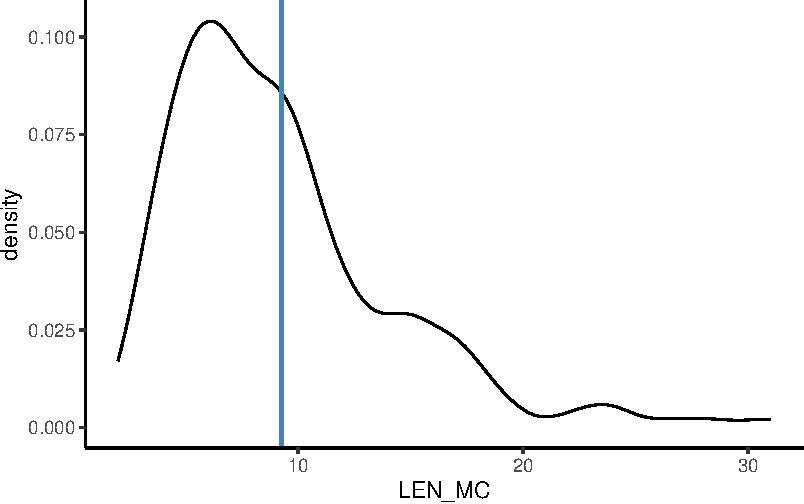
\includegraphics{Summary_statistics_files/figure-pdf/unnamed-chunk-4-1.pdf}

\subsection{Density plot (ggplot2)}

\begin{Shaded}
\begin{Highlighting}[]
\CommentTok{\# Plot distribution of LEN\_MC}
\NormalTok{cl.length.dens }\OtherTok{\textless{}{-}} \FunctionTok{ggplot}\NormalTok{(cl.order, }\FunctionTok{aes}\NormalTok{(}\AttributeTok{x =}\NormalTok{ LEN\_MC)) }\SpecialCharTok{+}
                  \FunctionTok{geom\_density}\NormalTok{()}

\NormalTok{cl.length.dens }\SpecialCharTok{+}
  \CommentTok{\# Add mean}
  \FunctionTok{geom\_vline}\NormalTok{(}\FunctionTok{aes}\NormalTok{(}\AttributeTok{xintercept =} \FunctionTok{mean}\NormalTok{(LEN\_MC)),}
             \AttributeTok{color =} \StringTok{"steelblue"}\NormalTok{,}
             \AttributeTok{linewidth =} \DecValTok{1}\NormalTok{) }\SpecialCharTok{+}
  \FunctionTok{theme\_classic}\NormalTok{()}
\end{Highlighting}
\end{Shaded}

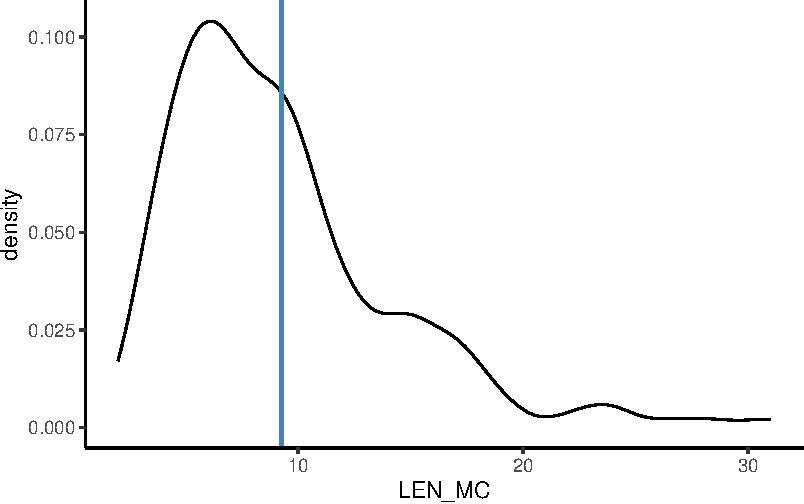
\includegraphics{Summary_statistics_files/figure-pdf/unnamed-chunk-5-1.pdf}

\subsection{Histogram (Base R)}

\begin{Shaded}
\begin{Highlighting}[]
\FunctionTok{hist}\NormalTok{(cl.order}\SpecialCharTok{$}\NormalTok{LEN\_MC)}
  \FunctionTok{abline}\NormalTok{(}\AttributeTok{v=}\FunctionTok{mean}\NormalTok{(cl.order}\SpecialCharTok{$}\NormalTok{LEN\_MC),}\AttributeTok{lwd=}\DecValTok{3}\NormalTok{, }\AttributeTok{col =} \StringTok{"steelblue"}\NormalTok{)}
\end{Highlighting}
\end{Shaded}

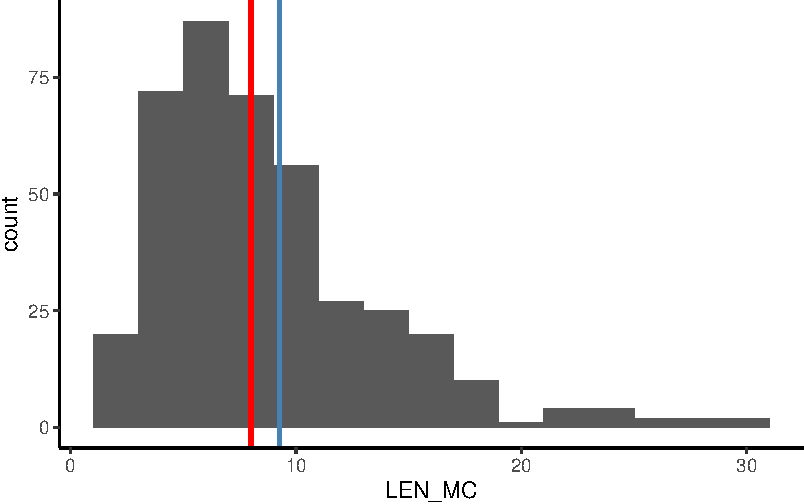
\includegraphics{Summary_statistics_files/figure-pdf/unnamed-chunk-6-1.pdf}

\subsection{Density plot (Base R)}

\begin{Shaded}
\begin{Highlighting}[]
\FunctionTok{plot}\NormalTok{(}\FunctionTok{density}\NormalTok{(cl.order}\SpecialCharTok{$}\NormalTok{LEN\_MC))}
  \FunctionTok{abline}\NormalTok{(}\AttributeTok{v=}\FunctionTok{mean}\NormalTok{(cl.order}\SpecialCharTok{$}\NormalTok{LEN\_MC),}\AttributeTok{lwd=}\DecValTok{3}\NormalTok{, }\AttributeTok{col =} \StringTok{"steelblue"}\NormalTok{)}
\end{Highlighting}
\end{Shaded}

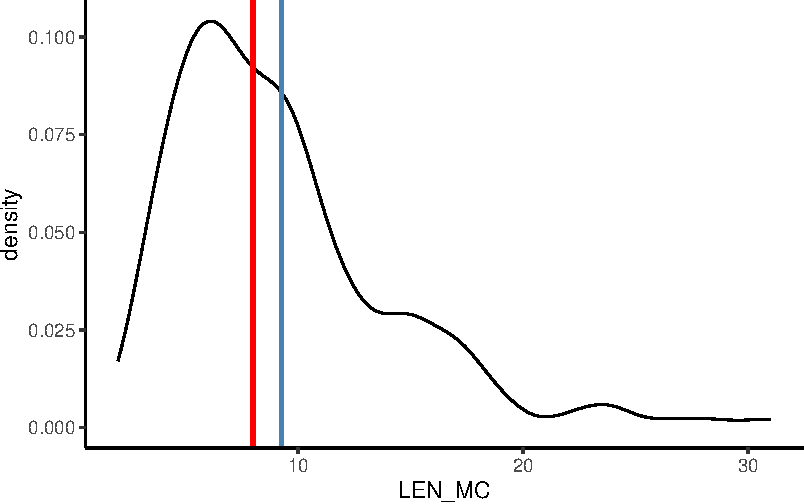
\includegraphics{Summary_statistics_files/figure-pdf/unnamed-chunk-7-1.pdf}

\subsection{The median}\label{the-median}

The \texttt{median()} function computes the ``the halfway point of the
data (50\% of the data are above the median; 50\% of the data are
below'' (Winter 2020: 58).

\[
\tilde{x}_{0.5} = 
\begin{cases}
x_{((n+1)/2)} & \text{if } n \text{ is odd.} \\
\frac{1}{2}(x_{n/2}+x_{(n/2+1)}) & \text{if } n \text{ is even.}
\end{cases} 
\]

\begin{Shaded}
\begin{Highlighting}[]
\CommentTok{\# Using median()}
\FunctionTok{median}\NormalTok{(cl.order}\SpecialCharTok{$}\NormalTok{LEN\_MC)}
\end{Highlighting}
\end{Shaded}

\begin{verbatim}
[1] 8
\end{verbatim}

\begin{tcolorbox}[enhanced jigsaw, toprule=.15mm, opacitybacktitle=0.6, coltitle=black, arc=.35mm, colback=white, title=\textcolor{quarto-callout-tip-color}{\faLightbulb}\hspace{0.5em}{Compute the median by hand}, titlerule=0mm, toptitle=1mm, bottomtitle=1mm, breakable, rightrule=.15mm, opacityback=0, bottomrule=.15mm, leftrule=.75mm, colframe=quarto-callout-tip-color-frame, left=2mm, colbacktitle=quarto-callout-tip-color!10!white]

\begin{Shaded}
\begin{Highlighting}[]
\NormalTok{sample\_sorted }\OtherTok{\textless{}{-}} \FunctionTok{sort}\NormalTok{(cl.order}\SpecialCharTok{$}\NormalTok{LEN\_MC) }\CommentTok{\# sort values in ascending order}

\NormalTok{n }\OtherTok{\textless{}{-}} \FunctionTok{length}\NormalTok{(cl.order}\SpecialCharTok{$}\NormalTok{LEN\_MC) }\CommentTok{\# sample size is 403 (odd number!)}

\NormalTok{median }\OtherTok{\textless{}{-}}\NormalTok{ sample\_sorted[(n }\SpecialCharTok{+} \DecValTok{1}\NormalTok{) }\SpecialCharTok{\%/\%} \DecValTok{2}\NormalTok{] }\CommentTok{\# compute median}
\end{Highlighting}
\end{Shaded}

\end{tcolorbox}

The median of \texttt{LEN\_MC} is represented by the red vertical line.

\subsection{Histogram (ggplot2)}

\begin{Shaded}
\begin{Highlighting}[]
\NormalTok{cl.length.hist }\SpecialCharTok{+}
  \CommentTok{\# Add mean}
  \FunctionTok{geom\_vline}\NormalTok{(}\FunctionTok{aes}\NormalTok{(}\AttributeTok{xintercept =} \FunctionTok{mean}\NormalTok{(LEN\_MC)), }\AttributeTok{color =} \StringTok{"steelblue"}\NormalTok{, }\AttributeTok{linewidth =} \DecValTok{1}\NormalTok{) }\SpecialCharTok{+}
  \CommentTok{\# Add median}
  \FunctionTok{geom\_vline}\NormalTok{(}\FunctionTok{aes}\NormalTok{(}\AttributeTok{xintercept =} \FunctionTok{median}\NormalTok{(LEN\_MC)), }\AttributeTok{color =} \StringTok{"red"}\NormalTok{, }\AttributeTok{linewidth =} \DecValTok{1}\NormalTok{) }\SpecialCharTok{+}
  \FunctionTok{theme\_classic}\NormalTok{()}
\end{Highlighting}
\end{Shaded}

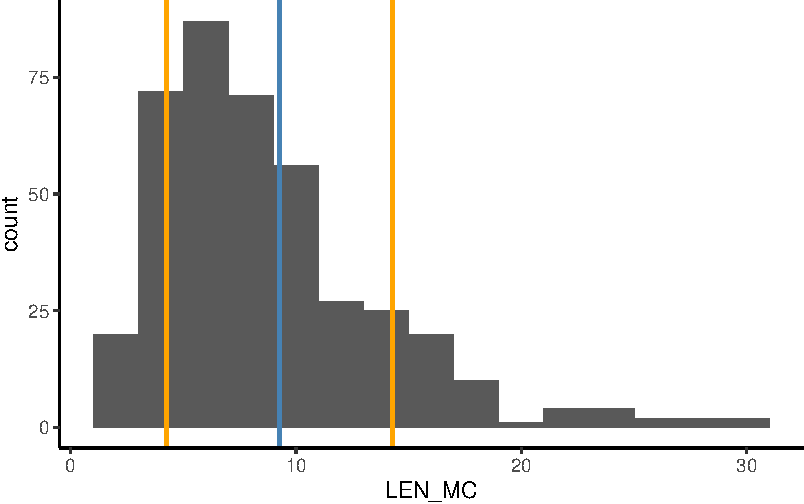
\includegraphics{Summary_statistics_files/figure-pdf/unnamed-chunk-10-1.pdf}

\subsection{Density plot (ggplot2)}

\begin{Shaded}
\begin{Highlighting}[]
\NormalTok{cl.length.dens }\SpecialCharTok{+}
  \CommentTok{\# Add mean}
  \FunctionTok{geom\_vline}\NormalTok{(}\FunctionTok{aes}\NormalTok{(}\AttributeTok{xintercept =} \FunctionTok{mean}\NormalTok{(LEN\_MC)), }\AttributeTok{color =} \StringTok{"steelblue"}\NormalTok{, }\AttributeTok{linewidth =} \DecValTok{1}\NormalTok{) }\SpecialCharTok{+}
  \CommentTok{\# Add median}
  \FunctionTok{geom\_vline}\NormalTok{(}\FunctionTok{aes}\NormalTok{(}\AttributeTok{xintercept =} \FunctionTok{median}\NormalTok{(LEN\_MC)), }\AttributeTok{color =} \StringTok{"red"}\NormalTok{, }\AttributeTok{linewidth =} \DecValTok{1}\NormalTok{) }\SpecialCharTok{+}
  \FunctionTok{theme\_classic}\NormalTok{()}
\end{Highlighting}
\end{Shaded}

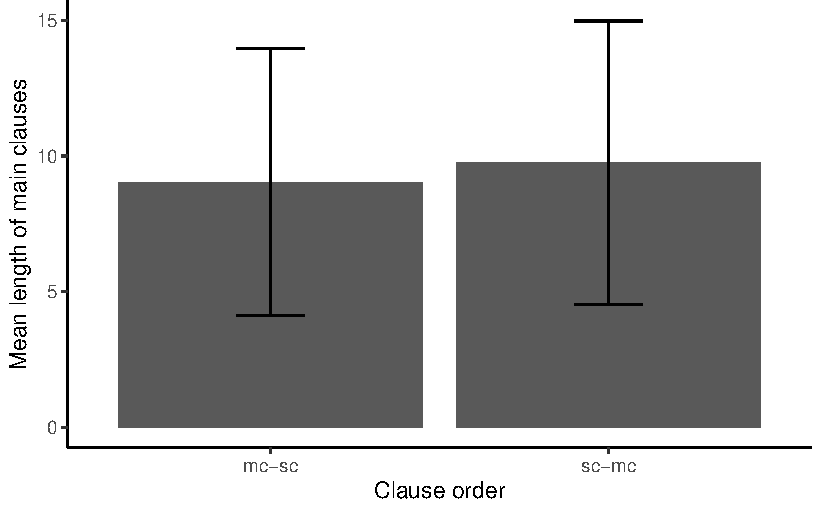
\includegraphics{Summary_statistics_files/figure-pdf/unnamed-chunk-11-1.pdf}

\subsection{Histogram (Base R)}

\begin{Shaded}
\begin{Highlighting}[]
\FunctionTok{hist}\NormalTok{(cl.order}\SpecialCharTok{$}\NormalTok{LEN\_MC)}
  \FunctionTok{abline}\NormalTok{(}\AttributeTok{v=}\FunctionTok{mean}\NormalTok{(cl.order}\SpecialCharTok{$}\NormalTok{LEN\_MC),}\AttributeTok{lwd=}\DecValTok{3}\NormalTok{, }\AttributeTok{col =} \StringTok{"steelblue"}\NormalTok{)}
  \FunctionTok{abline}\NormalTok{(}\AttributeTok{v=}\FunctionTok{median}\NormalTok{(cl.order}\SpecialCharTok{$}\NormalTok{LEN\_MC),}\AttributeTok{lwd=}\DecValTok{3}\NormalTok{, }\AttributeTok{col =} \StringTok{"red"}\NormalTok{)}
\end{Highlighting}
\end{Shaded}

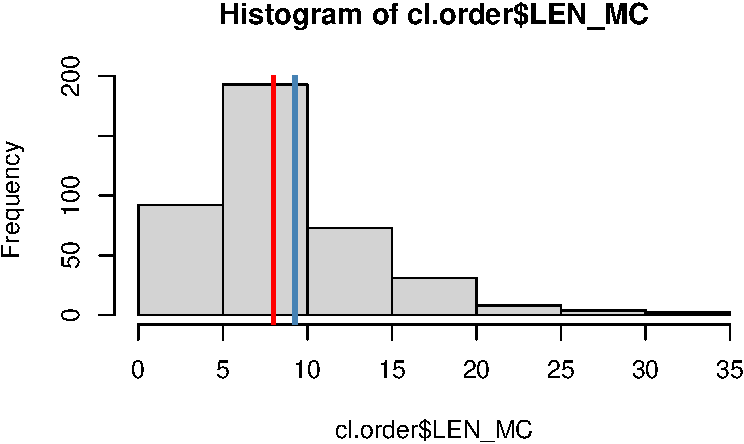
\includegraphics{Summary_statistics_files/figure-pdf/unnamed-chunk-12-1.pdf}

\subsection{Density plot (Base R)}

\begin{Shaded}
\begin{Highlighting}[]
\FunctionTok{plot}\NormalTok{(}\FunctionTok{density}\NormalTok{(cl.order}\SpecialCharTok{$}\NormalTok{LEN\_MC))}
  \FunctionTok{abline}\NormalTok{(}\AttributeTok{v=}\FunctionTok{mean}\NormalTok{(cl.order}\SpecialCharTok{$}\NormalTok{LEN\_MC),}\AttributeTok{lwd=}\DecValTok{3}\NormalTok{, }\AttributeTok{col =} \StringTok{"steelblue"}\NormalTok{)}
  \FunctionTok{abline}\NormalTok{(}\AttributeTok{v=}\FunctionTok{mean}\NormalTok{(cl.order}\SpecialCharTok{$}\NormalTok{LEN\_MC),}\AttributeTok{lwd=}\DecValTok{3}\NormalTok{, }\AttributeTok{col =} \StringTok{"red"}\NormalTok{)}
\end{Highlighting}
\end{Shaded}

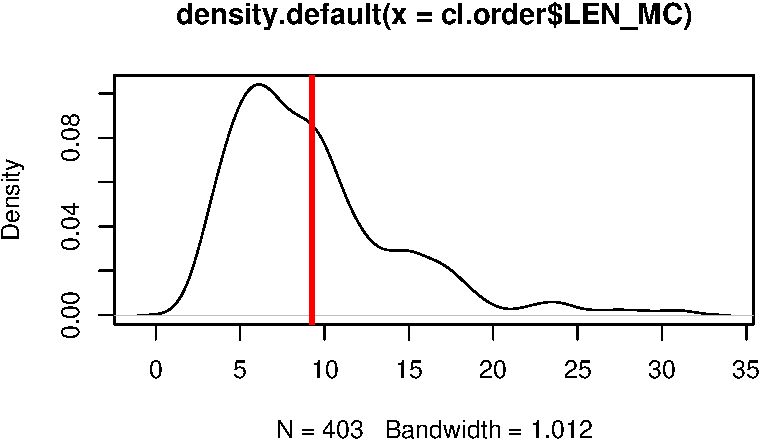
\includegraphics{Summary_statistics_files/figure-pdf/unnamed-chunk-13-1.pdf}

\subsection{Sample variance and standard
deviation}\label{sample-variance-and-standard-deviation}

In order to assess how well the mean represents the data, it is
instructive to compute the \textbf{variance} \texttt{var()} and the
\textbf{standard deviation} \texttt{sd()} for a sample.

The sample variance \(s^2\) is defined as

\[s^2 = \frac{1}{n}\sum_{i=1}^n{(x_i - \bar{x})^2}. \]

In other words, it stands for the average squared deviation of all
observations from the sample mean.

\begin{Shaded}
\begin{Highlighting}[]
\CommentTok{\# Using var()}
\FunctionTok{var}\NormalTok{(cl.order}\SpecialCharTok{$}\NormalTok{LEN\_MC)}
\end{Highlighting}
\end{Shaded}

\begin{verbatim}
[1] 25.12585
\end{verbatim}

\begin{tcolorbox}[enhanced jigsaw, toprule=.15mm, opacitybacktitle=0.6, coltitle=black, arc=.35mm, colback=white, title=\textcolor{quarto-callout-tip-color}{\faLightbulb}\hspace{0.5em}{Compute the sample variance by hand}, titlerule=0mm, toptitle=1mm, bottomtitle=1mm, breakable, rightrule=.15mm, opacityback=0, bottomrule=.15mm, leftrule=.75mm, colframe=quarto-callout-tip-color-frame, left=2mm, colbacktitle=quarto-callout-tip-color!10!white]

\begin{Shaded}
\begin{Highlighting}[]
\CommentTok{\# Define sample}
\NormalTok{sample\_data }\OtherTok{\textless{}{-}}\NormalTok{ cl.order}\SpecialCharTok{$}\NormalTok{LEN\_MC}

\CommentTok{\# Calculate the sample standard deviation}
\NormalTok{var }\OtherTok{\textless{}{-}} \DecValTok{1} \SpecialCharTok{/} \FunctionTok{length}\NormalTok{(sample\_data) }\SpecialCharTok{*} \FunctionTok{sum}\NormalTok{((sample\_data }\SpecialCharTok{{-}} \FunctionTok{mean}\NormalTok{(sample\_data))}\SpecialCharTok{\^{}}\DecValTok{2}\NormalTok{) }\CommentTok{\# formula above}

\CommentTok{\# Note that R\textquotesingle{}s var() function applies an additional bias correction measure:}
\NormalTok{var\_corrected }\OtherTok{\textless{}{-}} \DecValTok{1} \SpecialCharTok{/}\NormalTok{ (}\FunctionTok{length}\NormalTok{(sample\_data) }\SpecialCharTok{{-}} \DecValTok{1}\NormalTok{) }\SpecialCharTok{*} \FunctionTok{sum}\NormalTok{((sample\_data }\SpecialCharTok{{-}} \FunctionTok{mean}\NormalTok{(sample\_data))}\SpecialCharTok{\^{}}\DecValTok{2}\NormalTok{) }\CommentTok{\# equivalent to var()}
\end{Highlighting}
\end{Shaded}

\end{tcolorbox}

Correspondingly, the standard deviation of the mean is the square root
of the variance (cf. Heumann, Schomaker, and Shalabh 2022: 51-2).

\[ s = \sqrt{\frac{1}{n}\sum_{i=1}^n{(x_i - \bar{x})^2}} \]

\begin{Shaded}
\begin{Highlighting}[]
\CommentTok{\# Using sd()}
\FunctionTok{sd}\NormalTok{(cl.order}\SpecialCharTok{$}\NormalTok{LEN\_MC)}
\end{Highlighting}
\end{Shaded}

\begin{verbatim}
[1] 5.012569
\end{verbatim}

\begin{Shaded}
\begin{Highlighting}[]
\CommentTok{\# or by hand:}

\NormalTok{sample\_data }\OtherTok{\textless{}{-}}\NormalTok{ cl.order}\SpecialCharTok{$}\NormalTok{LEN\_MC}
\end{Highlighting}
\end{Shaded}

\begin{tcolorbox}[enhanced jigsaw, toprule=.15mm, opacitybacktitle=0.6, coltitle=black, arc=.35mm, colback=white, title=\textcolor{quarto-callout-tip-color}{\faLightbulb}\hspace{0.5em}{Compute the sample standard deviation by hand}, titlerule=0mm, toptitle=1mm, bottomtitle=1mm, breakable, rightrule=.15mm, opacityback=0, bottomrule=.15mm, leftrule=.75mm, colframe=quarto-callout-tip-color-frame, left=2mm, colbacktitle=quarto-callout-tip-color!10!white]

\begin{Shaded}
\begin{Highlighting}[]
\NormalTok{sd }\OtherTok{\textless{}{-}} \FunctionTok{sqrt}\NormalTok{(}\DecValTok{1} \SpecialCharTok{/}\NormalTok{ (}\FunctionTok{length}\NormalTok{(sample\_data) }\SpecialCharTok{{-}} \DecValTok{1}\NormalTok{)}\SpecialCharTok{*} \FunctionTok{sum}\NormalTok{((sample\_data }\SpecialCharTok{{-}} \FunctionTok{mean}\NormalTok{(sample\_data))}\SpecialCharTok{\^{}}\DecValTok{2}\NormalTok{))}
\end{Highlighting}
\end{Shaded}

\end{tcolorbox}

\textbf{Visualisation}:

\subsubsection{Example 1}

\begin{Shaded}
\begin{Highlighting}[]
\NormalTok{cl.length.hist }\SpecialCharTok{+}
  \CommentTok{\# Add verticle line for the mean}
  \FunctionTok{geom\_vline}\NormalTok{(}\FunctionTok{aes}\NormalTok{(}\AttributeTok{xintercept =} \FunctionTok{mean}\NormalTok{(LEN\_MC)), }\AttributeTok{color =} \StringTok{"steelblue"}\NormalTok{, }\AttributeTok{linewidth =} \DecValTok{1}\NormalTok{) }\SpecialCharTok{+}
  \CommentTok{\# Add {-}1sd}
  \FunctionTok{geom\_vline}\NormalTok{(}\FunctionTok{aes}\NormalTok{(}\AttributeTok{xintercept =} \FunctionTok{mean}\NormalTok{(LEN\_MC) }\SpecialCharTok{{-}} \FunctionTok{sd}\NormalTok{(LEN\_MC)), }\AttributeTok{color =} \StringTok{"orange"}\NormalTok{, }\AttributeTok{linewidth =} \DecValTok{1}\NormalTok{) }\SpecialCharTok{+}
  \CommentTok{\# Add +1sd}
  \FunctionTok{geom\_vline}\NormalTok{(}\FunctionTok{aes}\NormalTok{(}\AttributeTok{xintercept =} \FunctionTok{mean}\NormalTok{(LEN\_MC) }\SpecialCharTok{+} \FunctionTok{sd}\NormalTok{(LEN\_MC)), }\AttributeTok{color =} \StringTok{"orange"}\NormalTok{, }\AttributeTok{linewidth =} \DecValTok{1}\NormalTok{) }\SpecialCharTok{+}
  \FunctionTok{theme\_classic}\NormalTok{()}
\end{Highlighting}
\end{Shaded}

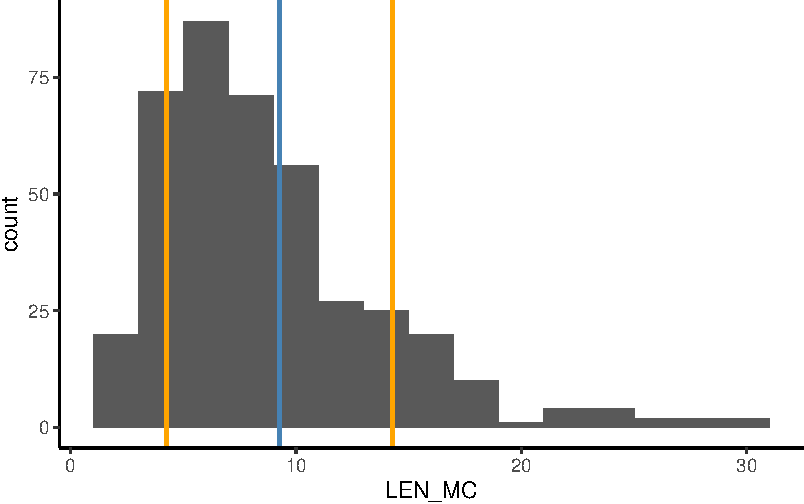
\includegraphics{Summary_statistics_files/figure-pdf/unnamed-chunk-18-1.pdf}

\subsubsection{Example 2}

\begin{Shaded}
\begin{Highlighting}[]
\CommentTok{\# Create data frame with mean and sd for each clause ORDER}

\NormalTok{cl.order }\SpecialCharTok{\%\textgreater{}\%} 
  \CommentTok{\# Select variables of interest}
  \FunctionTok{select}\NormalTok{(ORDER, LEN\_MC) }\SpecialCharTok{\%\textgreater{}\%} 
  \CommentTok{\# Group results of following operations by ORDER}
  \FunctionTok{group\_by}\NormalTok{(ORDER) }\SpecialCharTok{\%\textgreater{}\%} 
    \CommentTok{\# Create grouped summary of mean and sd for each ORDER}
    \FunctionTok{summarise}\NormalTok{(}\AttributeTok{mean =} \FunctionTok{mean}\NormalTok{(LEN\_MC),}
                \AttributeTok{sd =} \FunctionTok{sd}\NormalTok{(LEN\_MC)) }\OtherTok{{-}\textgreater{}}\NormalTok{ cl\_mean\_sd; cl\_mean\_sd}
\end{Highlighting}
\end{Shaded}

\begin{verbatim}
# A tibble: 2 x 3
  ORDER  mean    sd
  <chr> <dbl> <dbl>
1 mc-sc  9.04  4.91
2 sc-mc  9.75  5.22
\end{verbatim}

\begin{Shaded}
\begin{Highlighting}[]
\CommentTok{\# Plot results }

\FunctionTok{ggplot}\NormalTok{(cl\_mean\_sd, }\FunctionTok{aes}\NormalTok{(}\AttributeTok{x =}\NormalTok{ ORDER, }\AttributeTok{y =}\NormalTok{ mean)) }\SpecialCharTok{+}
  \CommentTok{\# Barplot with a specific variable mapped onto y{-}axis}
  \FunctionTok{geom\_col}\NormalTok{() }\SpecialCharTok{+}
  \CommentTok{\# Add mean and standard deviation to the plot}
  \FunctionTok{geom\_errorbar}\NormalTok{(}\FunctionTok{aes}\NormalTok{(}\AttributeTok{x =}\NormalTok{ ORDER,}
                    \AttributeTok{ymin =}\NormalTok{ mean}\SpecialCharTok{{-}}\NormalTok{sd,}
                    \AttributeTok{ymax =}\NormalTok{ mean}\SpecialCharTok{+}\NormalTok{sd), }\AttributeTok{width =}\NormalTok{ .}\DecValTok{2}\NormalTok{) }\SpecialCharTok{+}
  \FunctionTok{theme\_classic}\NormalTok{() }\SpecialCharTok{+}
  \FunctionTok{labs}\NormalTok{(}\AttributeTok{y =} \StringTok{"Mean length of main clauses"}\NormalTok{, }\AttributeTok{x =} \StringTok{"Clause order"}\NormalTok{)}
\end{Highlighting}
\end{Shaded}

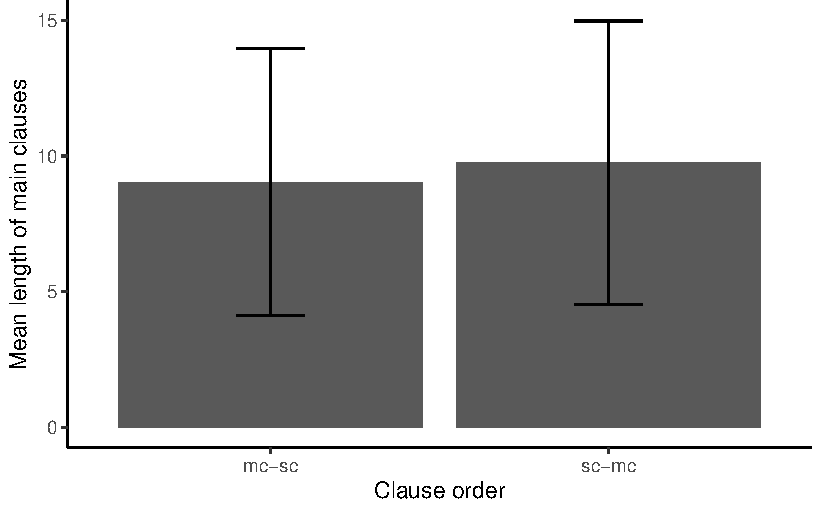
\includegraphics{Summary_statistics_files/figure-pdf/unnamed-chunk-19-1.pdf}

\subsection{Quantiles}\label{quantiles}

While \texttt{median()} divides the data into two equal sets (i.e., two
50\% quantiles), the \texttt{quantile()} function makes it possible to
partition the data further.

\begin{Shaded}
\begin{Highlighting}[]
\FunctionTok{quantile}\NormalTok{(cl.order}\SpecialCharTok{$}\NormalTok{LEN\_MC)}
\end{Highlighting}
\end{Shaded}

\begin{verbatim}
  0%  25%  50%  75% 100% 
   2    6    8   11   31 
\end{verbatim}

\texttt{quantile(x,\ 0)} and \texttt{quantile(x,\ 1)} thus show the
minimum and maximum values, respectively.

\begin{Shaded}
\begin{Highlighting}[]
\FunctionTok{quantile}\NormalTok{(cl.order}\SpecialCharTok{$}\NormalTok{LEN\_MC, }\DecValTok{0}\NormalTok{)}
\end{Highlighting}
\end{Shaded}

\begin{verbatim}
0% 
 2 
\end{verbatim}

\begin{Shaded}
\begin{Highlighting}[]
\FunctionTok{quantile}\NormalTok{(cl.order}\SpecialCharTok{$}\NormalTok{LEN\_MC, }\DecValTok{1}\NormalTok{)}
\end{Highlighting}
\end{Shaded}

\begin{verbatim}
100% 
  31 
\end{verbatim}

\subsection{Quartiles and boxplots}\label{quartiles-and-boxplots}

Consider the distribution of clause length by clause order:

\subsubsection{Boxplot (Base R)}

\begin{Shaded}
\begin{Highlighting}[]
\FunctionTok{boxplot}\NormalTok{(LEN\_MC }\SpecialCharTok{\textasciitilde{}}\NormalTok{ ORDER, cl.order)}
\end{Highlighting}
\end{Shaded}

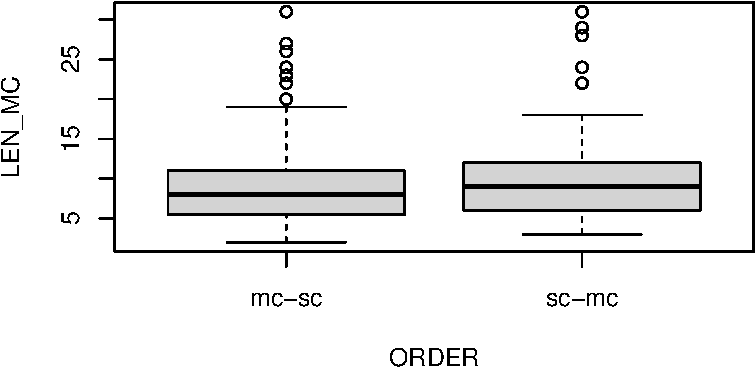
\includegraphics{Summary_statistics_files/figure-pdf/unnamed-chunk-22-1.pdf}

\subsubsection{Boxplot (ggplot2)}

\begin{Shaded}
\begin{Highlighting}[]
\FunctionTok{ggplot}\NormalTok{(cl.order, }\FunctionTok{aes}\NormalTok{(}\AttributeTok{x =}\NormalTok{ ORDER, }\AttributeTok{y =}\NormalTok{ LEN\_MC)) }\SpecialCharTok{+}
  \FunctionTok{geom\_boxplot}\NormalTok{() }\SpecialCharTok{+}
  \FunctionTok{theme\_classic}\NormalTok{()}
\end{Highlighting}
\end{Shaded}

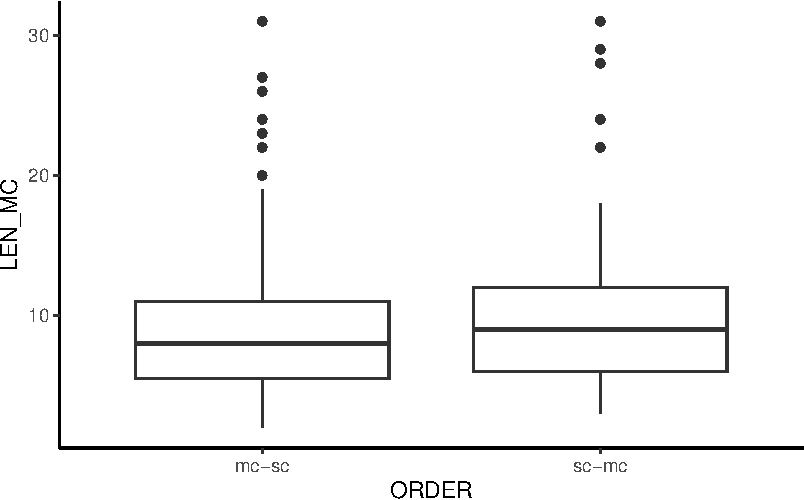
\includegraphics{Summary_statistics_files/figure-pdf/unnamed-chunk-23-1.pdf}

Compare it to the corresponding rotated density plot:

\begin{Shaded}
\begin{Highlighting}[]
\FunctionTok{ggplot}\NormalTok{(cl.order, }\FunctionTok{aes}\NormalTok{(}\AttributeTok{x =}\NormalTok{ LEN\_MC, }\AttributeTok{fill =}\NormalTok{ ORDER)) }\SpecialCharTok{+}
  \FunctionTok{geom\_density}\NormalTok{(}\AttributeTok{alpha =} \FloatTok{0.5}\NormalTok{) }\SpecialCharTok{+}
  \FunctionTok{coord\_flip}\NormalTok{() }\SpecialCharTok{+}
  \FunctionTok{theme\_classic}\NormalTok{()}
\end{Highlighting}
\end{Shaded}

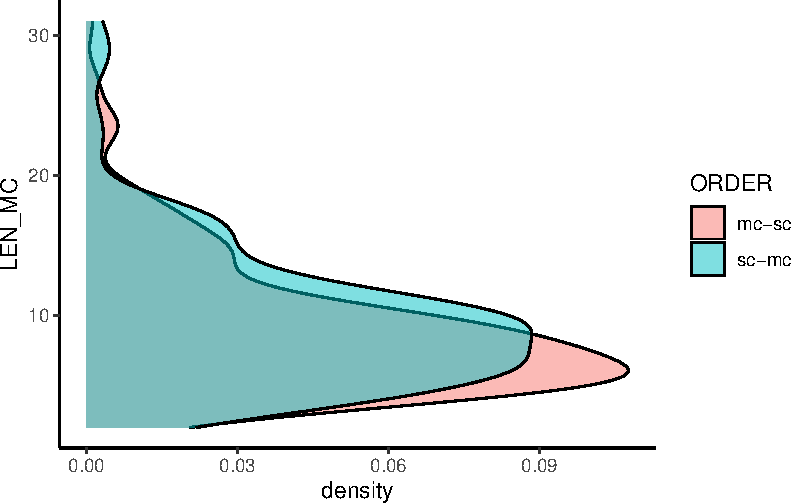
\includegraphics{Summary_statistics_files/figure-pdf/unnamed-chunk-24-1.pdf}

\section{Visualising mixed data}\label{visualising-mixed-data}

\subsection{A numerical and categorical
variable}\label{a-numerical-and-categorical-variable}

\begin{itemize}
\tightlist
\item
  Boxplot with \texttt{geom\_boxplot()}
\end{itemize}

\begin{Shaded}
\begin{Highlighting}[]
\FunctionTok{ggplot}\NormalTok{(cl.order, }\FunctionTok{aes}\NormalTok{(}\AttributeTok{x =}\NormalTok{ ORDER, }\AttributeTok{y =}\NormalTok{ LEN\_MC)) }\SpecialCharTok{+}
  \FunctionTok{geom\_boxplot}\NormalTok{()}
\end{Highlighting}
\end{Shaded}

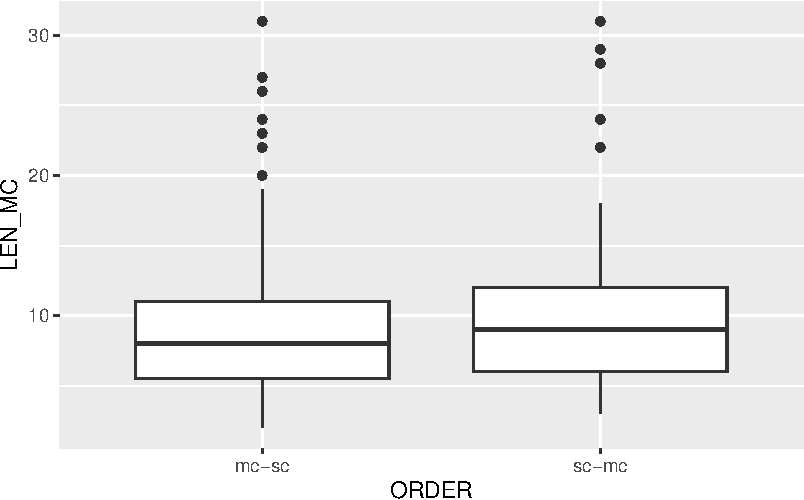
\includegraphics{Summary_statistics_files/figure-pdf/unnamed-chunk-25-1.pdf}

\begin{itemize}
\tightlist
\item
  Densitiy plot using the optional arguments \texttt{color} and/or
  \texttt{fill}
\end{itemize}

\begin{Shaded}
\begin{Highlighting}[]
\FunctionTok{ggplot}\NormalTok{(cl.order, }\FunctionTok{aes}\NormalTok{(}\AttributeTok{x =}\NormalTok{ LEN\_MC, }\AttributeTok{fill =}\NormalTok{ ORDER)) }\SpecialCharTok{+}
  \FunctionTok{geom\_density}\NormalTok{(}\AttributeTok{alpha =} \FloatTok{0.5}\NormalTok{)}
\end{Highlighting}
\end{Shaded}

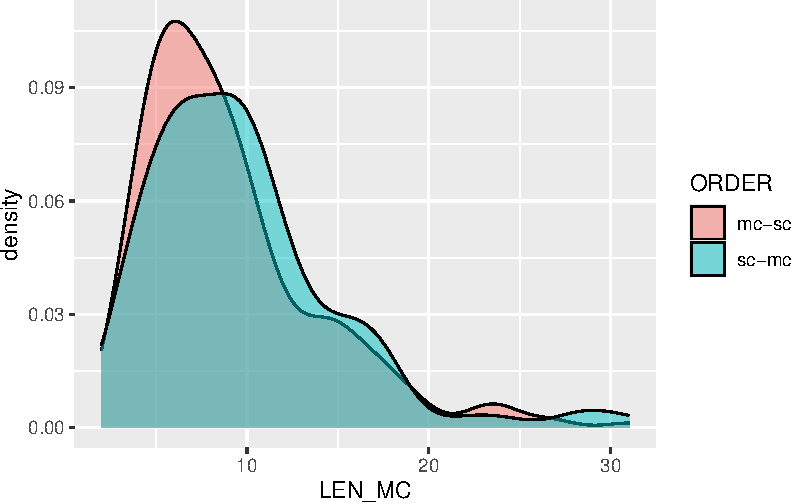
\includegraphics{Summary_statistics_files/figure-pdf/unnamed-chunk-26-1.pdf}

\begin{itemize}
\tightlist
\item
  A barplot with \texttt{geom\_col()}
\end{itemize}

\begin{Shaded}
\begin{Highlighting}[]
\FunctionTok{ggplot}\NormalTok{(cl.order, }\FunctionTok{aes}\NormalTok{(}\AttributeTok{x =}\NormalTok{ ORDER, }\AttributeTok{y =}\NormalTok{ LEN\_MC)) }\SpecialCharTok{+}
  \FunctionTok{geom\_col}\NormalTok{(}\FunctionTok{aes}\NormalTok{(}\AttributeTok{x =}\NormalTok{ ORDER, }\AttributeTok{y =}\NormalTok{ LEN\_MC))}
\end{Highlighting}
\end{Shaded}

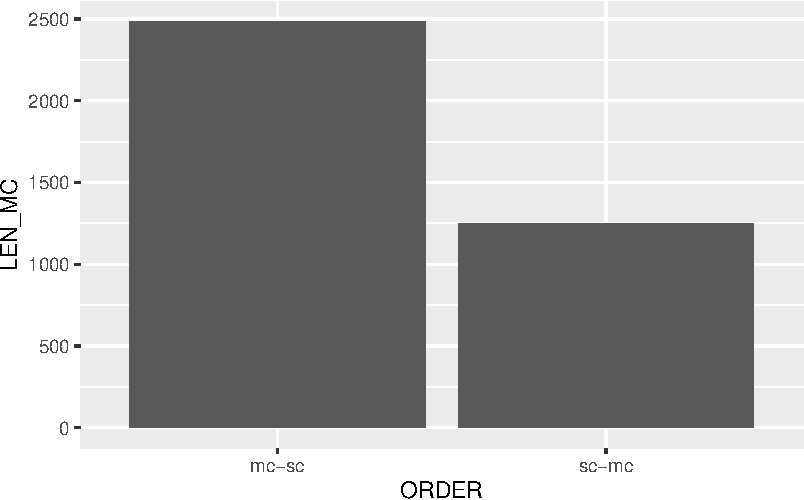
\includegraphics{Summary_statistics_files/figure-pdf/unnamed-chunk-27-1.pdf}

\subsection{Multivariate plots}\label{multivariate-plots}

\begin{itemize}
\tightlist
\item
  Advanced scatterplot with four variables: \texttt{LEN\_MC} (x),
  \texttt{LEN\_SC} (y), \texttt{ORDER} (colour) and \texttt{SUBORDTYPE}
  (shape)
\end{itemize}

\begin{Shaded}
\begin{Highlighting}[]
\CommentTok{\# 4 variables}
\FunctionTok{ggplot}\NormalTok{(cl.order, }\FunctionTok{aes}\NormalTok{(}\AttributeTok{x =}\NormalTok{ LEN\_MC, }\AttributeTok{y =}\NormalTok{ LEN\_SC)) }\SpecialCharTok{+}
  \FunctionTok{geom\_point}\NormalTok{(}\FunctionTok{aes}\NormalTok{(}\AttributeTok{color =}\NormalTok{ ORDER, }\AttributeTok{shape =}\NormalTok{ SUBORDTYPE))}
\end{Highlighting}
\end{Shaded}

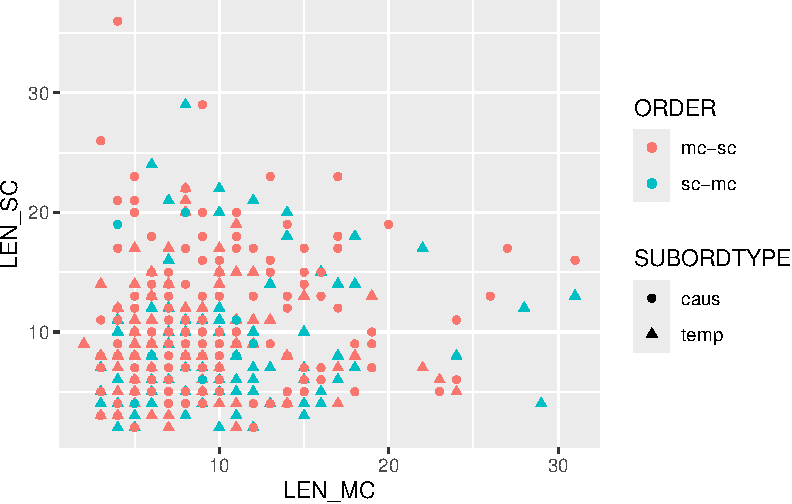
\includegraphics{Summary_statistics_files/figure-pdf/unnamed-chunk-28-1.pdf}

\begin{itemize}
\tightlist
\item
  Facets
\end{itemize}

\begin{Shaded}
\begin{Highlighting}[]
\CommentTok{\# 5 variables}
\FunctionTok{ggplot}\NormalTok{(cl.order, }\FunctionTok{aes}\NormalTok{(}\AttributeTok{x =}\NormalTok{ LEN\_MC, }\AttributeTok{y =}\NormalTok{ LEN\_SC)) }\SpecialCharTok{+}
  \FunctionTok{geom\_point}\NormalTok{(}\FunctionTok{aes}\NormalTok{(}\AttributeTok{color =}\NormalTok{ ORDER, }\AttributeTok{shape =}\NormalTok{ SUBORDTYPE)) }\SpecialCharTok{+}
  \FunctionTok{facet\_wrap}\NormalTok{(}\SpecialCharTok{\textasciitilde{}}\NormalTok{MORETHAN2CL)}
\end{Highlighting}
\end{Shaded}

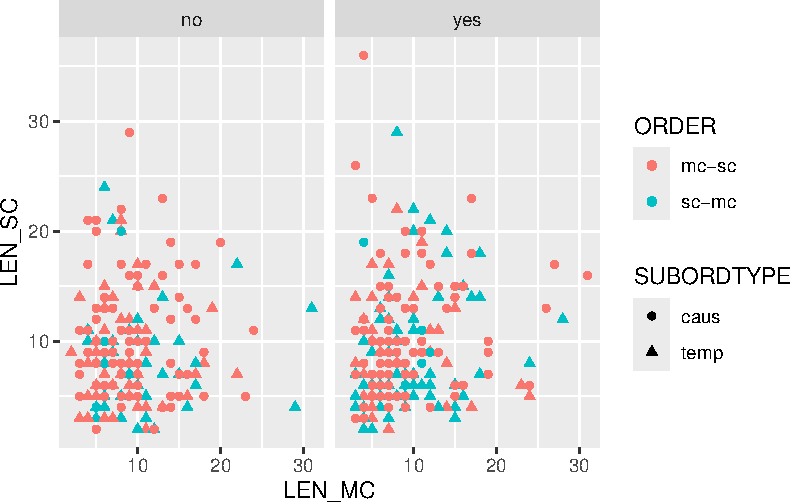
\includegraphics{Summary_statistics_files/figure-pdf/unnamed-chunk-29-1.pdf}

\chapter{Distributions}\label{distributions}

\section{The normal distribution}\label{the-normal-distribution}

A great number of numerical variables in the world follow the well-known
\textbf{normal} (or Gaussian) \textbf{distribution}, which includes test
scores, weight and height, among many others.

If a random variable \(X\) is normally distributed, it is determined by
the parameters \(\mu\) (the mean) and \(\sigma\) (the standard
deviation). Formally, we can summarise this using the notation

\[ X \sim N(\mu, \sigma^2).\] The \textbf{probability density function
(PDF)} of the normal distribution has a characteristic bell-shape. The
density values on the \(y\)-axis indicate the likelihood of encountering
a specific value of \(X\) (cf. Winter 2020: 56; Heumann, Schomaker, and
Shalabh 2022: 173-177).

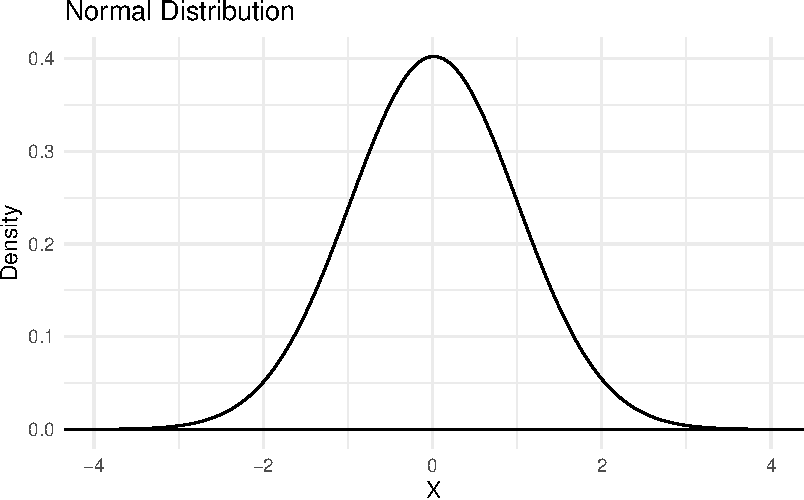
\includegraphics{Distributions_files/figure-pdf/unnamed-chunk-2-1.pdf}

\subsection{Bernoulli distribution}\label{bernoulli-distribution}

The \textbf{Bernoulli distribution} is a discrete probability
distribution for random variables which have only two possible outcomes:
``positive'' (often coded as 1) and ``negative'' (often coded as 0).
Examples of such variables include coin tosses (heads/tails), binary
response questions (yes/no), and defect status
(defective/non-defective).

If a random variable \(X\) follows a Bernoulli distribution, it is
determined by the parameter \(p\), which is the probability of the
positive case:

\[ X \sim Bernoulli(p).\] The \textbf{probability mass function (PMF)}
of the Bernoulli distribution is given by: \[
P(X = x) = 
\begin{cases} 
p & \text{if } x = 1 \\
1 - p & \text{if } x = 0 
\end{cases}
\]

where \(0 \leq p \leq 1\). This function shows the probability of \(X\)
taking on the value of 1 or 0 (cf. Heumann, Schomaker, and Shalabh 2022:
162-163).

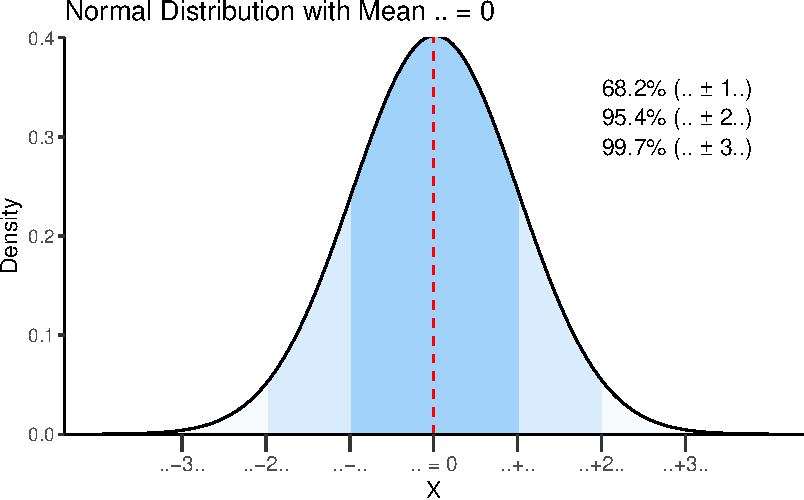
\includegraphics{Distributions_files/figure-pdf/unnamed-chunk-3-1.pdf}

\begin{tcolorbox}[enhanced jigsaw, toprule=.15mm, opacitybacktitle=0.6, coltitle=black, arc=.35mm, colback=white, title=\textcolor{quarto-callout-note-color}{\faInfo}\hspace{0.5em}{Extensions}, titlerule=0mm, toptitle=1mm, bottomtitle=1mm, breakable, rightrule=.15mm, opacityback=0, bottomrule=.15mm, leftrule=.75mm, colframe=quarto-callout-note-color-frame, left=2mm, colbacktitle=quarto-callout-note-color!10!white]

A Bernoulli experiment presupposes a single trial (e.g., tossing a coin
once). If we are interested in the distribution of a binary discrete
variable over \(n\) Bernoulli trials, we can describe it in terms of the
\textbf{binomial distribution} (Heumann, Schomaker, and Shalabh 2022:
163-166).

Categorical variables with more than 2 outcomes and \(n\) Bernoulli
trials can be modelled using the \textbf{multinomial distribution}
(Heumann, Schomaker, and Shalabh 2022: 167-169).

\end{tcolorbox}

\part{Inferential statistics}

\chapter{Hypothesis testing}\label{hypothesis-testing}

\section{Preparation}\label{preparation-5}

\begin{itemize}
\tightlist
\item
  Load packages:
\end{itemize}

\begin{Shaded}
\begin{Highlighting}[]
\FunctionTok{library}\NormalTok{(}\StringTok{"readxl"}\NormalTok{)}
\FunctionTok{library}\NormalTok{(}\StringTok{"tidyverse"}\NormalTok{)}
\end{Highlighting}
\end{Shaded}

\begin{itemize}
\tightlist
\item
  Load the data sets:
\end{itemize}

\begin{Shaded}
\begin{Highlighting}[]
\NormalTok{data }\OtherTok{\textless{}{-}} \FunctionTok{read\_xlsx}\NormalTok{(}\StringTok{"Paquot\_Larsson\_2020\_data.xlsx"}\NormalTok{)}

\NormalTok{data\_vowels }\OtherTok{\textless{}{-}} \FunctionTok{read.csv}\NormalTok{(}\StringTok{"Vowels\_Apache.csv"}\NormalTok{, }\AttributeTok{sep =} \StringTok{"}\SpecialCharTok{\textbackslash{}t}\StringTok{"}\NormalTok{)}
\end{Highlighting}
\end{Shaded}

\section{Hypothesis testing}\label{hypothesis-testing-1}

The first step is to define the \textbf{null hypothesis} \(H_0\) and the
\textbf{alternative hypothesis} \(H_1\) (or \(H_a\)).

Given two categorical variables \(X\) and \(Y\), we assume under \(H_0\)
that both variables are independent from each other. This hypothesis
describes the ``default state of the world'' (James et al. 2021: 555),
i.e., what we would usually expect to see. By contrast, the alternative
hypothesis \(H_1\) states that \(X\) and \(Y\) are \textbf{not}
independent, i.e., that \(H_0\) does not hold.

In this unit, we will consider two scenarios:

\begin{enumerate}
\def\labelenumi{\arabic{enumi}.}
\tightlist
\item
  We are interested in finding out whether English clause \texttt{ORDER}
  (`sc-mc' or `mc-sc') depends on the type of the subordinate clause
  (\texttt{SUBORDTYPE}), which can be either temporal (`temp') or causal
  (`caus').
\end{enumerate}

Our hypotheses are:

\begin{itemize}
\item
  \(H_0:\) The variables \texttt{ORDER} and \texttt{SUBORDTYPE} are
  independent.
\item
  \(H_1:\) The variables \texttt{ORDER} and \texttt{SUBORDTYPE} are
  \textbf{not} independent.
\end{itemize}

\begin{enumerate}
\def\labelenumi{\arabic{enumi}.}
\setcounter{enumi}{1}
\tightlist
\item
  As part of a phonetic study, we compare the base frequencies of the F1
  formants for male and female speakers of Apache. We forward the
  following hypotheses:
\end{enumerate}

\begin{itemize}
\item
  \(H_0:\) mean \texttt{F1\ frequency} of men \(=\) mean
  \texttt{F1\ frequency} of women.
\item
  \(H_1:\) mean \texttt{F1\ frequency} of men \(\ne\) mean
  \texttt{F1\ frequency} of women.
\end{itemize}

Based on our data, we can decide to either \textbf{accept} or
\textbf{reject} \(H_0\). Rejecting \(H_0\) can be viewed as evidence in
favour of \(H_1\) and thus marks a potential `discovery' in the data.
However, there is always a chance that we accept or reject the wrong
hypothesis; the four possible constellations are summarised in the table
below (cf. Heumann, Schomaker, and Shalabh 2022: 223):

\begin{longtable}[]{@{}
  >{\raggedright\arraybackslash}p{(\columnwidth - 4\tabcolsep) * \real{0.2030}}
  >{\raggedright\arraybackslash}p{(\columnwidth - 4\tabcolsep) * \real{0.3985}}
  >{\raggedright\arraybackslash}p{(\columnwidth - 4\tabcolsep) * \real{0.3985}}@{}}
\toprule\noalign{}
\begin{minipage}[b]{\linewidth}\raggedright
\end{minipage} & \begin{minipage}[b]{\linewidth}\raggedright
\(H_0\) is true
\end{minipage} & \begin{minipage}[b]{\linewidth}\raggedright
\(H_0\) is not true
\end{minipage} \\
\midrule\noalign{}
\endhead
\bottomrule\noalign{}
\endlastfoot
\(H_0\) \textbf{is not rejected} &
\(\color{green}{\text{Correct decision}}\) &
\(\color{red}{\text{Type II } (\beta)\text{-error}}\) \\
\(H_0\) \textbf{is rejected} &
\(\color{red}{\text{Type I } (\alpha)\text{-error}}\) &
\(\color{green}{\text{Correct decision}}\) \\
\end{longtable}

The probability of a Type I error, which refers to the rejection of
\(H_0\) although it is true, is called the \textbf{significance level}
\(\alpha\), which has a conventional value of \(0.05\) (i.e., a 5\%
chance of committing a Type I error).

\section{Constructing the critical
region}\label{constructing-the-critical-region}

An important question remains: How great should the difference be for us
to reject \(H_0\)? The \(p\)-value measures \textbf{the probability of
encountering a specific value of a test statistic} under the assumption
that \(H_0\) holds. For example, a \(p\)-value of \(0.02\) means that we
would see a particular \(\chi^2\)-score (or \(T\), \(F\) etc.) only 2\%
of the time if \(X\) and \(Y\) were unrelated (or if there was no
difference between \(\bar{x}\) and \(\bar{y}\), respectively). Since our
significance level \(\alpha\) is set to \(0.05\), we only reject the
null hypothesis if this probability is lower than 5\%.

We obtain \(p\)-values by consulting the probability density functions
of the underlying distributions:

\begin{itemize}
\tightlist
\item
  Probability density function for the \(\chi^2\)-distribution with
  \(df = 1\)
\end{itemize}

\begin{Shaded}
\begin{Highlighting}[]
\CommentTok{\# Generate random samples from a chi{-}squared distribution with 1 degree of freedom}
\NormalTok{x }\OtherTok{\textless{}{-}} \FunctionTok{rchisq}\NormalTok{(}\DecValTok{100000}\NormalTok{, }\AttributeTok{df =} \DecValTok{1}\NormalTok{)}

\CommentTok{\# Create histogram}
\FunctionTok{hist}\NormalTok{(x,}
     \AttributeTok{breaks =} \StringTok{"Scott"}\NormalTok{,}
     \AttributeTok{freq =} \ConstantTok{FALSE}\NormalTok{,}
     \AttributeTok{xlim =} \FunctionTok{c}\NormalTok{(}\DecValTok{0}\NormalTok{, }\DecValTok{20}\NormalTok{),}
     \AttributeTok{ylim =} \FunctionTok{c}\NormalTok{(}\DecValTok{0}\NormalTok{, }\FloatTok{0.2}\NormalTok{),}
     \AttributeTok{ylab =} \StringTok{"Probability density of observing a specific score"}\NormalTok{,}
     \AttributeTok{xlab =} \StringTok{"Chi{-}squared score"}\NormalTok{,}
     \AttributeTok{main =} \StringTok{"Histogram for a chi{-}squared distribution with 1 degree of freedom (df)"}\NormalTok{,}
     \AttributeTok{cex.main =} \FloatTok{0.9}\NormalTok{)}

\CommentTok{\# Overlay PDF}
\FunctionTok{curve}\NormalTok{(}\FunctionTok{dchisq}\NormalTok{(x, }\AttributeTok{df =} \DecValTok{1}\NormalTok{), }\AttributeTok{from =} \DecValTok{0}\NormalTok{, }\AttributeTok{to =} \DecValTok{150}\NormalTok{, }\AttributeTok{n =} \DecValTok{5000}\NormalTok{, }\AttributeTok{col =} \StringTok{"orange"}\NormalTok{, }\AttributeTok{lwd =} \DecValTok{2}\NormalTok{, }\AttributeTok{add =} \ConstantTok{TRUE}\NormalTok{)}
\end{Highlighting}
\end{Shaded}

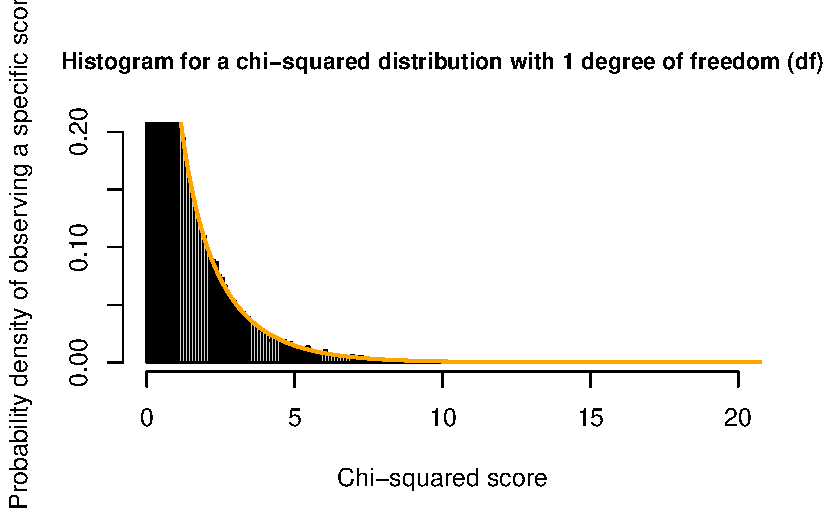
\includegraphics{Hypothesis_testing_files/figure-pdf/unnamed-chunk-4-1.pdf}

\begin{itemize}
\tightlist
\item
  Probability density function for the \(t\)-distribution with
  \(df = 112.19\)
\end{itemize}

\begin{Shaded}
\begin{Highlighting}[]
\CommentTok{\# Given t{-}statistic and degrees of freedom}
\NormalTok{t\_statistic }\OtherTok{\textless{}{-}} \FloatTok{2.4416}
\NormalTok{df }\OtherTok{\textless{}{-}} \FloatTok{112.19}

\CommentTok{\# Generate random samples from a t{-}distribution with the given degrees of freedom}
\NormalTok{x }\OtherTok{\textless{}{-}} \FunctionTok{rt}\NormalTok{(}\DecValTok{100000}\NormalTok{, }\AttributeTok{df =}\NormalTok{ df)}

\CommentTok{\# Create histogram}
\FunctionTok{hist}\NormalTok{(x,}
     \AttributeTok{breaks =} \StringTok{"Scott"}\NormalTok{,}
     \AttributeTok{freq =} \ConstantTok{FALSE}\NormalTok{,}
     \AttributeTok{xlim =} \FunctionTok{c}\NormalTok{(}\SpecialCharTok{{-}}\DecValTok{5}\NormalTok{, }\DecValTok{5}\NormalTok{),}
     \AttributeTok{ylim =} \FunctionTok{c}\NormalTok{(}\DecValTok{0}\NormalTok{, }\FloatTok{0.4}\NormalTok{),}
     \AttributeTok{ylab =} \StringTok{"Probability density of observing a specific score"}\NormalTok{,}
     \AttributeTok{xlab =} \StringTok{"t{-}score"}\NormalTok{,}
     \AttributeTok{main =} \StringTok{"Histogram for a t{-}distribution with 112.19 degrees of freedom"}\NormalTok{,}
     \AttributeTok{cex.main =} \FloatTok{0.9}\NormalTok{)}

\CommentTok{\# Overlay PDF}
\FunctionTok{curve}\NormalTok{(}\FunctionTok{dt}\NormalTok{(x, }\AttributeTok{df =}\NormalTok{ df), }\AttributeTok{from =} \SpecialCharTok{{-}}\DecValTok{5}\NormalTok{, }\AttributeTok{to =} \DecValTok{5}\NormalTok{, }\AttributeTok{n =} \DecValTok{5000}\NormalTok{, }\AttributeTok{col =} \StringTok{"orange"}\NormalTok{, }\AttributeTok{lwd =} \DecValTok{2}\NormalTok{, }\AttributeTok{add =} \ConstantTok{TRUE}\NormalTok{)}
\end{Highlighting}
\end{Shaded}

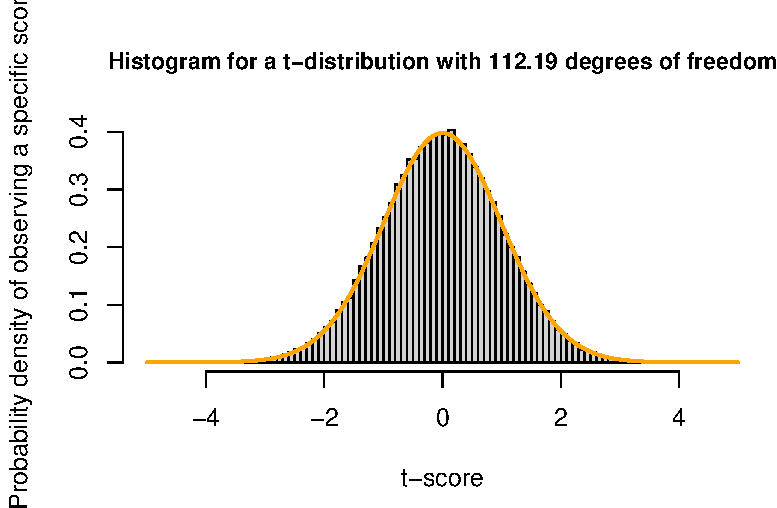
\includegraphics{Hypothesis_testing_files/figure-pdf/unnamed-chunk-5-1.pdf}

\chapter{Chi square test}\label{chi-square-test}

\section{Preparation}\label{preparation-6}

\begin{itemize}
\tightlist
\item
  Load packages:
\end{itemize}

\begin{Shaded}
\begin{Highlighting}[]
\FunctionTok{library}\NormalTok{(}\StringTok{"readxl"}\NormalTok{)}
\FunctionTok{library}\NormalTok{(}\StringTok{"tidyverse"}\NormalTok{)}
\end{Highlighting}
\end{Shaded}

\begin{itemize}
\tightlist
\item
  Load the data sets:
\end{itemize}

\begin{Shaded}
\begin{Highlighting}[]
\NormalTok{cl.order }\OtherTok{\textless{}{-}} \FunctionTok{read\_xlsx}\NormalTok{(}\StringTok{"Paquot\_Larsson\_2020\_data.xlsx"}\NormalTok{)}
\end{Highlighting}
\end{Shaded}

\section{Overview}\label{overview-1}

\begin{tcolorbox}[enhanced jigsaw, toprule=.15mm, opacitybacktitle=0.6, coltitle=black, arc=.35mm, colback=white, title=\textcolor{quarto-callout-note-color}{\faInfo}\hspace{0.5em}{This unit in a nutshell}, titlerule=0mm, toptitle=1mm, bottomtitle=1mm, breakable, rightrule=.15mm, opacityback=0, bottomrule=.15mm, leftrule=.75mm, colframe=quarto-callout-note-color-frame, left=2mm, colbacktitle=quarto-callout-note-color!10!white]

The chi-square test helps determine if there is a statistically
significant association between two categorical variables. It compares
observed frequencies (actual data) with expected frequencies (if the
null hypothesis were true). The greater the difference, the higher the
\(\chi^2\) score, providing evidence against \(H_0\)

\begin{itemize}
\tightlist
\item
  \(p\)-value: Indicates significance level.
\item
  \(\chi^2\) score: Shows the deviation between observed and expected
  frequencies.
\item
  Degrees of freedom: Affects the shape of the chi-square distribution.
\end{itemize}

If the \(p\)-value is below 0.05, we reject \(H_0\), indicating a
significant association between the variables.

Example:

\begin{Shaded}
\begin{Highlighting}[]
\CommentTok{\# Hypotheses:}
\CommentTok{\# H0: ORDER and SUBORDTYPE are independent.}
\CommentTok{\# H1: ORDER and SUBORDTYPE are not independent.}

\FunctionTok{chisq.test}\NormalTok{(cl.order}\SpecialCharTok{$}\NormalTok{ORDER, cl.order}\SpecialCharTok{$}\NormalTok{SUBORDTYPE)}
\end{Highlighting}
\end{Shaded}

\begin{verbatim}

    Pearson's Chi-squared test with Yates' continuity correction

data:  cl.order$ORDER and cl.order$SUBORDTYPE
X-squared = 104.24, df = 1, p-value < 2.2e-16
\end{verbatim}

\begin{Shaded}
\begin{Highlighting}[]
\CommentTok{\# We can reject H0 and accept H1.}
\end{Highlighting}
\end{Shaded}

\end{tcolorbox}

\section{\texorpdfstring{The
\(\chi^2\)-test}{The \textbackslash chi\^{}2-test}}\label{the-chi2-test}

Having clearly stated our hypotheses in the previous unit, the next step
is to compute a test statistic that indicates how strongly our data
conforms to \(H_0\). For instance, the Pearson \(\chi^2\) statistic is
commonly used for categorical variables.

It requires two types of values: the \textbf{observed frequencies}
\(n_{ij}\) in our data set and the \textbf{expected frequencies}
\(m_{ij}\), which we would expect to see if \(H_0\) were true. The
indices \(i\) and \(j\) uniquely identify the frequencies found in all
column-row combinations of a cross-table.

\begin{tcolorbox}[enhanced jigsaw, toprule=.15mm, opacitybacktitle=0.6, coltitle=black, arc=.35mm, colback=white, title=\textcolor{quarto-callout-note-color}{\faInfo}\hspace{0.5em}{Mathematical details: The structure of a contingency table}, titlerule=0mm, toptitle=1mm, bottomtitle=1mm, breakable, rightrule=.15mm, opacityback=0, bottomrule=.15mm, leftrule=.75mm, colframe=quarto-callout-note-color-frame, left=2mm, colbacktitle=quarto-callout-note-color!10!white]

The table below represents a generic contingency table where \(X\) and
\(Y\) are categorical variables. Each \(x_i\) represents a category of
\(X\) and each \(y_j\) represents a category of \(Y\). In the table,
each cell indicates the count of observation \(n_{ij}\) corresponding to
the \(i\)-th row and \(j\)-th column.

\begin{longtable}[]{@{}lllllll@{}}
\toprule\noalign{}
& & & \(Y\) & & & \\
\midrule\noalign{}
\endhead
\bottomrule\noalign{}
\endlastfoot
& & \(y_1\) & \(y_2\) & \ldots{} & \(y_J\) & \\
& \(x_1\) & \(n_{11}\) & \(n_{12}\) & \ldots{} & \(n_{1J}\) & \\
& \(x_2\) & \(n_{21}\) & \(n_{22}\) & \ldots{} & \(n_{2J}\) & \\
\(X\) & \ldots{} & \ldots{} & \ldots{} & \ldots{} & \ldots{} & \\
& \(x_I\) & \(n_{I1}\) & \(n_{I2}\) & \ldots{} & \(n_{3J}\) & \\
\end{longtable}

This is really just an abstraction of the cross-tables we've computed so
many times before.

\end{tcolorbox}

These are our observed frequencies \(n_{ij}\):

\begin{verbatim}
       
        caus temp
  mc-sc  184   91
  sc-mc   15  113
\end{verbatim}

The expected frequencies \(m_{ij}\) are calculated by

\[
m_{ij} = \frac{i\textrm{th row sum} \times j \textrm{th column sum}}{\textrm{number of observations}}.
\] T

he expected frequencies for our combination of variables is shown below.
In which cells can you see the greatest deviations between observed and
expected frequencies?

\begin{verbatim}
           caus      temp
mc-sc 135.79404 139.20596
sc-mc  63.20596  64.79404
\end{verbatim}

The \(\chi^2\)-test now offers a convenient way of quantifying the
differences between the two tables above. Given \(n\) observations and
\(k\) degrees of freedom (\(df\))\footnote{The degrees of freedom are
  calculated by
  \((\textrm{number of rows} -1) \times (\textrm{number of columns} - 1)\).},
the \(\chi^2\)-statistic measures how much the observed frequencies
\textbf{deviate} from the expected frequencies \textbf{for each cell} in
a contingency table (cf. Heumann, Schomaker, and Shalabh 2022: 249-251).

\begin{tcolorbox}[enhanced jigsaw, toprule=.15mm, opacitybacktitle=0.6, coltitle=black, arc=.35mm, colback=white, title=\textcolor{quarto-callout-note-color}{\faInfo}\hspace{0.5em}{Mathematical details: Formal definition of the chi-square test}, titlerule=0mm, toptitle=1mm, bottomtitle=1mm, breakable, rightrule=.15mm, opacityback=0, bottomrule=.15mm, leftrule=.75mm, colframe=quarto-callout-note-color-frame, left=2mm, colbacktitle=quarto-callout-note-color!10!white]

The joint deviations make up the final \(\chi^2\)-score, which is
defined as

\[
\chi^2 = \sum_{i=1}^{I}\sum_{i=j}^{J}{\frac{(n_{ij} - m_{ij})^2}{m_{ij}}}.
\]

\end{tcolorbox}

Note, however, that this test comes with certain statistical
assumptions. Violations of these assumptions decrease the validity of
the result and could, therefore, lead to wrong conclusions about
relationships in the data.

\begin{enumerate}
\def\labelenumi{\arabic{enumi}.}
\tightlist
\item
  All observations are independent of each other.
\item
  80\% of the expected frequencies are \(\geq\) 5.
\item
  All observed frequencies are \(\geq\) 1.
\end{enumerate}

In R, conducting this test is a simple one-liner:

\begin{Shaded}
\begin{Highlighting}[]
\NormalTok{freqs\_test }\OtherTok{\textless{}{-}} \FunctionTok{chisq.test}\NormalTok{(freqs)}

\FunctionTok{print}\NormalTok{(freqs\_test)}
\end{Highlighting}
\end{Shaded}

\begin{verbatim}

    Pearson's Chi-squared test with Yates' continuity correction

data:  freqs
X-squared = 104.24, df = 1, p-value < 2.2e-16
\end{verbatim}

The test object \texttt{freqs\_test} also stores the expected
frequencies, which we can also access. They appear to be all right:

\begin{Shaded}
\begin{Highlighting}[]
\CommentTok{\# Expected frequencies}
\NormalTok{freqs\_test}\SpecialCharTok{$}\NormalTok{expected}
\end{Highlighting}
\end{Shaded}

\begin{verbatim}
       
             caus      temp
  mc-sc 135.79404 139.20596
  sc-mc  63.20596  64.79404
\end{verbatim}

\begin{tcolorbox}[enhanced jigsaw, toprule=.15mm, opacitybacktitle=0.6, coltitle=black, arc=.35mm, colback=white, title=\textcolor{quarto-callout-important-color}{\faExclamation}\hspace{0.5em}{Important}, titlerule=0mm, toptitle=1mm, bottomtitle=1mm, breakable, rightrule=.15mm, opacityback=0, bottomrule=.15mm, leftrule=.75mm, colframe=quarto-callout-important-color-frame, left=2mm, colbacktitle=quarto-callout-important-color!10!white]

If the data does not meet the (expected) frequency requirements for the
\(\chi^2\)-test, the Fisher's Exact Test is a viable alternative (see
\texttt{?fisher.test()} for details).

\end{tcolorbox}

\section{Workflow in R}\label{workflow-in-r}

\subsection{\texorpdfstring{\(\chi^2\)-test}{\textbackslash chi\^{}2-test}}\label{chi2-test}

\subsubsection{Define hypotheses}\label{define-hypotheses}

\begin{itemize}
\item
  \(H_0:\) The variables \texttt{ORDER} and \texttt{SUBORDTYPE} are
  independent.
\item
  \(H_1:\) The variables \texttt{ORDER} and \texttt{SUBORDTYPE} are
  \textbf{not} independent.
\end{itemize}

\subsubsection{Running the test}\label{running-the-test}

\begin{Shaded}
\begin{Highlighting}[]
\CommentTok{\# Cross{-}tabulate the frequencies for the variables of interest}

\NormalTok{freqs }\OtherTok{\textless{}{-}} \FunctionTok{table}\NormalTok{(cl.order}\SpecialCharTok{$}\NormalTok{ORDER, cl.order}\SpecialCharTok{$}\NormalTok{SUBORDTYPE)}

\NormalTok{freqs }\DocumentationTok{\#\# Assumption met: all observed freqs =\textgreater{} 1}
\end{Highlighting}
\end{Shaded}

\begin{verbatim}
       
        caus temp
  mc-sc  184   91
  sc-mc   15  113
\end{verbatim}

\begin{Shaded}
\begin{Highlighting}[]
\CommentTok{\# Run a chis{-}quared test on the absolute frequencies and print the results}

\NormalTok{test }\OtherTok{\textless{}{-}} \FunctionTok{chisq.test}\NormalTok{(freqs, }\AttributeTok{correct =} \ConstantTok{FALSE}\NormalTok{)}

\CommentTok{\# Inspect expected frequencies}

\NormalTok{test}\SpecialCharTok{$}\NormalTok{expected }\CommentTok{\# Assumption met: all expected frequences =\textgreater{} 5}
\end{Highlighting}
\end{Shaded}

\begin{verbatim}
       
             caus      temp
  mc-sc 135.79404 139.20596
  sc-mc  63.20596  64.79404
\end{verbatim}

\begin{tcolorbox}[enhanced jigsaw, toprule=.15mm, opacitybacktitle=0.6, coltitle=black, arc=.35mm, colback=white, title=\textcolor{quarto-callout-tip-color}{\faLightbulb}\hspace{0.5em}{Advanced: Effect size}, titlerule=0mm, toptitle=1mm, bottomtitle=1mm, breakable, rightrule=.15mm, opacityback=0, bottomrule=.15mm, leftrule=.75mm, colframe=quarto-callout-tip-color-frame, left=2mm, colbacktitle=quarto-callout-tip-color!10!white]

The sample-size independent effect size measure \textbf{Cramer's
\emph{V}} (\(\phi\)) is defined as

\[V = \sqrt{\frac{\chi^2}{N \times df}}.\] The outcome varies between
\(0\) (= no correlation) and \(1\) (= perfect correlation); cf.~also
Gries (2013: 186).

\begin{Shaded}
\begin{Highlighting}[]
\CommentTok{\# Compute Cramer\textquotesingle{}s V}

\DocumentationTok{\#\# By hand:}

\CommentTok{\# Given chi{-}squared statistic}
\NormalTok{chi\_squared }\OtherTok{\textless{}{-}} \FunctionTok{unname}\NormalTok{(test}\SpecialCharTok{$}\NormalTok{statistic)}

\CommentTok{\# Total number of observations}
\NormalTok{total\_obs }\OtherTok{\textless{}{-}} \FunctionTok{sum}\NormalTok{(freqs)}

\FunctionTok{sqrt}\NormalTok{(chi\_squared }\SpecialCharTok{/}\NormalTok{ total\_obs }\SpecialCharTok{*}\NormalTok{ (}\FunctionTok{min}\NormalTok{(}\FunctionTok{dim}\NormalTok{(freqs)) }\SpecialCharTok{{-}} \DecValTok{1}\NormalTok{))}
\end{Highlighting}
\end{Shaded}

\begin{verbatim}
[1] 0.5139168
\end{verbatim}

\begin{Shaded}
\begin{Highlighting}[]
\DocumentationTok{\#\# Automatically:}
\FunctionTok{library}\NormalTok{(}\StringTok{"confintr"}\NormalTok{) }\CommentTok{\# Load library}

\FunctionTok{cramersv}\NormalTok{(test)}
\end{Highlighting}
\end{Shaded}

\begin{verbatim}
[1] 0.5139168
\end{verbatim}

\end{tcolorbox}

\subsubsection{Reporting the results}\label{reporting-the-results}

According to a \(\chi^2\)-test, there is a significant association
between clause \texttt{ORDER}and \texttt{SUBORDTYPE} at \(p < 0.001\)
(\(\chi^2 = 106.44, df = 1\)), thus justifying the rejection of \(H_0\).

\chapter{t-test}\label{t-test}

\begin{itemize}
\tightlist
\item
  Load packages:
\end{itemize}

\begin{Shaded}
\begin{Highlighting}[]
\FunctionTok{library}\NormalTok{(}\StringTok{"readxl"}\NormalTok{)}
\FunctionTok{library}\NormalTok{(}\StringTok{"tidyverse"}\NormalTok{)}
\end{Highlighting}
\end{Shaded}

\begin{Shaded}
\begin{Highlighting}[]
\NormalTok{data\_vowels }\OtherTok{\textless{}{-}} \FunctionTok{read.csv}\NormalTok{(}\StringTok{"Vowels\_Apache.csv"}\NormalTok{, }\AttributeTok{sep =} \StringTok{"}\SpecialCharTok{\textbackslash{}t}\StringTok{"}\NormalTok{)}
\end{Highlighting}
\end{Shaded}

\section{\texorpdfstring{The \(t\)-test}{The t-test}}\label{the-t-test}

Since the \(\chi^2\) measure exclusively works with categorical
variables, a separate test statistic is required if one of them is a
continuous variable. The \(t\) statistic is often used for research
questions involving differences between sample means. The way \(t\) is
calculated depends on the sources of \(X\) and \(Y\): Are they from the
same sample or from two (in-)dependent ones?

First, we consider two \textbf{independent samples} from a population:

\begin{itemize}
\item
  Sample \(X\) with the observations \(x_1, x_2, ..., {x_n}_1\), sample
  size \(n_1\), sample mean \(\bar{x}\) and sample variance \(s^2_x\).
\item
  Sample \(Y\) with the observations \(y_1, y_2, ..., {y_n}_2\), sample
  size \(n_2\), sample mean \(\bar{y}\) and sample variance \(s^2_y\).
\end{itemize}

\begin{tcolorbox}[enhanced jigsaw, toprule=.15mm, opacitybacktitle=0.6, coltitle=black, arc=.35mm, colback=white, title=\textcolor{quarto-callout-note-color}{\faInfo}\hspace{0.5em}{Definition of the \(t\)-test}, titlerule=0mm, toptitle=1mm, bottomtitle=1mm, breakable, rightrule=.15mm, opacityback=0, bottomrule=.15mm, leftrule=.75mm, colframe=quarto-callout-note-color-frame, left=2mm, colbacktitle=quarto-callout-note-color!10!white]

The \(t\)-statistic after Welch is given by:

\[
t(x, y) = \frac{|\bar{x} - \bar{y}|}{\sqrt{\frac{s^2_x}{n_1} + \frac{s^2_y}{n_2}}} 
\]

\begin{itemize}
\item
  If there is more than one observation for a given subject (e.g, before
  and after an experiment), the samples are called \textbf{dependent} or
  \textbf{paired}. The paired \(t\)-test assumes two continuous
  variables \(X\) and \(Y\).
\item
  In the paired test, the variable \(d\) denotes the difference between
  them, i.e., \(x - y\). The corresponding test statistic is obtained
  via
\end{itemize}

\[
t(x, y) = t(d) = \frac{\bar{d}}{s_d} \sqrt{n}.
\]

Note the difference \(\bar{d} = \frac{1}{n}\sum_{i=1}^n{d_i}\) and the
variance

\[
s^2_d = \frac{\sum_{i=1}^n({d_i} - \bar{d})^2}{n-1}.
\]

Traditionally, the \(t\)-test is based on the assumptions of \ldots{}

\begin{enumerate}
\def\labelenumi{\arabic{enumi}.}
\tightlist
\item
  \textbf{Normality} and
\item
  \textbf{Variance homogeneity} (i.e., equal sample variances). Note
  that this does not apply to the \(t\)-test after Welch, which can
  handle unequal variances.
\end{enumerate}

\end{tcolorbox}

\begin{tcolorbox}[enhanced jigsaw, toprule=.15mm, opacitybacktitle=0.6, coltitle=black, arc=.35mm, colback=white, title=\textcolor{quarto-callout-tip-color}{\faLightbulb}\hspace{0.5em}{Implementation in R: Manual vs.~automatic}, titlerule=0mm, toptitle=1mm, bottomtitle=1mm, breakable, rightrule=.15mm, opacityback=0, bottomrule=.15mm, leftrule=.75mm, colframe=quarto-callout-tip-color-frame, left=2mm, colbacktitle=quarto-callout-tip-color!10!white]

By hand:

\begin{Shaded}
\begin{Highlighting}[]
\CommentTok{\# Subset the data by sex}
\NormalTok{data\_m }\OtherTok{\textless{}{-}}\NormalTok{ data\_vowels[data\_vowels}\SpecialCharTok{$}\NormalTok{SEX }\SpecialCharTok{==} \StringTok{"M"}\NormalTok{, ]}
\NormalTok{data\_f }\OtherTok{\textless{}{-}}\NormalTok{ data\_vowels[data\_vowels}\SpecialCharTok{$}\NormalTok{SEX }\SpecialCharTok{==} \StringTok{"F"}\NormalTok{, ]}

\CommentTok{\# Compute sample means}
\NormalTok{mean\_m }\OtherTok{\textless{}{-}} \FunctionTok{mean}\NormalTok{(data\_m}\SpecialCharTok{$}\NormalTok{HZ\_F1)}
\NormalTok{mean\_f }\OtherTok{\textless{}{-}} \FunctionTok{mean}\NormalTok{(data\_f}\SpecialCharTok{$}\NormalTok{HZ\_F1)}

\CommentTok{\# Compute sample variances}
\NormalTok{var\_m }\OtherTok{\textless{}{-}} \FunctionTok{var}\NormalTok{(data\_m}\SpecialCharTok{$}\NormalTok{HZ\_F1)}
\NormalTok{var\_f }\OtherTok{\textless{}{-}} \FunctionTok{var}\NormalTok{(data\_f}\SpecialCharTok{$}\NormalTok{HZ\_F1)}

\CommentTok{\# Determine sample sizes}
\NormalTok{n\_m }\OtherTok{\textless{}{-}} \FunctionTok{length}\NormalTok{(data\_m}\SpecialCharTok{$}\NormalTok{HZ\_F1)}
\NormalTok{n\_f }\OtherTok{\textless{}{-}} \FunctionTok{length}\NormalTok{(data\_f}\SpecialCharTok{$}\NormalTok{HZ\_F1)}

\CommentTok{\# Compute t{-}statistic}
\NormalTok{t\_statistic }\OtherTok{\textless{}{-}} \FunctionTok{abs}\NormalTok{(mean\_m }\SpecialCharTok{{-}}\NormalTok{ mean\_f) }\SpecialCharTok{/} \FunctionTok{sqrt}\NormalTok{((var\_m }\SpecialCharTok{/}\NormalTok{ n\_m) }\SpecialCharTok{+}\NormalTok{ (var\_f }\SpecialCharTok{/}\NormalTok{ n\_f))}

\CommentTok{\# Compute degrees of freedom (simple version)}
\NormalTok{df }\OtherTok{\textless{}{-}}\NormalTok{ n\_m }\SpecialCharTok{+}\NormalTok{ n\_f }\SpecialCharTok{{-}} \DecValTok{2}

\CommentTok{\# Find the p{-}value using the cumulative distribution function (CDF) of the t{-}distribution}
\NormalTok{p\_value }\OtherTok{\textless{}{-}} \DecValTok{2} \SpecialCharTok{*} \FunctionTok{pt}\NormalTok{(}\SpecialCharTok{{-}}\NormalTok{t\_statistic, df)}
\end{Highlighting}
\end{Shaded}

Or, more concisely:

\begin{Shaded}
\begin{Highlighting}[]
\FunctionTok{t.test}\NormalTok{(data\_vowels}\SpecialCharTok{$}\NormalTok{HZ\_F1 }\SpecialCharTok{\textasciitilde{}}\NormalTok{ data\_vowels}\SpecialCharTok{$}\NormalTok{SEX, }\AttributeTok{paired =} \ConstantTok{FALSE}\NormalTok{) }\CommentTok{\# there is a significant difference!}
\end{Highlighting}
\end{Shaded}

\begin{verbatim}

    Welch Two Sample t-test

data:  data_vowels$HZ_F1 by data_vowels$SEX
t = 2.4416, df = 112.19, p-value = 0.01619
alternative hypothesis: true difference in means between group F and group M is not equal to 0
95 percent confidence interval:
  8.403651 80.758016
sample estimates:
mean in group F mean in group M 
       528.8548        484.2740 
\end{verbatim}

\end{tcolorbox}

\begin{tcolorbox}[enhanced jigsaw, toprule=.15mm, opacitybacktitle=0.6, coltitle=black, arc=.35mm, colback=white, title=\textcolor{quarto-callout-important-color}{\faExclamation}\hspace{0.5em}{Important}, titlerule=0mm, toptitle=1mm, bottomtitle=1mm, breakable, rightrule=.15mm, opacityback=0, bottomrule=.15mm, leftrule=.75mm, colframe=quarto-callout-important-color-frame, left=2mm, colbacktitle=quarto-callout-important-color!10!white]

If at least one assumption of the \(t\)-test has been violated, it is
important to use a non-parametric test such as the
\textbf{Wilcoxon-Mann-Whitney (WMW) U-Test} instead. In essence, this
test compares the probabilities of encountering a value \(x\) from
sample \(X\) that is greater than a value \(y\) from sample \(Y\). For
details, see \texttt{?wilcox.test()}.

\end{tcolorbox}

\section{Workflow in R}\label{workflow-in-r-1}

\subsection{Define hypotheses}\label{define-hypotheses-1}

\begin{itemize}
\item
  \(H_0:\) mean \texttt{F1\ frequency} of men \(=\) mean
  \texttt{F1\ frequency} of women.
\item
  \(H_1:\) mean \texttt{F1\ frequency} of men \(\ne\) mean
  \texttt{F1\ frequency} of women.
\end{itemize}

\subsection{Descriptive overview}\label{descriptive-overview}

We select the variables of interest and proceed calculate the mean
\texttt{F1\ frequencies} for each level of \texttt{SEX}, requiring a
grouped data frame.

\begin{Shaded}
\begin{Highlighting}[]
\CommentTok{\# Filter data so as to show only those observations that are relevant}

\NormalTok{data\_vowels }\SpecialCharTok{\%\textgreater{}\%} 
  \CommentTok{\# Filter columns}
  \FunctionTok{select}\NormalTok{(HZ\_F1, SEX) }\SpecialCharTok{\%\textgreater{}\%}
    \CommentTok{\# Define grouping variable}
    \FunctionTok{group\_by}\NormalTok{(SEX) }\SpecialCharTok{\%\textgreater{}\%} 
      \CommentTok{\# Compute mean and standard deviation for each sex}
      \FunctionTok{summarise}\NormalTok{(}\AttributeTok{mean =} \FunctionTok{mean}\NormalTok{(HZ\_F1),}
                \AttributeTok{sd =} \FunctionTok{sd}\NormalTok{(HZ\_F1)) }\OtherTok{{-}\textgreater{}}\NormalTok{ data\_vowels\_stats}

\NormalTok{knitr}\SpecialCharTok{::}\FunctionTok{kable}\NormalTok{(data\_vowels\_stats)}
\end{Highlighting}
\end{Shaded}

\begin{longtable}[]{@{}lrr@{}}
\toprule\noalign{}
SEX & mean & sd \\
\midrule\noalign{}
\endhead
\bottomrule\noalign{}
\endlastfoot
F & 528.8548 & 110.80099 \\
M & 484.2740 & 87.90112 \\
\end{longtable}

\begin{Shaded}
\begin{Highlighting}[]
\CommentTok{\# Plot distribution}

\DocumentationTok{\#\# Plot means}

\NormalTok{data\_vowels\_stats }\SpecialCharTok{\%\textgreater{}\%} 
  \FunctionTok{ggplot}\NormalTok{(}\FunctionTok{aes}\NormalTok{(}\AttributeTok{x =}\NormalTok{ SEX, }\AttributeTok{y =}\NormalTok{ mean)) }\SpecialCharTok{+}
    \FunctionTok{geom\_col}\NormalTok{() }\SpecialCharTok{+}
    \FunctionTok{geom\_errorbar}\NormalTok{(}\FunctionTok{aes}\NormalTok{(}\AttributeTok{x =}\NormalTok{ SEX,}
                    \AttributeTok{ymin =}\NormalTok{ mean}\SpecialCharTok{{-}}\NormalTok{sd,}
                    \AttributeTok{ymax =}\NormalTok{ mean}\SpecialCharTok{+}\NormalTok{sd), }\AttributeTok{width =}\NormalTok{ .}\DecValTok{2}\NormalTok{) }\SpecialCharTok{+}
    \FunctionTok{theme\_classic}\NormalTok{()}
\end{Highlighting}
\end{Shaded}

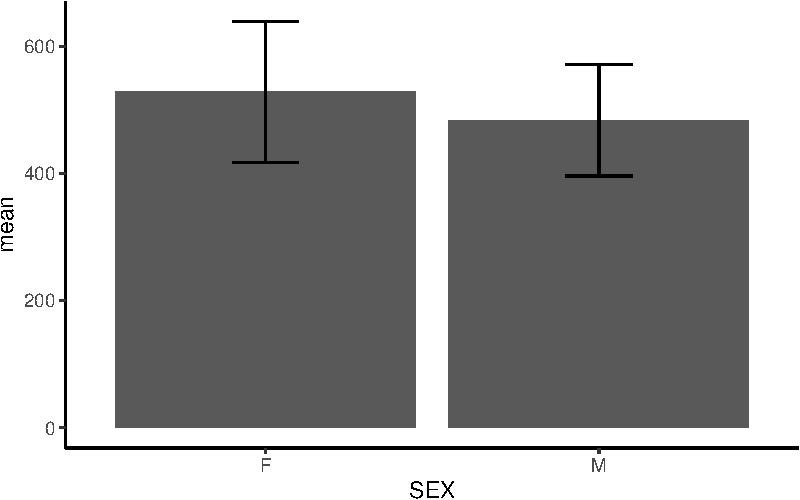
\includegraphics{t_test_files/figure-pdf/unnamed-chunk-7-1.pdf}

\begin{Shaded}
\begin{Highlighting}[]
\DocumentationTok{\#\# Plot quartiles}
\NormalTok{data\_vowels }\SpecialCharTok{\%\textgreater{}\%} 
  \FunctionTok{ggplot}\NormalTok{(}\FunctionTok{aes}\NormalTok{(}\AttributeTok{x =}\NormalTok{ SEX, }\AttributeTok{y =}\NormalTok{ HZ\_F1)) }\SpecialCharTok{+}
    \FunctionTok{geom\_boxplot}\NormalTok{() }\SpecialCharTok{+}
    \FunctionTok{theme\_classic}\NormalTok{()}
\end{Highlighting}
\end{Shaded}

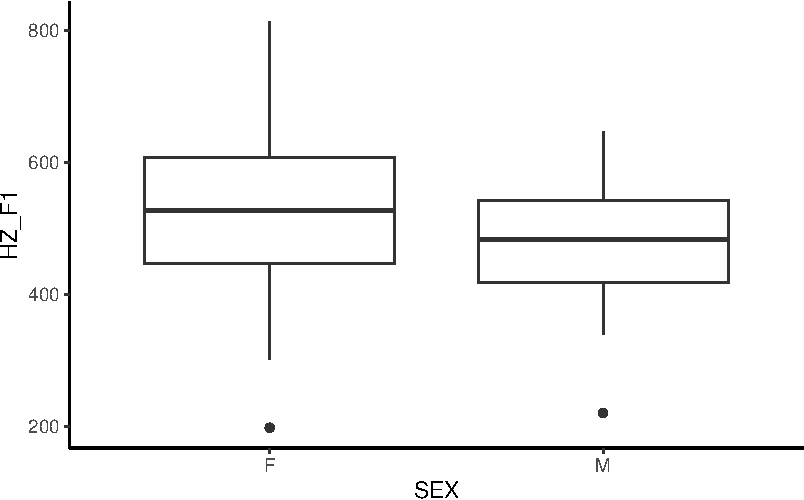
\includegraphics{t_test_files/figure-pdf/unnamed-chunk-7-2.pdf}

\subsection{\texorpdfstring{Check \(t\)-test
assumptions}{Check t-test assumptions}}\label{check-t-test-assumptions}

\begin{Shaded}
\begin{Highlighting}[]
\CommentTok{\# Normality}

\FunctionTok{shapiro.test}\NormalTok{(data\_vowels}\SpecialCharTok{$}\NormalTok{HZ\_F1) }\CommentTok{\# H0: data points follow the normal distribution}
\end{Highlighting}
\end{Shaded}

\begin{verbatim}

    Shapiro-Wilk normality test

data:  data_vowels$HZ_F1
W = 0.98996, p-value = 0.5311
\end{verbatim}

\begin{Shaded}
\begin{Highlighting}[]
\CommentTok{\# Check histogram}

\FunctionTok{ggplot}\NormalTok{(data\_vowels, }\FunctionTok{aes}\NormalTok{(}\AttributeTok{x =}\NormalTok{ HZ\_F1)) }\SpecialCharTok{+}
  \FunctionTok{geom\_histogram}\NormalTok{(}\AttributeTok{bins =} \DecValTok{30}\NormalTok{) }\SpecialCharTok{+}
  \FunctionTok{theme\_classic}\NormalTok{()}
\end{Highlighting}
\end{Shaded}

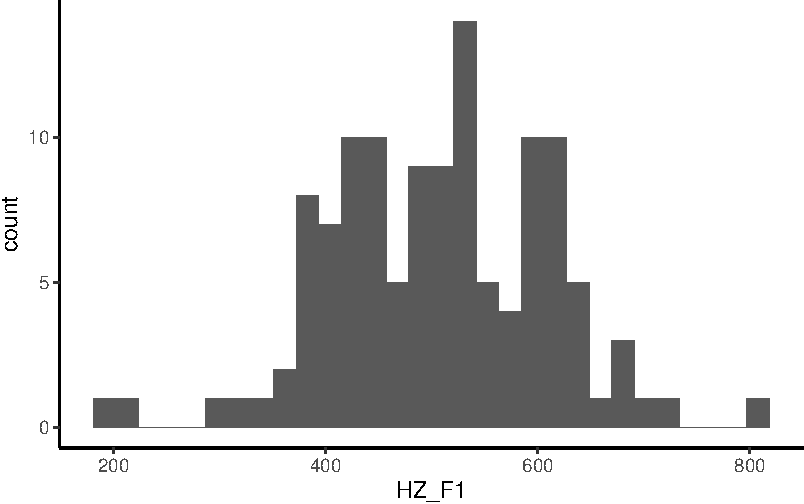
\includegraphics{t_test_files/figure-pdf/unnamed-chunk-8-1.pdf}

\begin{Shaded}
\begin{Highlighting}[]
\CommentTok{\# Variance homogeneity}

\FunctionTok{var.test}\NormalTok{(data\_vowels}\SpecialCharTok{$}\NormalTok{HZ\_F1 }\SpecialCharTok{\textasciitilde{}}\NormalTok{ data\_vowels}\SpecialCharTok{$}\NormalTok{SEX) }\CommentTok{\# H0: variances are not too different from each other}
\end{Highlighting}
\end{Shaded}

\begin{verbatim}

    F test to compare two variances

data:  data_vowels$HZ_F1 by data_vowels$SEX
F = 1.5889, num df = 59, denom df = 59, p-value = 0.07789
alternative hypothesis: true ratio of variances is not equal to 1
95 percent confidence interval:
 0.949093 2.660040
sample estimates:
ratio of variances 
          1.588907 
\end{verbatim}

\subsection{Running the test}\label{running-the-test-1}

\begin{Shaded}
\begin{Highlighting}[]
\CommentTok{\# t{-}test for two independent samples }

\FunctionTok{t.test}\NormalTok{(data\_vowels}\SpecialCharTok{$}\NormalTok{HZ\_F1 }\SpecialCharTok{\textasciitilde{}}\NormalTok{ data\_vowels}\SpecialCharTok{$}\NormalTok{SEX, }\AttributeTok{paired =} \ConstantTok{FALSE}\NormalTok{) }\CommentTok{\# there is a significant difference!}
\end{Highlighting}
\end{Shaded}

\begin{verbatim}

    Welch Two Sample t-test

data:  data_vowels$HZ_F1 by data_vowels$SEX
t = 2.4416, df = 112.19, p-value = 0.01619
alternative hypothesis: true difference in means between group F and group M is not equal to 0
95 percent confidence interval:
  8.403651 80.758016
sample estimates:
mean in group F mean in group M 
       528.8548        484.2740 
\end{verbatim}

\subsection{Optional: Effect size}\label{optional-effect-size}

\textbf{Cohen's} \textbf{\emph{d}} is a possible effect size measure for
continuous data and is obtained by dividing the difference of both
sample means by the pooled standard deviation:

\[\frac{\bar{x} - \bar{y}}{\sqrt{\frac{{(n_1 - 1)s_x^2 + (n_2 - 1)s_y^2}}{{n_1 + n_2 - 2}}}}.\]

\begin{Shaded}
\begin{Highlighting}[]
\FunctionTok{library}\NormalTok{(}\StringTok{"effsize"}\NormalTok{)}

\CommentTok{\# By hand:}
\DocumentationTok{\#\# Compute pooled standard deviation sp}
\NormalTok{sp }\OtherTok{\textless{}{-}} \FunctionTok{sqrt}\NormalTok{(((n\_m }\SpecialCharTok{{-}} \DecValTok{1}\NormalTok{) }\SpecialCharTok{*}\NormalTok{ var\_m }\SpecialCharTok{+}\NormalTok{ (n\_f }\SpecialCharTok{{-}} \DecValTok{1}\NormalTok{) }\SpecialCharTok{*}\NormalTok{ var\_f) }\SpecialCharTok{/}\NormalTok{ (n\_m }\SpecialCharTok{+}\NormalTok{ n\_f }\SpecialCharTok{{-}} \DecValTok{2}\NormalTok{))}

\DocumentationTok{\#\# Compute Cohen\textquotesingle{}s d}
\NormalTok{d }\OtherTok{\textless{}{-}} \FunctionTok{abs}\NormalTok{(mean\_m }\SpecialCharTok{{-}}\NormalTok{ mean\_f) }\SpecialCharTok{/}\NormalTok{ sp}

\CommentTok{\# Automatically:}
\FunctionTok{cohen.d}\NormalTok{(data\_vowels}\SpecialCharTok{$}\NormalTok{HZ\_F1, data\_vowels}\SpecialCharTok{$}\NormalTok{SEX) }\CommentTok{\# see also ?cohen.d for more details}
\end{Highlighting}
\end{Shaded}

\begin{verbatim}

Cohen's d

d estimate: 0.4457697 (small)
95 percent confidence interval:
     lower      upper 
0.07976048 0.81177897 
\end{verbatim}

\subsection{Reporting the results}\label{reporting-the-results-1}

According to a two-sample \(t\)-test, there is a significant difference
between the mean \texttt{F1\ frequencies} of male and female speakers of
Apache (\(t = 2.44\), \(df = 112.19\), \(p < 0.05\)). Therefore, \(H_0\)
will be rejected.

\part{Machine learning}

\chapter{Linear regression}\label{linear-regression}

\section{Recommended reading}\label{recommended-reading-4}

\begin{quote}
The following introduction is based on Heumann et al. (2022: Chapter
11), James et al. (2021: Chapter 3), Levshina (2015: Chapter 7) and
Winter (2020: Chapter 4).
\end{quote}

\section{Preparation}\label{preparation-7}

\begin{Shaded}
\begin{Highlighting}[]
\CommentTok{\# Load libraries}

\FunctionTok{library}\NormalTok{(}\StringTok{"readxl"}\NormalTok{)}
\FunctionTok{library}\NormalTok{(}\StringTok{"writexl"}\NormalTok{)}
\FunctionTok{library}\NormalTok{(}\StringTok{"tidyverse"}\NormalTok{)}

\CommentTok{\# Load file}
\NormalTok{ELP }\OtherTok{\textless{}{-}} \FunctionTok{read\_xlsx}\NormalTok{(}\StringTok{"ELP.xlsx"}\NormalTok{)}

\CommentTok{\# Inspect file structure}
\FunctionTok{str}\NormalTok{(ELP)}
\end{Highlighting}
\end{Shaded}

\section{Introduction}\label{introduction}

Consider the distribution of the continuous variable \texttt{RT}
(reaction times) from the \texttt{ELP} (English Lexicon Project)
dataset. We will \(log\)-transform the reaction times to even out the
differences between extremely high and extremely low frequency counts
(cf. Winter 2020: 90-94).

\subsection{Log-transformed}

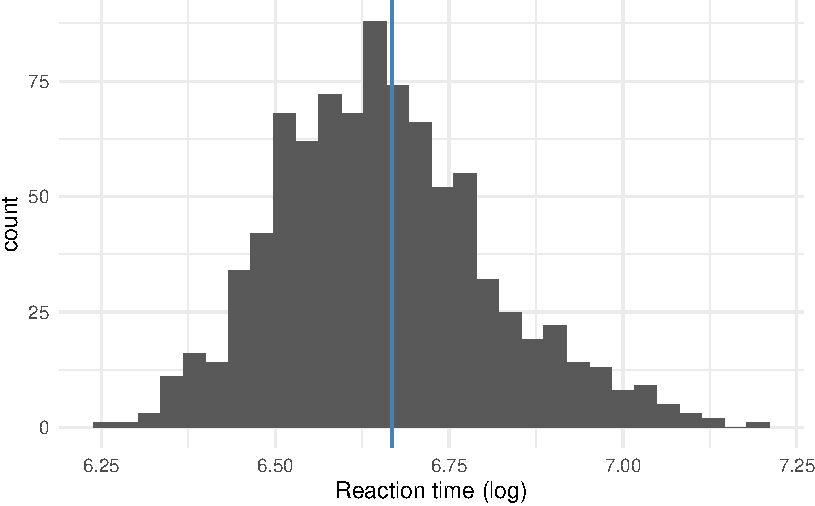
\includegraphics{Linear_regression_files/figure-pdf/unnamed-chunk-3-1.pdf}

\subsection{Default}

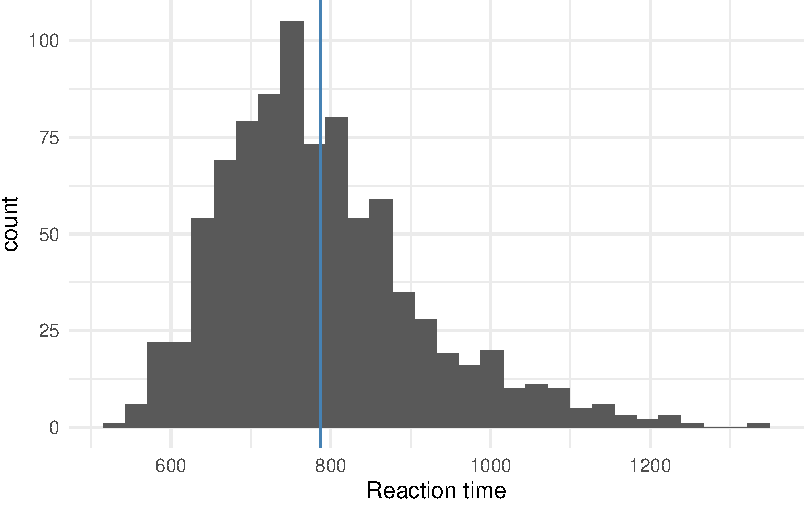
\includegraphics{Linear_regression_files/figure-pdf/unnamed-chunk-4-1.pdf}

We are investigating the relationship between reaction times \texttt{RT}
and the frequency \texttt{Freq} of a lexical stimulus.

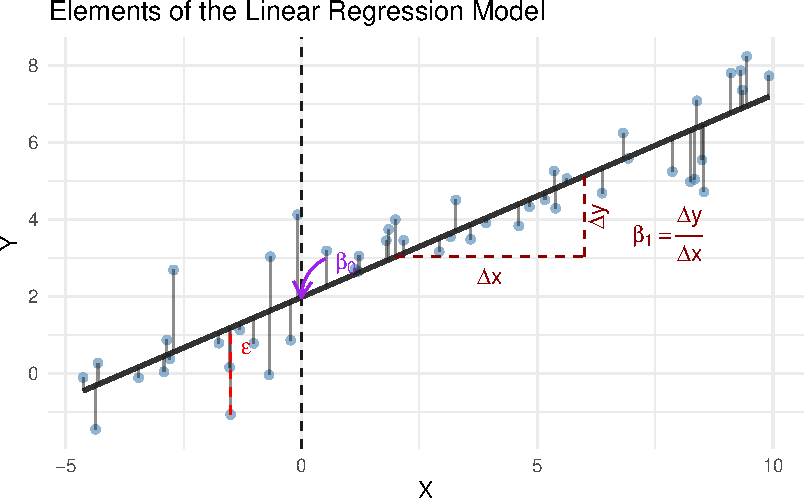
\includegraphics{Linear_regression_files/figure-pdf/unnamed-chunk-5-1.pdf}

\textbf{Some open questions}:

\begin{itemize}
\item
  Can word frequency help us explain variation in reaction times?
\item
  If it can, then how could we characterise the effect of word
  frequency? In other words, does it increase or decrease reaction
  times?
\item
  What reaction times should we expect for new observations?
\end{itemize}

\subsection{Building a statistical
model}\label{building-a-statistical-model}

Here \texttt{RT} is a \emph{response} or \emph{target} that we wish to
explain. We generically refer to the response as \(Y\).

\texttt{Freq} is a \emph{feature}, \emph{input}, or \emph{predictor},
which we name \(X\).

We can thus summarise our preliminary and fairly general statistical
model as

\[ Y = f(X) + \epsilon. \]While the term \(f(X)\) denotes the
contribution of \(X\) to the explanation of \(Y\), \(\epsilon\)
describes the errors of the model.

\section{Linear Regression}\label{linear-regression-1}

Linear regression is a simple approach to supervised machine learning
where the response variable is known. It assumes that the dependence of
\(Y\) on \(X\) is \textbf{linear}. This approach is suitable for
\textbf{numerical response variables}. The predictors, however, can be
either numerical or discrete/categorical. Although it may seem overly
simplistic, linear regression is \textbf{extremely useful} both
conceptually and practically.

\subsection{\texorpdfstring{Model with a single predictor
\(X\)}{Model with a single predictor X}}\label{model-with-a-single-predictor-x}

A linear model of our data would have the form

\[ Y = \beta_0 + \beta_1X + \epsilon \]

or, in more concrete terms,

\[ \text{Reaction time} = \beta_0 + \beta_1\text{Frequency} + \text{Model Error,} \]

where \(\beta_0\) and \(\beta_1\) are two unknown constants that
represent the \textbf{intercept} and \textbf{slope} of the regression
line, respectively. Together they are referred to as the model
\textbf{coefficients} (or parameters), and \(\epsilon\) is the error
term. The fact that assumptions are made about the form of the model
renders it a \textbf{parametric model}.

Given the existing data on \(X\) and \(Y\), which is also known as the
training data, we \textbf{estimate} the model coefficients \(\beta_0\)
and \(\beta_1\). While we use the training data to estimate these
coefficients, we cannot know the true values of the coefficients, i.e.,
the exact true relationship between the variables. Their tentative
nature is indicated by the \textbf{hat} symbol \^{} above them:
\(\hat{\beta_0}\) and \(\hat{\beta_1}\).

\begin{tcolorbox}[enhanced jigsaw, toprule=.15mm, opacitybacktitle=0.6, coltitle=black, arc=.35mm, colback=white, title=\textcolor{quarto-callout-tip-color}{\faLightbulb}\hspace{0.5em}{How are the coefficients estimated?}, titlerule=0mm, toptitle=1mm, bottomtitle=1mm, breakable, rightrule=.15mm, opacityback=0, bottomrule=.15mm, leftrule=.75mm, colframe=quarto-callout-tip-color-frame, left=2mm, colbacktitle=quarto-callout-tip-color!10!white]

The most common way of estimating parameters for linear models is the
\textbf{Least Squares} approach. In essence, the parameters are chosen
such that the residual sum of squares, i.e., the sum of the differences
between observed and predicted values, is as low as possible. More
formally, the estimated slope then corresponds to

\[ \hat{\beta}_1 = \frac{\sum_{i=1}^n(x_i - \bar{x})(y_i- \bar{y})}{\sum_{i=1}(x_i- \bar{x})^2}.\]

Now we can obtain the intercept:

\[
\hat{\beta_0}= \bar{y}- \hat{\beta}_1\bar{x}
\]

\end{tcolorbox}

We can then predict future sales using the formula

\[
\hat{y} = \hat{\beta}_0 + \hat{\beta}_1x,
\]

where \(\hat{y}\) indicates a prediction of \(Y\) on the basis of the
predictor values \(X = x\).

In R, we can fit a linear model with the \texttt{lm()} function.

\begin{Shaded}
\begin{Highlighting}[]
\CommentTok{\# Fit linear model}

\NormalTok{rt.lm1 }\OtherTok{=} \FunctionTok{lm}\NormalTok{(}\FunctionTok{log}\NormalTok{(RT) }\SpecialCharTok{\textasciitilde{}} \FunctionTok{log}\NormalTok{(Freq), }\AttributeTok{data =}\NormalTok{ ELP)}

\CommentTok{\# View model data}

\FunctionTok{summary}\NormalTok{(rt.lm1)}
\end{Highlighting}
\end{Shaded}

\begin{verbatim}

Call:
lm(formula = log(RT) ~ log(Freq), data = ELP)

Residuals:
     Min       1Q   Median       3Q      Max 
-0.29765 -0.08203 -0.01205  0.07298  0.43407 

Coefficients:
             Estimate Std. Error t value Pr(>|t|)    
(Intercept)  6.633361   0.004286 1547.82   <2e-16 ***
log(Freq)   -0.048602   0.002201  -22.08   <2e-16 ***
---
Signif. codes:  0 '***' 0.001 '**' 0.01 '*' 0.05 '.' 0.1 ' ' 1

Residual standard error: 0.1235 on 878 degrees of freedom
Multiple R-squared:  0.357, Adjusted R-squared:  0.3563 
F-statistic: 487.5 on 1 and 878 DF,  p-value: < 2.2e-16
\end{verbatim}

The model statistics comprise the following elements:

\begin{tcolorbox}[enhanced jigsaw, toprule=.15mm, opacitybacktitle=0.6, coltitle=black, arc=.35mm, colback=white, title=\textcolor{quarto-callout-tip-color}{\faLightbulb}\hspace{0.5em}{Call}, titlerule=0mm, toptitle=1mm, bottomtitle=1mm, breakable, rightrule=.15mm, opacityback=0, bottomrule=.15mm, leftrule=.75mm, colframe=quarto-callout-tip-color-frame, left=2mm, colbacktitle=quarto-callout-tip-color!10!white]

i.e., the model formula.

\end{tcolorbox}

\begin{tcolorbox}[enhanced jigsaw, toprule=.15mm, opacitybacktitle=0.6, coltitle=black, arc=.35mm, colback=white, title=\textcolor{quarto-callout-tip-color}{\faLightbulb}\hspace{0.5em}{Residuals}, titlerule=0mm, toptitle=1mm, bottomtitle=1mm, breakable, rightrule=.15mm, opacityback=0, bottomrule=.15mm, leftrule=.75mm, colframe=quarto-callout-tip-color-frame, left=2mm, colbacktitle=quarto-callout-tip-color!10!white]

These indicate the difference between the observed values in the data
set and the values predicted by the model (= the fitted values). These
correspond to the error term \(\epsilon\). The lower the residuals, the
better the model describes the data.

\begin{Shaded}
\begin{Highlighting}[]
\CommentTok{\# Show fitted values (= predictions) for the first six observations}

\FunctionTok{head}\NormalTok{(rt.lm1}\SpecialCharTok{$}\NormalTok{fitted.values)}
\end{Highlighting}
\end{Shaded}

\begin{verbatim}
       1        2        3        4        5        6 
6.635345 6.563152 6.789806 6.613980 6.630529 6.574894 
\end{verbatim}

\begin{Shaded}
\begin{Highlighting}[]
\CommentTok{\# Show deviation of the fitted values from the observed values}

\FunctionTok{head}\NormalTok{(rt.lm1}\SpecialCharTok{$}\NormalTok{residuals)}
\end{Highlighting}
\end{Shaded}

\begin{verbatim}
          1           2           3           4           5           6 
 0.03778825 -0.02277165  0.07759556  0.03387713  0.15222949 -0.10432670 
\end{verbatim}

\end{tcolorbox}

\begin{tcolorbox}[enhanced jigsaw, toprule=.15mm, opacitybacktitle=0.6, coltitle=black, arc=.35mm, colback=white, title=\textcolor{quarto-callout-tip-color}{\faLightbulb}\hspace{0.5em}{Coefficients}, titlerule=0mm, toptitle=1mm, bottomtitle=1mm, breakable, rightrule=.15mm, opacityback=0, bottomrule=.15mm, leftrule=.75mm, colframe=quarto-callout-tip-color-frame, left=2mm, colbacktitle=quarto-callout-tip-color!10!white]

The regression coefficients correspond to \(\hat{\beta}_0\)
(``Intercept'') and \(\hat{\beta}_1\) (``log(Freq)''), respectively. The
model shows that for a one-unit increase in log-frequency the
log-reaction time decreases by approx. -0.05.

\begin{Shaded}
\begin{Highlighting}[]
\CommentTok{\# Convert coefficients to a tibble }

\FunctionTok{library}\NormalTok{(}\StringTok{"broom"}\NormalTok{)}

\NormalTok{tidy\_model }\OtherTok{\textless{}{-}} \FunctionTok{tidy}\NormalTok{(rt.lm1)}

\NormalTok{tidy\_model}
\end{Highlighting}
\end{Shaded}

\begin{verbatim}
# A tibble: 2 x 5
  term        estimate std.error statistic  p.value
  <chr>          <dbl>     <dbl>     <dbl>    <dbl>
1 (Intercept)   6.63     0.00429    1548.  0       
2 log(Freq)    -0.0486   0.00220     -22.1 2.88e-86
\end{verbatim}

\end{tcolorbox}

\begin{tcolorbox}[enhanced jigsaw, toprule=.15mm, opacitybacktitle=0.6, coltitle=black, arc=.35mm, colback=white, title=\textcolor{quarto-callout-tip-color}{\faLightbulb}\hspace{0.5em}{\(p\)-values and \(t\)-statistic}, titlerule=0mm, toptitle=1mm, bottomtitle=1mm, breakable, rightrule=.15mm, opacityback=0, bottomrule=.15mm, leftrule=.75mm, colframe=quarto-callout-tip-color-frame, left=2mm, colbacktitle=quarto-callout-tip-color!10!white]

\(p\)\textbf{-values and} \(t\)\textbf{-statistic}: Given the null
hypothesis \(H_0\) that there is no correlation between \texttt{log(RT)}
and \texttt{log(Freq)} (i.e., \(H_0: \beta_1 = 0\)), a \(p\)-value lower
than 0.05 indicates that \(\beta_1\) considerably deviates from 0, thus
providing evidence for the alternative hypothesis
\(H_1: \beta_1 \ne 0\). Since \(p < 0.001\), we can reject \(H_0\).

\begin{verbatim}
The $p$-value itself crucially depends on the
$t$-statistic[^linear_regression-1], which measures "the number of
standard deviations that $\hat{\beta_1}$ is away from 0"
[@james_introduction_2021: 67] . The standard error (SE) reflects
how much an estimated coefficient differs on average from the true
values of $\beta_0$ and $\beta_1$. They can be used to compute the
95% confidence interval
$[\hat{\beta}_1 - 2 \cdot SE(\hat{β}_1), \hat{\beta}_1 + 2 \cdot SE(\hat{β}_1)]$;
the true estimate of the parameter $\beta_1$ lies within the
specified range 95% of the time.
\end{verbatim}

\begin{Shaded}
\begin{Highlighting}[]
\CommentTok{\# Compute confidence intervals for intercept and log(Freq)}

\NormalTok{tidy\_model\_ci }\OtherTok{\textless{}{-}} \FunctionTok{tidy}\NormalTok{(rt.lm1, }\AttributeTok{conf.int =} \ConstantTok{TRUE}\NormalTok{)}

\NormalTok{tidy\_model\_ci}
\end{Highlighting}
\end{Shaded}

\begin{verbatim}
# A tibble: 2 x 7
  term        estimate std.error statistic  p.value conf.low conf.high
  <chr>          <dbl>     <dbl>     <dbl>    <dbl>    <dbl>     <dbl>
1 (Intercept)   6.63     0.00429    1548.  0          6.62      6.64  
2 log(Freq)    -0.0486   0.00220     -22.1 2.88e-86  -0.0529   -0.0443
\end{verbatim}

The estimated parameter for \texttt{log(Freq)}, which is -0.049, thus
has the 95\% confidence interval {[}-0.053, -0.044{]}.

\end{tcolorbox}

\begin{tcolorbox}[enhanced jigsaw, toprule=.15mm, opacitybacktitle=0.6, coltitle=black, arc=.35mm, colback=white, title=\textcolor{quarto-callout-tip-color}{\faLightbulb}\hspace{0.5em}{\textbf{Residual standard error} (RSE)}, titlerule=0mm, toptitle=1mm, bottomtitle=1mm, breakable, rightrule=.15mm, opacityback=0, bottomrule=.15mm, leftrule=.75mm, colframe=quarto-callout-tip-color-frame, left=2mm, colbacktitle=quarto-callout-tip-color!10!white]

This is an estimation of the average deviation of the predictions from
the observed values.

\[RSE = \sqrt{\frac{1}{n-2}\sum_{i=1}^n (y_i - \hat{y_i}})^2\]

\end{tcolorbox}

\begin{tcolorbox}[enhanced jigsaw, toprule=.15mm, opacitybacktitle=0.6, coltitle=black, arc=.35mm, colback=white, title=\textcolor{quarto-callout-tip-color}{\faLightbulb}\hspace{0.5em}{\(R^2\)}, titlerule=0mm, toptitle=1mm, bottomtitle=1mm, breakable, rightrule=.15mm, opacityback=0, bottomrule=.15mm, leftrule=.75mm, colframe=quarto-callout-tip-color-frame, left=2mm, colbacktitle=quarto-callout-tip-color!10!white]

The \(R^2\) score is important for assessing model fit because it
``measures the proportion of variability in \(Y\) that can be explained
using \(X\)'' {[}James et al. (2021): 70; emphasis removed{]}, varying
between 0 and 1.

\[R^2 = 1-\frac{TSS}{RSS} = 1-\frac{\sum_{i=1}^n (y_i - \hat{y_i})^2}{\sum_{i=1}^n (y_i - \bar{y_i})^2}\]

\end{tcolorbox}

\begin{tcolorbox}[enhanced jigsaw, toprule=.15mm, opacitybacktitle=0.6, coltitle=black, arc=.35mm, colback=white, title=\textcolor{quarto-callout-tip-color}{\faLightbulb}\hspace{0.5em}{\(F\)-statistic}, titlerule=0mm, toptitle=1mm, bottomtitle=1mm, breakable, rightrule=.15mm, opacityback=0, bottomrule=.15mm, leftrule=.75mm, colframe=quarto-callout-tip-color-frame, left=2mm, colbacktitle=quarto-callout-tip-color!10!white]

It is used to measure the association between the dependent variable and
the independent variable(s). Generally speaking, values greater than 1
indicate a possible correlation. A sufficiently very low \(p\)-value
suggests that the null hypothesis \(H_0: \beta_1 = 0\) can be rejected.

\end{tcolorbox}

\subsection{Multiple linear
regression}\label{multiple-linear-regression}

In multiple linear regression, more than one predictor variable is taken
into account. For instance, modelling \texttt{log(RT)} as a function of
\texttt{log(Freq)}, \texttt{POS} and \texttt{Length} requires a more
complex model of the form

\[ Y = \beta_0 + \beta_1X_1 + \beta_2X_2 + ... + \beta_pX_p + \epsilon.\]

Predictions are then obtained via the formula

\[\hat{y} = \hat{\beta}_0 + \hat{\beta}_1x_1 + \hat{\beta}_2x_2 + ... + \hat{\beta}_px_p.
\]

In R, a multiple regression model is fitted as in the code example
below:

\begin{Shaded}
\begin{Highlighting}[]
\CommentTok{\# Fit multiple regression model}

\NormalTok{rt.lm2 }\OtherTok{\textless{}{-}} \FunctionTok{lm}\NormalTok{(}\FunctionTok{log}\NormalTok{(RT) }\SpecialCharTok{\textasciitilde{}} \FunctionTok{log}\NormalTok{(Freq) }\SpecialCharTok{+}\NormalTok{ POS }\SpecialCharTok{+}\NormalTok{ Length, }\AttributeTok{data =}\NormalTok{ ELP)}

\CommentTok{\# View model statistics}

\FunctionTok{summary}\NormalTok{(rt.lm2)}
\end{Highlighting}
\end{Shaded}

\begin{verbatim}

Call:
lm(formula = log(RT) ~ log(Freq) + POS + Length, data = ELP)

Residuals:
     Min       1Q   Median       3Q      Max 
-0.26955 -0.07853 -0.00672  0.07067  0.39528 

Coefficients:
             Estimate Std. Error t value Pr(>|t|)    
(Intercept)  6.459742   0.016946 381.205  < 2e-16 ***
log(Freq)   -0.038071   0.002130 -17.874  < 2e-16 ***
POSNN       -0.006242   0.010157  -0.615  0.53902    
POSVB       -0.035234   0.012125  -2.906  0.00375 ** 
Length       0.023094   0.001711  13.495  < 2e-16 ***
---
Signif. codes:  0 '***' 0.001 '**' 0.01 '*' 0.05 '.' 0.1 ' ' 1

Residual standard error: 0.1114 on 875 degrees of freedom
Multiple R-squared:  0.4784,    Adjusted R-squared:  0.476 
F-statistic: 200.6 on 4 and 875 DF,  p-value: < 2.2e-16
\end{verbatim}

\section{Visualising regression
models}\label{visualising-regression-models}

Plot coefficient estimates:

\begin{Shaded}
\begin{Highlighting}[]
\CommentTok{\# Tidy the model output}
\NormalTok{tidy\_model }\OtherTok{\textless{}{-}} \FunctionTok{tidy}\NormalTok{(rt.lm2, }\AttributeTok{conf.int =} \ConstantTok{TRUE}\NormalTok{)}

\CommentTok{\# Remove intercept}
\NormalTok{tidy\_model }\OtherTok{\textless{}{-}}\NormalTok{ tidy\_model }\SpecialCharTok{\%\textgreater{}\%} \FunctionTok{filter}\NormalTok{(term }\SpecialCharTok{!=} \StringTok{"(Intercept)"}\NormalTok{)}

\CommentTok{\# Create the coefficient plot}
\FunctionTok{ggplot}\NormalTok{(tidy\_model, }\FunctionTok{aes}\NormalTok{(}\AttributeTok{x =}\NormalTok{ estimate, }\AttributeTok{y =}\NormalTok{ term)) }\SpecialCharTok{+}
  \FunctionTok{geom\_point}\NormalTok{() }\SpecialCharTok{+}
  \FunctionTok{geom\_errorbarh}\NormalTok{(}\FunctionTok{aes}\NormalTok{(}\AttributeTok{xmin =}\NormalTok{ conf.low, }\AttributeTok{xmax =}\NormalTok{ conf.high), }\AttributeTok{height =} \FloatTok{0.2}\NormalTok{) }\SpecialCharTok{+}
  \FunctionTok{geom\_vline}\NormalTok{(}\AttributeTok{xintercept =} \DecValTok{0}\NormalTok{, }\AttributeTok{linetype =} \StringTok{"dashed"}\NormalTok{, }\AttributeTok{color =} \StringTok{"steelblue"}\NormalTok{) }\SpecialCharTok{+}
  \FunctionTok{theme\_minimal}\NormalTok{() }\SpecialCharTok{+}
  \FunctionTok{labs}\NormalTok{(}
    \AttributeTok{x =} \StringTok{"Coefficient Estimate"}\NormalTok{,}
    \AttributeTok{y =} \StringTok{"Predictor"}\NormalTok{,}
    \AttributeTok{title =} \StringTok{"Coefficient Estimates with Confidence Intervals"}
\NormalTok{  )}
\end{Highlighting}
\end{Shaded}

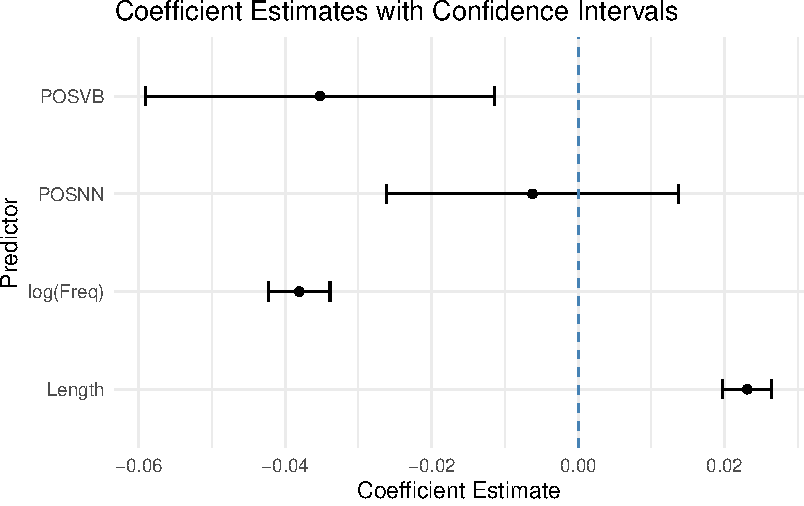
\includegraphics{Linear_regression_files/figure-pdf/unnamed-chunk-11-1.pdf}

Plot contributions of individual variable values:

\begin{Shaded}
\begin{Highlighting}[]
\CommentTok{\# Plot marginal effects}

\FunctionTok{library}\NormalTok{(}\StringTok{"effects"}\NormalTok{)}

\FunctionTok{plot}\NormalTok{(}\FunctionTok{Effect}\NormalTok{(}\StringTok{"Freq"}\NormalTok{, }\AttributeTok{mod =}\NormalTok{ rt.lm2))}
\end{Highlighting}
\end{Shaded}

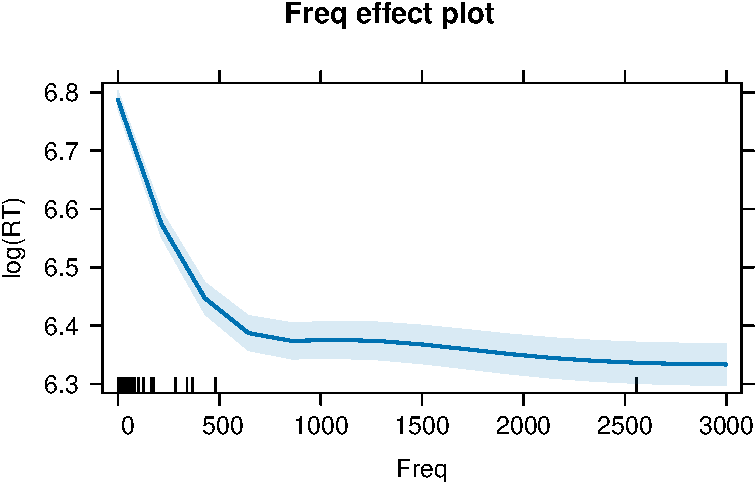
\includegraphics{Linear_regression_files/figure-pdf/unnamed-chunk-12-1.pdf}

\begin{Shaded}
\begin{Highlighting}[]
\FunctionTok{plot}\NormalTok{(}\FunctionTok{Effect}\NormalTok{(}\StringTok{"POS"}\NormalTok{, }\AttributeTok{mod =}\NormalTok{ rt.lm2))}
\end{Highlighting}
\end{Shaded}

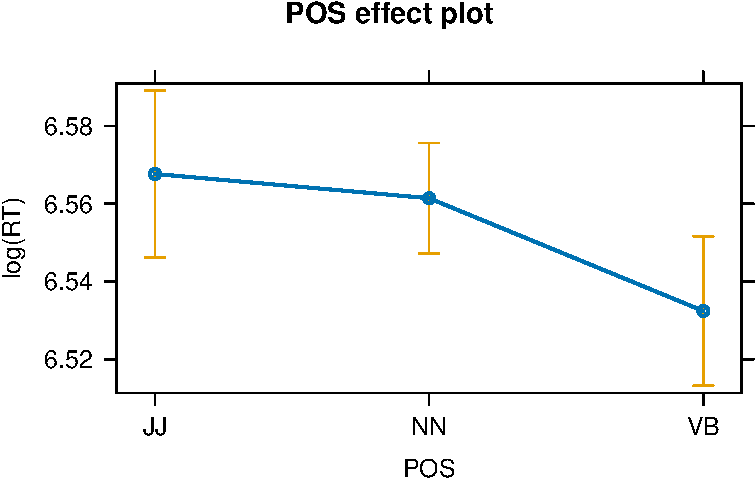
\includegraphics{Linear_regression_files/figure-pdf/unnamed-chunk-12-2.pdf}

\begin{Shaded}
\begin{Highlighting}[]
\FunctionTok{plot}\NormalTok{(}\FunctionTok{Effect}\NormalTok{(}\StringTok{"Length"}\NormalTok{, }\AttributeTok{mod =}\NormalTok{ rt.lm2))}
\end{Highlighting}
\end{Shaded}

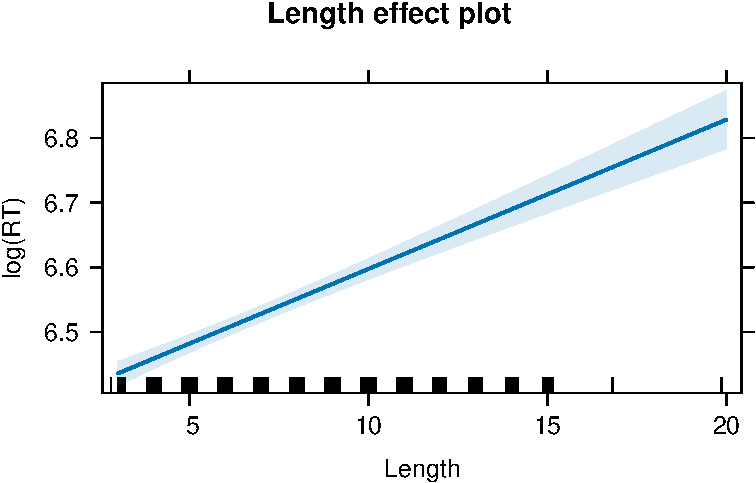
\includegraphics{Linear_regression_files/figure-pdf/unnamed-chunk-12-3.pdf}

\section{Model assumptions and
diagnostics}\label{model-assumptions-and-diagnostics}

As a parametric method, linear regression makes numerous assumptions
about the training data. It is, therefore, essential to run further
tests to rule out possible violations. Among other things, the model
assumptions include:

\begin{itemize}
\item
  A \textbf{linear relationship} between the response and the
  quantitative predictors: The residuals should not display a clear
  pattern. For this reason, it is recommended to use component residual
  plots (e.g., \texttt{crPlot()} from the \texttt{car} library) for the
  visual identification of potentially non-linear trends.
\item
  \textbf{No heteroscedasticity} (i.e, non-constant variance of error
  terms): Visually, a violation of this assumption becomes apparent if
  the residuals form a funnel-like shape. It is also possible to conduct
  a non-constant variance test \texttt{ncvTest()}: If it returns
  \(p\)-values \textless{} 0.05, this suggests non-constant variance.
\item
  \textbf{No multicollinearity}: Predictors should not be correlated
  with each other. In the model data, correlated variables have
  unusually high standard errors, thereby decreasing the explanatory
  power of both the coefficients and the model as a whole. Another
  diagnostic measure are variance inflation factors (VIF-scores);
  predictors with VIF scores \textgreater{} 5 are potentially collinear.
  They can be computed using the \texttt{vif()} function.
\item
  \textbf{Normally distributed residuals}: The residuals should follow
  the normal distribution. Usually, a visual inspection using
  \texttt{qqnorm()} is sufficient, but the Shapiro-Wilke test
  \texttt{shapiro.test()} can also be run on the model residuals. Note
  that a \(p\)-value below 0.05 provides evidence for non-normality.
\end{itemize}

\begin{tcolorbox}[enhanced jigsaw, toprule=.15mm, opacitybacktitle=0.6, coltitle=black, arc=.35mm, colback=white, title=\textcolor{quarto-callout-important-color}{\faExclamation}\hspace{0.5em}{Important}, titlerule=0mm, toptitle=1mm, bottomtitle=1mm, breakable, rightrule=.15mm, opacityback=0, bottomrule=.15mm, leftrule=.75mm, colframe=quarto-callout-important-color-frame, left=2mm, colbacktitle=quarto-callout-important-color!10!white]

Beside the points mentioned above, it is always recommend to examine the
model with regard to

\begin{itemize}
\item
  \textbf{outliers} that might skew the regression estimates,
\item
  \textbf{interactions}, i.e., combined effects of predictors, and
\item
  \textbf{overfitting}, which results in poor model performance outside
  the training data.
\end{itemize}

\end{tcolorbox}

\chapter{Logistic Regression}\label{logistic-regression}

\section{Recommended reading}\label{recommended-reading-5}

\begin{quote}
This unit is based on James et al. (2021: Chapter 4) and Levshina (2015:
Chapter 12). For an in-depth introduction, see Hosmer \& Lemeshow
(2008).
\end{quote}

\section{Preparation}\label{preparation-8}

Consider the data from Buskin's (n.d.) corpus-study on subject pronoun
realisation:

\begin{Shaded}
\begin{Highlighting}[]
\CommentTok{\# Load libraries}
\FunctionTok{library}\NormalTok{(}\StringTok{"tidyverse"}\NormalTok{)}
\FunctionTok{library}\NormalTok{(}\StringTok{"rms"}\NormalTok{) }\CommentTok{\# For regression modelling}

\CommentTok{\# Load data}
\NormalTok{data\_pro }\OtherTok{\textless{}{-}} \FunctionTok{read\_csv}\NormalTok{(}\StringTok{"data/Buskin\_pronoun\_data.csv"}\NormalTok{, }\AttributeTok{sep =} \StringTok{","}\NormalTok{, }\AttributeTok{header =} \ConstantTok{TRUE}\NormalTok{)}
\end{Highlighting}
\end{Shaded}

\begin{itemize}
\item
  \textbf{Target variable}:

  \begin{itemize}
  \tightlist
  \item
    \texttt{Reference} (`overt', `null')
  \end{itemize}
\item
  \textbf{Explanatory variables}:

  \begin{itemize}
  \item
    \texttt{Person} (`1.p.', `2.p', `3.p' as well as the dummy pronouns
    `it' and `there')
  \item
    \texttt{Register} (the text category in the International Corpus of
    English; `S1A' are informal conversations, whereas `S1B' comprises
    formal class lessons)
  \item
    \texttt{Variety} (British English `GB', Singapore English `SING' and
    Hong Kong English `HK') and
  \item
    \texttt{Referentiality} (`referential' with an identifiable referent
    or `non-referential' with no/generic reference)
  \end{itemize}
\end{itemize}

\begin{Shaded}
\begin{Highlighting}[]
\FunctionTok{head}\NormalTok{(data\_pro)}
\end{Highlighting}
\end{Shaded}

\begin{verbatim}
  Reference Person Register Variety Referentiality
1     overt      3      S1A      GB    referential
2     overt      3      S1A      GB    referential
3     overt      3      S1A      GB    referential
4     overt      3      S1A      GB    referential
5     overt      3      S1A      GB    referential
6     overt      3      S1A      GB    referential
\end{verbatim}

\begin{Shaded}
\begin{Highlighting}[]
\FunctionTok{table}\NormalTok{(data\_pro}\SpecialCharTok{$}\NormalTok{Reference)}
\end{Highlighting}
\end{Shaded}

\begin{verbatim}

 null overt 
  174  4664 
\end{verbatim}

\subsection{Descriptive overview}\label{descriptive-overview-1}

\begin{Shaded}
\begin{Highlighting}[]
\CommentTok{\# Raw data for Ref x Reg x Var}
\NormalTok{data\_pro }\SpecialCharTok{\%\textgreater{}\%} 
  \FunctionTok{count}\NormalTok{(Reference, Register, Variety) }\SpecialCharTok{\%\textgreater{}\%} 
  \FunctionTok{filter}\NormalTok{(Reference }\SpecialCharTok{==} \StringTok{"null"}\NormalTok{) }\SpecialCharTok{\%\textgreater{}\%} 
  \FunctionTok{mutate}\NormalTok{(}\AttributeTok{pct =}\NormalTok{ n}\SpecialCharTok{/}\FunctionTok{sum}\NormalTok{(n) }\SpecialCharTok{*} \DecValTok{100}\NormalTok{) }\OtherTok{{-}\textgreater{}}\NormalTok{ pro\_stats1}

\CommentTok{\# Raw data for Ref x Per x Var}
\NormalTok{data\_pro }\SpecialCharTok{\%\textgreater{}\%} 
  \FunctionTok{count}\NormalTok{(Reference, Person, Variety) }\SpecialCharTok{\%\textgreater{}\%} 
  \FunctionTok{filter}\NormalTok{(Reference }\SpecialCharTok{==} \StringTok{"null"}\NormalTok{) }\SpecialCharTok{\%\textgreater{}\%} 
  \FunctionTok{mutate}\NormalTok{(}\AttributeTok{pct =}\NormalTok{ n}\SpecialCharTok{/}\FunctionTok{sum}\NormalTok{(n) }\SpecialCharTok{*} \DecValTok{100}\NormalTok{) }\OtherTok{{-}\textgreater{}}\NormalTok{ pro\_stats2}

\CommentTok{\# Raw data for Ref x Referent. x Var}
\NormalTok{data\_pro }\SpecialCharTok{\%\textgreater{}\%} 
  \FunctionTok{count}\NormalTok{(Reference, Referentiality, Variety) }\SpecialCharTok{\%\textgreater{}\%} 
  \FunctionTok{filter}\NormalTok{(Reference }\SpecialCharTok{==} \StringTok{"null"}\NormalTok{) }\SpecialCharTok{\%\textgreater{}\%} 
  \FunctionTok{mutate}\NormalTok{(}\AttributeTok{pct =}\NormalTok{ n}\SpecialCharTok{/}\FunctionTok{sum}\NormalTok{(n) }\SpecialCharTok{*} \DecValTok{100}\NormalTok{) }\OtherTok{{-}\textgreater{}}\NormalTok{ pro\_stats3}

\CommentTok{\# Plot 1}

\NormalTok{pro\_stats1 }\SpecialCharTok{\%\textgreater{}\%}
  \FunctionTok{ggplot}\NormalTok{(}\FunctionTok{aes}\NormalTok{(}\AttributeTok{x =}\NormalTok{ Variety, }\AttributeTok{y =}\NormalTok{ pct, }\AttributeTok{color =}\NormalTok{ Register)) }\SpecialCharTok{+}
  \FunctionTok{geom\_point}\NormalTok{(}\AttributeTok{size =} \DecValTok{3}\NormalTok{) }\SpecialCharTok{+}
  \FunctionTok{theme\_minimal}\NormalTok{() }\SpecialCharTok{+}
  \FunctionTok{labs}\NormalTok{(}
    \AttributeTok{title =} \StringTok{"Null subjects by Variety and Register"}\NormalTok{,}
    \AttributeTok{y =} \StringTok{"Proportion of null subjects"}
\NormalTok{  )}
\end{Highlighting}
\end{Shaded}

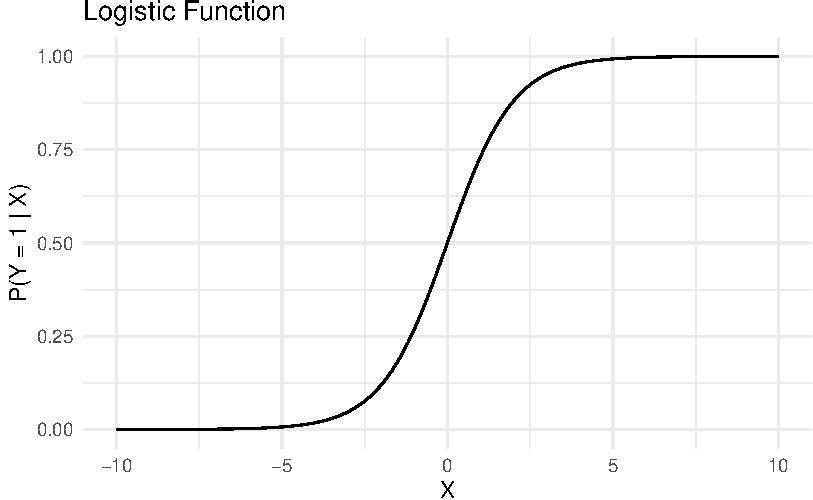
\includegraphics{Logistic_regression_files/figure-pdf/unnamed-chunk-4-1.pdf}

\begin{Shaded}
\begin{Highlighting}[]
\CommentTok{\# Plot 2}

\NormalTok{pro\_stats2 }\SpecialCharTok{\%\textgreater{}\%}
  \FunctionTok{ggplot}\NormalTok{(}\FunctionTok{aes}\NormalTok{(}\AttributeTok{x =}\NormalTok{ Variety, }\AttributeTok{y =}\NormalTok{ pct, }\AttributeTok{color =}\NormalTok{ Person)) }\SpecialCharTok{+}
  \FunctionTok{geom\_point}\NormalTok{(}\AttributeTok{size =} \DecValTok{3}\NormalTok{) }\SpecialCharTok{+}
  \FunctionTok{theme\_minimal}\NormalTok{() }\SpecialCharTok{+}
  \FunctionTok{labs}\NormalTok{(}
    \AttributeTok{title =} \StringTok{"Null subjects by Variety and Person"}\NormalTok{,}
    \AttributeTok{y =} \StringTok{"Proportion of null subjects"}
\NormalTok{  )}
\end{Highlighting}
\end{Shaded}

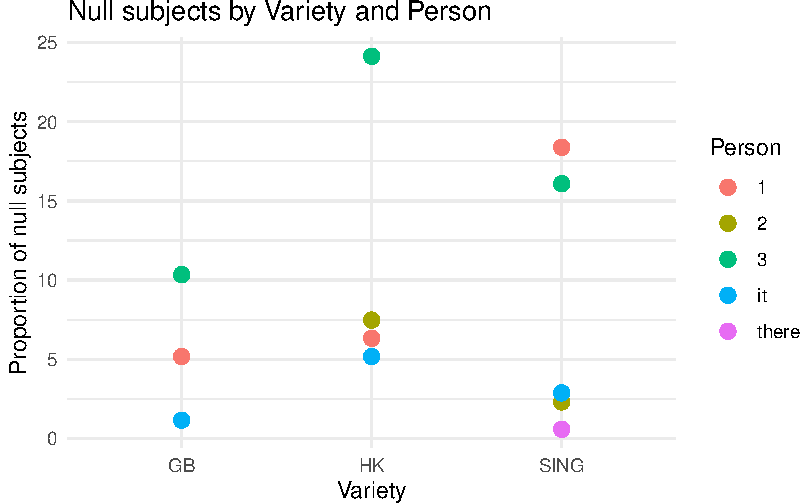
\includegraphics{Logistic_regression_files/figure-pdf/unnamed-chunk-4-2.pdf}

\begin{Shaded}
\begin{Highlighting}[]
\CommentTok{\# Plot 3}

\NormalTok{pro\_stats3 }\SpecialCharTok{\%\textgreater{}\%}
  \FunctionTok{ggplot}\NormalTok{(}\FunctionTok{aes}\NormalTok{(}\AttributeTok{x =}\NormalTok{ Variety, }\AttributeTok{y =}\NormalTok{ pct, }\AttributeTok{color =}\NormalTok{ Referentiality)) }\SpecialCharTok{+}
  \FunctionTok{geom\_point}\NormalTok{(}\AttributeTok{size =} \DecValTok{3}\NormalTok{) }\SpecialCharTok{+}
  \FunctionTok{theme\_minimal}\NormalTok{() }\SpecialCharTok{+}
  \FunctionTok{labs}\NormalTok{(}
    \AttributeTok{title =} \StringTok{"Null subjects by Variety and Referentiality"}\NormalTok{,}
    \AttributeTok{y =} \StringTok{"Proportion of null subjects"}
\NormalTok{  )}
\end{Highlighting}
\end{Shaded}

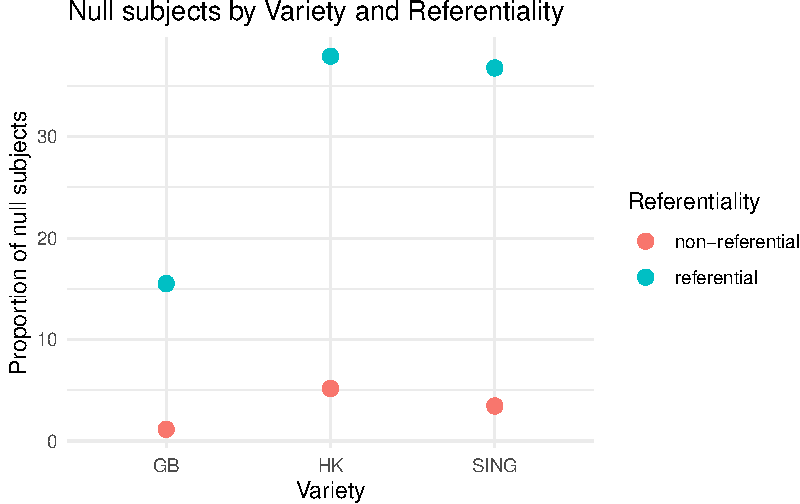
\includegraphics{Logistic_regression_files/figure-pdf/unnamed-chunk-4-3.pdf}

\section{Logistic regression}\label{logistic-regression-1}

\begin{itemize}
\item
  In contrast to linear regression, logistic regression models a
  \textbf{qualitative response variable} \(Y\) (here:
  \texttt{Reference}) with two outcomes as a function of the independent
  variables \(X_p\) (\texttt{Register}, Variety etc.). The goal is to
  predict a value for \(Y\).
\item
  For a given observation, the model should predict either a specific
  category of \(Y\) (e.g., \texttt{Reference\ =\ overt} or
  \texttt{Reference\ =\ null}) or provide a probability estimation of a
  particular outcome (e.g., the probability of
  \texttt{Reference\ =\ null}).
\item
  The probability that \texttt{Reference\ =\ null} given a predictor
  (e.g., \texttt{Register}) can be written as
  \(P(\text{Reference} = \text{null} \mid \text{Register})\) or more
  simply as \(p(\text{Register})\).
\item
  A core component of logistic regression is the \textbf{logistic
  function}. The rationale for using it is that the output of the
  function will always lie between \(0\) and \(1\), and it will always
  denote a \textbf{probability}.
\end{itemize}

\includegraphics{Logistic_regression_files/figure-pdf/unnamed-chunk-5-1.pdf}

\subsection{The logistic model}\label{the-logistic-model}

Assuming a binary response variable \(Y\) with the values 1 and 0 and a
single predictor \(X\), we can model the probability
\(P(Y = 1\vert X) = p(X)\) as

\[
p(X) = \frac{e^{\beta_0 + \beta_1X}}{1 + e^{\beta_0 + \beta_1X}}.
\]

Note that \(e \approx 2.71828\). This expression is equivalent to

\[
\log\left(\frac{p(X)}{1-p(X)}\right) = \beta_0 + \beta_1X.
\]

The fraction \(\frac{p(X)}{1-p(X)}\) represents the \textbf{odds}, which
stand for to the probability of one outcome (e.g.,
\texttt{Reference\ =\ null}) compared to the other (e.g.,
\texttt{Reference\ =\ overt}). Their logarithmic transformation are the
\textbf{log odds} (or \textbf{logits}) of a model. When interpreting the
output of a logistic model, note that

\begin{itemize}
\item
  positive log odds indicate an \textbf{increase} in \(p(X)\), whereas
\item
  negative log odds indicate a \textbf{decrease} in \(p(X)\).
\end{itemize}

If \(X = \text{Register}\), then our model has the form:

\[
\log\left(\frac{P(\text{Reference} = \text{null} \mid \text{Register})}{1- P(\text{Reference} = \text{null} \mid \text{Register})}\right) = \beta_0 + \beta_1\text{Register}
\]

\subsection{Multiple logistic
regression}\label{multiple-logistic-regression}

If more than one predictor is included, the above equations can be
expanded so as to take into account \(p\) slopes \(\beta_p\) for \(p\)
independent variables \(X_p\).

\[
p(X) = \frac{e^{\beta_0 + \beta_1X_1 + ... +  \beta_pX_p}}{1 + e^{\beta_0 + \beta_1X_1 + ... + \beta_pX_p}}.
\] Thus, the log odds correspond to the sum of \(\beta_pX_p\),

\[
\begin{aligned}
\log\left(\frac{p(X)}{1-p(X)}\right) &= \beta_0 + \beta_1X_1 + ... +  \beta_pX_p \\
& = \beta_0 + \sum_{i=1}^{p} \beta_i X_i
\end{aligned}
\] respectively.

\subsection{Odds ratios}\label{odds-ratios}

To assess the strength of an effect, it is instructive to examine the
\textbf{odds ratios} that correspond to the model coefficients. Odds
ratios (OR) are defined as

\[
OR(X_1) = e^{\beta_1}.
\]

Essentially, the OR describes the ratio between two odds with respect to
another independent variable. This is illustrated for \texttt{Reference}
given \texttt{Register} below:

\[
\text{OR}(\text{Reference} \mid \text{Register}) = \frac{\frac{P(\text{Reference} = \text{null} \mid \text{Register} = \text{S1A})}{P(\text{Reference} = \text{overt} \mid \text{Register} = \text{S1A})}}{\frac{P(\text{Reference} = \text{null} \mid \text{Register} = \text{S1B})}{P(\text{Reference} = \text{overt} \mid \text{Register} = \text{S1B})}}
\] Read as: `\textbf{The ratio between} the probability of a null
vs.~overt object in S1A \textbf{and} the probability of a null vs.~overt
object in S1B'.

\section{Workflow in R}\label{workflow-in-r-2}

\subsection{Step 1: Research question and
hypotheses}\label{step-1-research-question-and-hypotheses}

How do the intra- and extra-linguistic variables suggested in the
literature affect subject pronoun realisation (Definite Null
Instantiation) in British English, Singapore English and Hong Kong
English?

Given a significance level \(\alpha = 0.05\), the hypotheses are: \[ 
\begin{aligned}
H_0: & \quad \text{None of the predictor coefficients deviate from 0}.\\
H_1: & \quad \text{At least one predictor coefficient deviates from 0}.
\end{aligned}
\]

These can be restated mathematically as:

\[ 
\begin{aligned}
H_0: & \quad \beta_1 = \beta_2 = \cdots = \beta_p = 0 \\
H_1: & \quad \text{At least one } \beta_i \neq 0 \text{ for } i \in \{1, 2, \ldots, p\}
\end{aligned} \]

\subsection{Step 2: Convert to factors and specify reference
levels}\label{step-2-convert-to-factors-and-specify-reference-levels}

The next step involves specifying \textbf{reference levels} for all
categorical variables. This step is very important because it will
directly impact the parameter estimation and, consequently, influence
our interpretation of the model output.

\begin{itemize}
\item
  The reference level of the response is usually chosen such that it
  corresponds to the \textbf{unmarked or most frequent case}. Since
  overt pronouns are much more common in the data, the reference level
  of the \texttt{Reference} variable will be set to
  \texttt{Reference\ =\ overt}. This way, the model coefficients will
  directly represent the probability of the \textbf{null}
  \textbf{subject} variant (i.e., the special case) given certain
  predictor configurations.
\item
  The \textbf{predictor levels} need to be specified as well. Among
  other things, we are interested in how the Asian Englishes pattern
  relative to British English. Therefore, we will define British English
  as the baseline for comparison.
\end{itemize}

We will use the following specifications:

\begin{longtable}[]{@{}
  >{\raggedright\arraybackslash}p{(\columnwidth - 4\tabcolsep) * \real{0.2639}}
  >{\raggedright\arraybackslash}p{(\columnwidth - 4\tabcolsep) * \real{0.3611}}
  >{\raggedright\arraybackslash}p{(\columnwidth - 4\tabcolsep) * \real{0.3750}}@{}}
\toprule\noalign{}
\begin{minipage}[b]{\linewidth}\raggedright
\textbf{Variable}
\end{minipage} & \begin{minipage}[b]{\linewidth}\raggedright
\textbf{Factor Levels}
\end{minipage} & \begin{minipage}[b]{\linewidth}\raggedright
\textbf{Preferred Reference level}
\end{minipage} \\
\midrule\noalign{}
\endhead
\bottomrule\noalign{}
\endlastfoot
Register & S1A, S1B & S1A \\
Variety & GB, SING, HK & GB \\
Person & 1, 2, 3, \emph{it}, \emph{there} & 3 \\
Referentiality & referential, non-referential & referential \\
\end{longtable}

\begin{Shaded}
\begin{Highlighting}[]
\CommentTok{\# Store "Reference" as factor}
\NormalTok{data\_pro}\SpecialCharTok{$}\NormalTok{Reference }\OtherTok{\textless{}{-}} \FunctionTok{as.factor}\NormalTok{(data\_pro}\SpecialCharTok{$}\NormalTok{Reference)}

\DocumentationTok{\#\# Specify reference level (the \textquotesingle{}unmarked\textquotesingle{} case)}
\NormalTok{data\_pro}\SpecialCharTok{$}\NormalTok{Reference }\OtherTok{\textless{}{-}} \FunctionTok{relevel}\NormalTok{(data\_pro}\SpecialCharTok{$}\NormalTok{Reference, }\StringTok{"overt"}\NormalTok{)}

\DocumentationTok{\#\# Print levels}
\FunctionTok{levels}\NormalTok{(data\_pro}\SpecialCharTok{$}\NormalTok{Reference)}
\end{Highlighting}
\end{Shaded}

\begin{verbatim}
[1] "overt" "null" 
\end{verbatim}

Repeat the procedure for the remaining categorical variables.

\begin{Shaded}
\begin{Highlighting}[]
\CommentTok{\# Store "Register" as factor}
\NormalTok{data\_pro}\SpecialCharTok{$}\NormalTok{Register }\OtherTok{\textless{}{-}} \FunctionTok{as.factor}\NormalTok{(data\_pro}\SpecialCharTok{$}\NormalTok{Register)}

\DocumentationTok{\#\# Specify reference level}
\NormalTok{data\_pro}\SpecialCharTok{$}\NormalTok{Register }\OtherTok{\textless{}{-}} \FunctionTok{relevel}\NormalTok{(data\_pro}\SpecialCharTok{$}\NormalTok{Register, }\StringTok{"S1A"}\NormalTok{)}

\CommentTok{\# Store "Variety" as factor}
\NormalTok{data\_pro}\SpecialCharTok{$}\NormalTok{Variety }\OtherTok{\textless{}{-}} \FunctionTok{as.factor}\NormalTok{(data\_pro}\SpecialCharTok{$}\NormalTok{Variety)}

\DocumentationTok{\#\# Specify reference level}
\NormalTok{data\_pro}\SpecialCharTok{$}\NormalTok{Variety }\OtherTok{\textless{}{-}} \FunctionTok{relevel}\NormalTok{(data\_pro}\SpecialCharTok{$}\NormalTok{Variety, }\StringTok{"GB"}\NormalTok{)}

\CommentTok{\# Store "Person" as factor}
\NormalTok{data\_pro}\SpecialCharTok{$}\NormalTok{Person }\OtherTok{\textless{}{-}} \FunctionTok{as.factor}\NormalTok{(data\_pro}\SpecialCharTok{$}\NormalTok{Person)}

\DocumentationTok{\#\# Specify reference level}
\NormalTok{data\_pro}\SpecialCharTok{$}\NormalTok{Person }\OtherTok{\textless{}{-}} \FunctionTok{relevel}\NormalTok{(data\_pro}\SpecialCharTok{$}\NormalTok{Person, }\StringTok{"3"}\NormalTok{)}

\CommentTok{\# Store "Referentiality" as factor}
\NormalTok{data\_pro}\SpecialCharTok{$}\NormalTok{Referentiality }\OtherTok{\textless{}{-}} \FunctionTok{as.factor}\NormalTok{(data\_pro}\SpecialCharTok{$}\NormalTok{Referentiality)}

\DocumentationTok{\#\# Specify reference level}
\NormalTok{data\_pro}\SpecialCharTok{$}\NormalTok{Referentiality }\OtherTok{\textless{}{-}} \FunctionTok{relevel}\NormalTok{(data\_pro}\SpecialCharTok{$}\NormalTok{Referentiality, }\StringTok{"referential"}\NormalTok{)}
\end{Highlighting}
\end{Shaded}

\subsection{Step 3: Fit the model}\label{step-3-fit-the-model}

There are two functions that can fit logistic models in R:
\texttt{lrm()} and \texttt{glm()}.

\begin{tcolorbox}[enhanced jigsaw, toprule=.15mm, opacitybacktitle=0.6, coltitle=black, arc=.35mm, colback=white, title=\textcolor{quarto-callout-note-color}{\faInfo}\hspace{0.5em}{Note}, titlerule=0mm, toptitle=1mm, bottomtitle=1mm, breakable, rightrule=.15mm, opacityback=0, bottomrule=.15mm, leftrule=.75mm, colframe=quarto-callout-note-color-frame, left=2mm, colbacktitle=quarto-callout-note-color!10!white]

The model formula below does not include \texttt{Referentiality} because
several intermediary steps revealed it to be almost completely
irrelevant for predicting \texttt{Reference}. In addition, the existing
(and significant) interaction \texttt{Variety:Person} has been excluded
to improve the interpretability of the model.

\end{tcolorbox}

\begin{Shaded}
\begin{Highlighting}[]
\CommentTok{\# With lrm(); requires library("rms")}

\CommentTok{\# Fit interaction model}
\NormalTok{Reference.lrm }\OtherTok{\textless{}{-}} \FunctionTok{lrm}\NormalTok{(Reference }\SpecialCharTok{\textasciitilde{}}\NormalTok{ Register }\SpecialCharTok{+}\NormalTok{ Variety }\SpecialCharTok{+}\NormalTok{ Register}\SpecialCharTok{:}\NormalTok{Variety }\SpecialCharTok{+}\NormalTok{ Person, }\AttributeTok{data =}\NormalTok{ data\_pro)}

\CommentTok{\# View model statistics}
\NormalTok{Reference.lrm}
\end{Highlighting}
\end{Shaded}

\begin{verbatim}
Logistic Regression Model

lrm(formula = Reference ~ Register + Variety + Register:Variety + 
    Person, data = data_pro)

                       Model Likelihood      Discrimination    Rank Discrim.    
                             Ratio Test             Indexes          Indexes    
Obs          4838    LR chi2     120.43      R2       0.092    C       0.729    
 overt       4664    d.f.             9     R2(9,4838)0.023    Dxy     0.458    
 null         174    Pr(> chi2) <0.0001    R2(9,503.2)0.199    gamma   0.488    
max |deriv| 4e-10                            Brier    0.034    tau-a   0.032    

                            Coef    S.E.   Wald Z Pr(>|Z|)
Intercept                   -3.4132 0.2746 -12.43 <0.0001 
Register=S1B                 0.0269 0.3807   0.07 0.9437  
Variety=HK                   0.6712 0.3174   2.11 0.0345  
Variety=SING                 1.1193 0.2959   3.78 0.0002  
Person=1                    -0.8807 0.1811  -4.86 <0.0001 
Person=2                    -1.6441 0.2695  -6.10 <0.0001 
Person=it                    0.7897 0.2978   2.65 0.0080  
Person=there                -2.5641 1.0095  -2.54 0.0111  
Register=S1B * Variety=HK    0.6035 0.4521   1.34 0.1819  
Register=S1B * Variety=SING -0.4753 0.4688  -1.01 0.3107  
\end{verbatim}

\begin{Shaded}
\begin{Highlighting}[]
\CommentTok{\# With (glm); available in base R}
\CommentTok{\# Note the additional "family" argument!}
\NormalTok{Reference.glm }\OtherTok{\textless{}{-}} \FunctionTok{glm}\NormalTok{(Reference }\SpecialCharTok{\textasciitilde{}}\NormalTok{ Register }\SpecialCharTok{+}\NormalTok{ Variety }\SpecialCharTok{+}\NormalTok{ Register}\SpecialCharTok{:}\NormalTok{Variety }\SpecialCharTok{+}\NormalTok{ Person, }\AttributeTok{data =}\NormalTok{ data\_pro, }\AttributeTok{family =} \StringTok{"binomial"}\NormalTok{)}

\CommentTok{\# View model statistics}
\FunctionTok{summary}\NormalTok{(Reference.glm)}
\end{Highlighting}
\end{Shaded}

\begin{tcolorbox}[enhanced jigsaw, toprule=.15mm, opacitybacktitle=0.6, coltitle=black, arc=.35mm, colback=white, title=\textcolor{quarto-callout-tip-color}{\faLightbulb}\hspace{0.5em}{Stepwise variable selection}, titlerule=0mm, toptitle=1mm, bottomtitle=1mm, breakable, rightrule=.15mm, opacityback=0, bottomrule=.15mm, leftrule=.75mm, colframe=quarto-callout-tip-color-frame, left=2mm, colbacktitle=quarto-callout-tip-color!10!white]

With the function \texttt{drop1()}, it is possible to successively
remove variables from the complex model to ascertain which ones improve
the model significantly (i.e., decrease the deviance and AIC scores).

\begin{Shaded}
\begin{Highlighting}[]
\FunctionTok{drop1}\NormalTok{(Reference.glm, }\AttributeTok{test =} \StringTok{"Chisq"}\NormalTok{)}
\end{Highlighting}
\end{Shaded}

\end{tcolorbox}

\subsection{Step 4: Confidence intervals and odds
ratios}\label{step-4-confidence-intervals-and-odds-ratios}

\begin{Shaded}
\begin{Highlighting}[]
\CommentTok{\# Tidy the model output}
\NormalTok{tidy\_model }\OtherTok{\textless{}{-}} \FunctionTok{tidy}\NormalTok{(Reference.glm, }\AttributeTok{conf.int =} \ConstantTok{TRUE}\NormalTok{)}

\CommentTok{\# Remove intercept, compute odds ratios and their CIs}
\NormalTok{tidy\_model }\OtherTok{\textless{}{-}}\NormalTok{ tidy\_model }\SpecialCharTok{\%\textgreater{}\%} 
  \FunctionTok{filter}\NormalTok{(term }\SpecialCharTok{!=} \StringTok{"(Intercept)"}\NormalTok{) }\SpecialCharTok{\%\textgreater{}\%} 
  \FunctionTok{mutate}\NormalTok{(}
    \AttributeTok{odds\_ratio =} \FunctionTok{exp}\NormalTok{(estimate),}
    \AttributeTok{odds.conf.low =} \FunctionTok{exp}\NormalTok{(conf.low),}
    \AttributeTok{odds.conf.high =} \FunctionTok{exp}\NormalTok{(conf.high)}
\NormalTok{  )}
\end{Highlighting}
\end{Shaded}

\subsection{Step 5: Visualise the
model}\label{step-5-visualise-the-model}

\begin{Shaded}
\begin{Highlighting}[]
\CommentTok{\# Create the coefficient plot}
\FunctionTok{ggplot}\NormalTok{(tidy\_model, }\FunctionTok{aes}\NormalTok{(}\AttributeTok{x =}\NormalTok{ estimate, }\AttributeTok{y =}\NormalTok{ term)) }\SpecialCharTok{+}
  \FunctionTok{geom\_point}\NormalTok{() }\SpecialCharTok{+}
  \FunctionTok{geom\_errorbarh}\NormalTok{(}\FunctionTok{aes}\NormalTok{(}\AttributeTok{xmin =}\NormalTok{ conf.low, }\AttributeTok{xmax =}\NormalTok{ conf.high), }\AttributeTok{height =} \FloatTok{0.2}\NormalTok{) }\SpecialCharTok{+}
  \FunctionTok{geom\_vline}\NormalTok{(}\AttributeTok{xintercept =} \DecValTok{0}\NormalTok{, }\AttributeTok{linetype =} \StringTok{"dashed"}\NormalTok{, }\AttributeTok{color =} \StringTok{"steelblue"}\NormalTok{) }\SpecialCharTok{+}
  \FunctionTok{theme\_minimal}\NormalTok{() }\SpecialCharTok{+}
  \FunctionTok{labs}\NormalTok{(}
    \AttributeTok{x =} \StringTok{"Coefficient Estimate (log{-}odds)"}\NormalTok{,}
    \AttributeTok{y =} \StringTok{"Predictor"}\NormalTok{,}
    \AttributeTok{title =} \StringTok{"Coefficient Estimates with Confidence Intervals"}\NormalTok{,}
    \AttributeTok{caption =} \StringTok{"*Note that the CIs of singificant predictors do not include 0."}
\NormalTok{  )}
\end{Highlighting}
\end{Shaded}

\includegraphics{Logistic_regression_files/figure-pdf/unnamed-chunk-12-1.pdf}

\begin{Shaded}
\begin{Highlighting}[]
\CommentTok{\# Plot odds ratios}
\FunctionTok{ggplot}\NormalTok{(tidy\_model, }\FunctionTok{aes}\NormalTok{(}\AttributeTok{x =} \FunctionTok{exp}\NormalTok{(estimate), }\AttributeTok{y =}\NormalTok{ term)) }\SpecialCharTok{+}
  \FunctionTok{geom\_point}\NormalTok{() }\SpecialCharTok{+}
  \FunctionTok{geom\_errorbarh}\NormalTok{(}\FunctionTok{aes}\NormalTok{(}\AttributeTok{xmin =}\NormalTok{ odds.conf.low, }\AttributeTok{xmax =}\NormalTok{ odds.conf.high), }\AttributeTok{height =} \FloatTok{0.2}\NormalTok{) }\SpecialCharTok{+}
  \FunctionTok{geom\_vline}\NormalTok{(}\AttributeTok{xintercept =} \DecValTok{1}\NormalTok{, }\AttributeTok{linetype =} \StringTok{"dashed"}\NormalTok{, }\AttributeTok{color =} \StringTok{"steelblue"}\NormalTok{) }\SpecialCharTok{+}
  \FunctionTok{theme\_minimal}\NormalTok{() }\SpecialCharTok{+}
  \FunctionTok{labs}\NormalTok{(}
    \AttributeTok{x =} \StringTok{"Coefficient Estimate (odds ratios)"}\NormalTok{,}
    \AttributeTok{y =} \StringTok{"Predictor"}\NormalTok{,}
    \AttributeTok{title =} \StringTok{"Odds ratios with Confidence Intervals"}\NormalTok{,}
    \AttributeTok{caption =} \StringTok{"*Note that the CIs of singificant predictors do not include 1."}
\NormalTok{  )}
\end{Highlighting}
\end{Shaded}

\includegraphics{Logistic_regression_files/figure-pdf/unnamed-chunk-12-2.pdf}

\begin{Shaded}
\begin{Highlighting}[]
\CommentTok{\# Plot marginal effects; y{-}axis = log odds of a null vs. overt subject}
\FunctionTok{plot}\NormalTok{(}\FunctionTok{Effect}\NormalTok{(}\StringTok{"Register"}\NormalTok{, }\AttributeTok{mod =}\NormalTok{ Reference.glm)) }
\end{Highlighting}
\end{Shaded}

\includegraphics{Logistic_regression_files/figure-pdf/unnamed-chunk-12-3.pdf}

\begin{Shaded}
\begin{Highlighting}[]
\FunctionTok{plot}\NormalTok{(}\FunctionTok{Effect}\NormalTok{(}\StringTok{"Variety"}\NormalTok{, }\AttributeTok{mod =}\NormalTok{ Reference.glm))}
\end{Highlighting}
\end{Shaded}

\includegraphics{Logistic_regression_files/figure-pdf/unnamed-chunk-12-4.pdf}

\begin{Shaded}
\begin{Highlighting}[]
\FunctionTok{plot}\NormalTok{(}\FunctionTok{Effect}\NormalTok{(}\StringTok{"Person"}\NormalTok{, }\AttributeTok{mod =}\NormalTok{ Reference.glm))}
\end{Highlighting}
\end{Shaded}

\includegraphics{Logistic_regression_files/figure-pdf/unnamed-chunk-12-5.pdf}

\begin{Shaded}
\begin{Highlighting}[]
\CommentTok{\# Plot interactions}
\FunctionTok{plot}\NormalTok{(}\FunctionTok{Effect}\NormalTok{(}\AttributeTok{focal.predictors =} \FunctionTok{c}\NormalTok{(}\StringTok{"Register"}\NormalTok{, }\StringTok{"Variety"}\NormalTok{), }\AttributeTok{mod =}\NormalTok{ Reference.glm))}
\end{Highlighting}
\end{Shaded}

\includegraphics{Logistic_regression_files/figure-pdf/unnamed-chunk-12-6.pdf}

\subsection{Step 6: Interpret the
model}\label{step-6-interpret-the-model}

The logistic regression model is statistically significant at
\(p < 0.001\) (\(\chi^2 = 120.43\), \(df = 9\)) and has acceptable fit
(Nagelkerke's-\(R^2\) = \(0.09\), \(C = 0.73\)).

The model coefficients indicate that null subjects are significantly
more likely in Singapore English compared to British English (Estimate =
1.12, 95\% CI {[}0.56, 1.73{]}, \(p < 0.001\)). This effect is moderate
with an \(OR\) of 3.06 (95\% CI {[}1.75, 5.64{]}), suggesting that the
probability of subject omission is elevated by a factor of approximately
3 in the Singaporean variety.

\ldots{}

\subsection{Step 7: Further model
diagnostics}\label{step-7-further-model-diagnostics}

\begin{itemize}
\tightlist
\item
  \textbf{Cross-validation}
\end{itemize}

\begin{Shaded}
\begin{Highlighting}[]
\CommentTok{\# Refit the model with additional settings}
\NormalTok{Reference.val }\OtherTok{\textless{}{-}} \FunctionTok{lrm}\NormalTok{(Reference }\SpecialCharTok{\textasciitilde{}}\NormalTok{ Register }\SpecialCharTok{+}\NormalTok{ Variety }\SpecialCharTok{+}\NormalTok{ Register}\SpecialCharTok{:}\NormalTok{Variety }\SpecialCharTok{+}\NormalTok{ Person, }\AttributeTok{data =}\NormalTok{ data\_pro, }\AttributeTok{x =}\NormalTok{ T, }\AttributeTok{y =}\NormalTok{ T)}

\CommentTok{\# Perform 200{-}fold cross{-}validation}
\NormalTok{model.validated }\OtherTok{\textless{}{-}} \FunctionTok{validate}\NormalTok{(Reference.val, }\AttributeTok{B =} \DecValTok{200}\NormalTok{); model.validated }
\end{Highlighting}
\end{Shaded}

\begin{verbatim}
          index.orig training    test optimism index.corrected   n
Dxy           0.4592   0.4711  0.4449   0.0262          0.4331 200
R2            0.0923   0.0995  0.0842   0.0153          0.0770 200
Intercept     0.0000   0.0000 -0.2545   0.2545         -0.2545 200
Slope         1.0000   1.0000  0.9141   0.0859          0.9141 200
Emax          0.0000   0.0000  0.0730   0.0730          0.0730 200
D             0.0247   0.0267  0.0225   0.0042          0.0205 200
U            -0.0004  -0.0004  0.0002  -0.0006          0.0002 200
Q             0.0251   0.0271  0.0223   0.0049          0.0202 200
B             0.0336   0.0336  0.0337  -0.0001          0.0337 200
g             1.0081   1.2181  1.0973   0.1208          0.8873 200
gp            0.0319   0.0328  0.0304   0.0025          0.0294 200
\end{verbatim}

\begin{Shaded}
\begin{Highlighting}[]
\CommentTok{\# Slope optimism should be as low possible!}
\end{Highlighting}
\end{Shaded}

\begin{itemize}
\tightlist
\item
  \textbf{Multicollinearity}
\end{itemize}

\begin{Shaded}
\begin{Highlighting}[]
\CommentTok{\# Variable inflation factors further reveal severe multicollinearity}
\FunctionTok{vif}\NormalTok{(Reference.lrm)}
\end{Highlighting}
\end{Shaded}

\begin{verbatim}
               Register=S1B                  Variety=HK 
                   5.818111                    4.006084 
               Variety=SING                    Person=1 
                   3.421687                    1.140407 
                   Person=2                   Person=it 
                   1.089502                    1.102908 
               Person=there   Register=S1B * Variety=HK 
                   1.007148                    6.218803 
Register=S1B * Variety=SING 
                   3.685075 
\end{verbatim}

\chapter{Decision trees and random
forests}\label{decision-trees-and-random-forests}

\section{Introduction}\label{introduction-1}

Decision trees and random forests are very popular
\textbf{non-parametric} methods. As such, ``they do not make explicit
assumptions about the functional form of \(f\)'\,' (James et al. 2021:
23).

In this unit, we will cover the conceptual basics of these methods as
well as their implementation in R using the \texttt{tv} data from
Levshina (2020) in addition to the \texttt{ELP} data from the unit on
Linear Regression. The libraries we will need are listed below:

\begin{Shaded}
\begin{Highlighting}[]
\CommentTok{\# Load libraries}
\FunctionTok{library}\NormalTok{(}\StringTok{"tidyverse"}\NormalTok{)}
\FunctionTok{library}\NormalTok{(}\StringTok{"readxl"}\NormalTok{)}
\FunctionTok{library}\NormalTok{(}\StringTok{"tree"}\NormalTok{) }\CommentTok{\# for CART}
\FunctionTok{library}\NormalTok{(}\StringTok{"randomForest"}\NormalTok{) }\CommentTok{\# for traditional random forests}
\FunctionTok{library}\NormalTok{(}\StringTok{"party"}\NormalTok{) }\CommentTok{\# for Conditional Inference Trees}
\FunctionTok{library}\NormalTok{(}\StringTok{"pdp"}\NormalTok{) }\CommentTok{\# for partial dependence plots}

\DocumentationTok{\#\# Reaction time data}
\NormalTok{ELP }\OtherTok{\textless{}{-}} \FunctionTok{read\_xlsx}\NormalTok{(}\StringTok{"data/ELP.xlsx"}\NormalTok{)}

\NormalTok{ELP}\SpecialCharTok{$}\NormalTok{POS }\OtherTok{\textless{}{-}} \FunctionTok{as.factor}\NormalTok{(ELP}\SpecialCharTok{$}\NormalTok{POS)}

\DocumentationTok{\#\# Levshina\textquotesingle{}s (2020) data set on T/V forms in Russian}
\NormalTok{tv }\OtherTok{\textless{}{-}} \FunctionTok{read.csv}\NormalTok{(}\StringTok{"data/Levshina\_2020\_tv\_data.csv"}\NormalTok{, }\AttributeTok{sep =} \StringTok{","}\NormalTok{, }\AttributeTok{header =} \ConstantTok{TRUE}\NormalTok{, }\AttributeTok{stringsAsFactors =} \ConstantTok{TRUE}\NormalTok{)}
\end{Highlighting}
\end{Shaded}

In the \texttt{tv} data frame, our target variable will be T/V
\texttt{Form} with the two outcomes \emph{ty} (Russian 2.p.sg.,
informal) and \emph{vy} (Russian 2.p.pl., polite).

\begin{Shaded}
\begin{Highlighting}[]
\FunctionTok{str}\NormalTok{(tv)}

\FunctionTok{head}\NormalTok{(tv)}
\end{Highlighting}
\end{Shaded}

\section{Decision trees}\label{decision-trees}

Core concepts:

\begin{itemize}
\item
  \textbf{Segmenting the feature space}: ``{[}T{]}he feature space
  (i.e., the space spanned by all predictor variables) is recursively
  partitioned into a set of rectangular areas'' (Strobl, Malley, and
  Tutz 2009: 325).
\item
  \textbf{Impurity reduction}: These simplified prediction areas should
  consist of mostly homogeneous (i.e., `pure' rather than `mixed')
  observations.
\item
  \textbf{Tree construction}: The `decisions' made when partitioning the
  training data can be visualised using tree structures. The nodes of a
  tree represent variables, the branches represent decision rules, and
  leaf nodes indicate the final outcome (e.g., a prediction).
\item
  \textbf{CART}: The original computational implementation of decision
  trees is known as the CART (Classification and Regression Trees)
  algorithm developed by Breiman (1984).
\end{itemize}

\subsection{Classification trees}\label{classification-trees}

If we are dealing with a \textbf{categorical response variable}, the
\texttt{tree()} function can be used to fit a classification tree in
accordance with Breiman's CART algorithm. For illustration, consider the
\texttt{tv} data frame. We will model the choice of the pronoun
\texttt{Form} based on the speaker's and hearer's social circle
(\texttt{Rel\_Circle}) and their difference in social class
(\texttt{Rel\_Class}).

\begin{Shaded}
\begin{Highlighting}[]
\CommentTok{\# Set random number generator for reproducibility}
\FunctionTok{set.seed}\NormalTok{(}\DecValTok{123}\NormalTok{)}

\CommentTok{\# Supply model formula}
\NormalTok{tree.tv }\OtherTok{\textless{}{-}} \FunctionTok{tree}\NormalTok{(Form }\SpecialCharTok{\textasciitilde{}}\NormalTok{ Rel\_Circle }\SpecialCharTok{+}\NormalTok{ Rel\_Class, }\AttributeTok{data =}\NormalTok{ tv)}

\CommentTok{\# View tree statistics}
\FunctionTok{summary}\NormalTok{(tree.tv)}
\end{Highlighting}
\end{Shaded}

\begin{verbatim}

Classification tree:
tree(formula = Form ~ Rel_Circle + Rel_Class, data = tv)
Number of terminal nodes:  9 
Residual mean deviance:  0.974 = 213.3 / 219 
Misclassification error rate: 0.2412 = 55 / 228 
\end{verbatim}

\begin{Shaded}
\begin{Highlighting}[]
\CommentTok{\# Visualisation}
\FunctionTok{plot}\NormalTok{(tree.tv)}

\FunctionTok{text}\NormalTok{(tree.tv, }\AttributeTok{pretty =} \DecValTok{3}\NormalTok{)}
\end{Highlighting}
\end{Shaded}

\includegraphics{Decision_trees_and_random_forests_files/figure-pdf/unnamed-chunk-4-1.pdf}

An important problem that arises during tree construction is that of
\textbf{split selection}. When should the tree split a node into two
further nodes and when not? Furthermore, when should the tree
\textbf{stop} the splitting process entirely? In this respect, CART
relies on the principle of \textbf{impurity reduction}: ``The
fundamental idea is to select each split of a subset so that the data in
each of the descendent subsets are `purer' than the data in the parent
subset'' (Breiman 1984: 23). A measure for node purity is the
\textbf{Gini index} \(G\), which is defined as

\[
G = \sum_{k=1}^{K}{\hat{p}_{mk}(1-\hat{p}_{mk}),}
\]

where \(\hat{p}_{mk}\) measures the proportion of observations of a
response level \(k\) in the \(m\)th prediction area of the training data
set. Values close to 0 are indicative of high node purity, meaning that
most observations belong to the same class (e.g., \texttt{Form\ =\ ty}).
If splitting a node no longer leads to a substantial increase in purity,
it becomes the \textbf{terminal node}, i.e., it is not split further.
This terminal node returns the tree's class prediction.

It is worth noting that modern CART implementations rely on different
splitting criteria. For instance, \textbf{Conditional Inference Trees}
use the \(p\) values of internal association tests to identify which
variables warrant further subdivision of the training data. The presence
or absence of correlation thus also determines whether or not a given
node will be terminal (for more details, see Greenwell 2022: 122).

\begin{Shaded}
\begin{Highlighting}[]
\CommentTok{\# Fitting a conditional inference tree}
\NormalTok{ctree.tv }\OtherTok{\textless{}{-}} \FunctionTok{ctree}\NormalTok{(Form }\SpecialCharTok{\textasciitilde{}}\NormalTok{ ., }\AttributeTok{data =}\NormalTok{ tv) }\CommentTok{\# dot . means \textquotesingle{}include all predictors\textquotesingle{}}

\FunctionTok{plot}\NormalTok{(ctree.tv)}
\end{Highlighting}
\end{Shaded}

\includegraphics{Decision_trees_and_random_forests_files/figure-pdf/unnamed-chunk-5-1.pdf}

\subsection{Regression trees}\label{regression-trees}

Regression trees are used for \textbf{continuous response variables}.
Instead of providing class predictions, they return the mean value of
observations in a given prediction area. The algorithm now strives to
\textbf{minimize the residual sum of squares} (\(RSS\); cf.~footnote 1
in 8. Linear Regression). Consider the regression tree for reaction
times depending on word length, frequency and part of speech:

\begin{Shaded}
\begin{Highlighting}[]
\CommentTok{\# CART tree}
\NormalTok{tree.rt }\OtherTok{\textless{}{-}} \FunctionTok{tree}\NormalTok{(RT }\SpecialCharTok{\textasciitilde{}}\NormalTok{ Length }\SpecialCharTok{+}\NormalTok{ Freq }\SpecialCharTok{+}\NormalTok{ POS, }\AttributeTok{data =}\NormalTok{ ELP)}

\FunctionTok{summary}\NormalTok{(tree.rt)}
\end{Highlighting}
\end{Shaded}

\begin{verbatim}

Regression tree:
tree(formula = RT ~ Length + Freq + POS, data = ELP)
Variables actually used in tree construction:
[1] "Freq"   "Length"
Number of terminal nodes:  10 
Residual mean deviance:  8629 = 7507000 / 870 
Distribution of residuals:
   Min. 1st Qu.  Median    Mean 3rd Qu.    Max. 
-220.10  -59.09  -11.17    0.00   49.66  397.40 
\end{verbatim}

\begin{Shaded}
\begin{Highlighting}[]
\FunctionTok{plot}\NormalTok{(tree.rt)}

\FunctionTok{text}\NormalTok{(tree.rt, }\AttributeTok{pretty =} \DecValTok{0}\NormalTok{)}
\end{Highlighting}
\end{Shaded}

\includegraphics{Decision_trees_and_random_forests_files/figure-pdf/unnamed-chunk-6-1.pdf}

\begin{Shaded}
\begin{Highlighting}[]
\CommentTok{\# Conditional inference tree}
\NormalTok{ctree.rt }\OtherTok{\textless{}{-}} \FunctionTok{ctree}\NormalTok{(RT }\SpecialCharTok{\textasciitilde{}}\NormalTok{ Length }\SpecialCharTok{+}\NormalTok{ Freq }\SpecialCharTok{+}\NormalTok{ POS, }\AttributeTok{data =}\NormalTok{ ELP) }

\FunctionTok{plot}\NormalTok{(ctree.rt)}
\end{Highlighting}
\end{Shaded}

\includegraphics{Decision_trees_and_random_forests_files/figure-pdf/unnamed-chunk-6-2.pdf}

\section{Random forests}\label{random-forests}

Random forests (Breiman 2001) belong to the class of \textbf{ensemble
methods} because they combine simpler models (e.g., individual decision
trees) into a more complex and possibly more accurate model. As part of
the RF algorithm, a great number of decision trees is trained on
bootstrapped samples of the training data.

So far, random forests are essentially identical with \textbf{Bagging}
(= bootstrap aggregation); however, an important additional
characteristic of the RF algorithm is that only \textbf{a random subset
of the predictors} is taken into consideration at each split. According
to (Strobl, Malley, and Tutz 2009: 332), the resulting variability in
tree structure is advantageous: ``By combining the prediction of such a
diverse set of trees, ensemble methods utilize the fact that
classification trees are unstable, but, on average, produce the right
prediction''.

\subsection{Regression forest}\label{regression-forest}

For \textbf{regression} tasks, random forests return the average
prediction of all trees in the ensemble.

\begin{Shaded}
\begin{Highlighting}[]
\CommentTok{\# For regression}
\NormalTok{rt.rf.reg }\OtherTok{\textless{}{-}} \FunctionTok{randomForest}\NormalTok{(RT }\SpecialCharTok{\textasciitilde{}}\NormalTok{ Length }\SpecialCharTok{+}\NormalTok{ Freq }\SpecialCharTok{+}\NormalTok{ POS, }\AttributeTok{data =}\NormalTok{ ELP,}
                                \AttributeTok{mtry =} \DecValTok{1}\NormalTok{, }\CommentTok{\# = sqrt(number of variables)}
                                \AttributeTok{ntree =} \DecValTok{500}\NormalTok{) }\CommentTok{\# number of trees}

\NormalTok{rt.rf.reg}
\end{Highlighting}
\end{Shaded}

\begin{verbatim}

Call:
 randomForest(formula = RT ~ Length + Freq + POS, data = ELP,      mtry = 1, ntree = 500) 
               Type of random forest: regression
                     Number of trees: 500
No. of variables tried at each split: 1

          Mean of squared residuals: 8972.927
                    % Var explained: 43.64
\end{verbatim}

\begin{Shaded}
\begin{Highlighting}[]
\CommentTok{\# Conditional random forest}
\NormalTok{rt.crf.reg }\OtherTok{\textless{}{-}} \FunctionTok{cforest}\NormalTok{(RT }\SpecialCharTok{\textasciitilde{}}\NormalTok{ Length }\SpecialCharTok{+}\NormalTok{ Freq }\SpecialCharTok{+}\NormalTok{ POS, }\AttributeTok{data =}\NormalTok{ ELP, }
                    \AttributeTok{controls =} \FunctionTok{cforest\_unbiased}\NormalTok{(}\AttributeTok{ntree =} \DecValTok{500}\NormalTok{, }\AttributeTok{mtry =} \DecValTok{1}\NormalTok{))}
\end{Highlighting}
\end{Shaded}

\subsection{Classification forest}\label{classification-forest}

For \textbf{classification}, all trees cast a vote for one of the
response classes. The OOB error estimate refers to the accuracy of
\textbf{out-of-bag (OOB) predictions}. After the initial bootstrapping
procedure, roughly a third of the training data remains unused. These
observations, which were not used for fitting trees, can be used as a
test data set. Predictions based on this internal test data set are
called OOB predictions.

\begin{Shaded}
\begin{Highlighting}[]
\CommentTok{\# For classification}
\NormalTok{tv.rf.class }\OtherTok{\textless{}{-}} \FunctionTok{randomForest}\NormalTok{(Form }\SpecialCharTok{\textasciitilde{}}\NormalTok{ ., }\AttributeTok{data =}\NormalTok{ tv,}
                            \AttributeTok{mtry =} \DecValTok{4}\NormalTok{,}
                            \AttributeTok{ntree =} \DecValTok{500}\NormalTok{)}

\NormalTok{tv.rf.class}
\end{Highlighting}
\end{Shaded}

\begin{verbatim}

Call:
 randomForest(formula = Form ~ ., data = tv, mtry = 4, ntree = 500) 
               Type of random forest: classification
                     Number of trees: 500
No. of variables tried at each split: 4

        OOB estimate of  error rate: 18.86%
Confusion matrix:
   ty vy class.error
ty 86 22   0.2037037
vy 21 99   0.1750000
\end{verbatim}

\begin{Shaded}
\begin{Highlighting}[]
\CommentTok{\# Conditional random forest}
\NormalTok{tv.crf.class }\OtherTok{\textless{}{-}} \FunctionTok{cforest}\NormalTok{(Form }\SpecialCharTok{\textasciitilde{}}\NormalTok{ ., }\AttributeTok{data =}\NormalTok{ tv,}
                    \AttributeTok{controls =} \FunctionTok{cforest\_unbiased}\NormalTok{(}\AttributeTok{ntree =} \DecValTok{500}\NormalTok{, }\AttributeTok{mtry =} \DecValTok{4}\NormalTok{))}

\NormalTok{tv.crf.class}
\end{Highlighting}
\end{Shaded}

\begin{verbatim}

     Random Forest using Conditional Inference Trees

Number of trees:  500 

Response:  Form 
Inputs:  Film, Rel_Age, Rel_Sex, Rel_Power, Rel_Circle, S_Class, H_Class, S_Age, H_Age, Rel_Class, Before68, Others, Office, S_Sex, H_Sex, Place 
Number of observations:  228 
\end{verbatim}

\subsection{Variable importance}\label{variable-importance}

Random forests allow users to assess whether or not certain predictors
are useful for the model. The \textbf{Gini} index can be re-used to
identify those variables that have led to the greatest reduction in
impurity. However, this measure is \textbf{biased} towards predictors
with many values (cf. Strobl et al. 2007).

\begin{Shaded}
\begin{Highlighting}[]
\CommentTok{\# Gini importance (Reaction times)}
\FunctionTok{varImpPlot}\NormalTok{(rt.rf.reg)}
\end{Highlighting}
\end{Shaded}

\includegraphics{Decision_trees_and_random_forests_files/figure-pdf/unnamed-chunk-9-1.pdf}

\begin{Shaded}
\begin{Highlighting}[]
\CommentTok{\# Gini importance (Form of 2.p.)}
\FunctionTok{varImpPlot}\NormalTok{(tv.rf.class)}
\end{Highlighting}
\end{Shaded}

\includegraphics{Decision_trees_and_random_forests_files/figure-pdf/unnamed-chunk-9-2.pdf}

A more robust measures is (\textbf{Conditional) Permutation Accuracy
Importance} which compares the predictive accuracy of the random forest
model before and after randomly permuting the values of the predictors
(cf. Strobl et al. 2008; Debeer and Strobl 2020).

\begin{Shaded}
\begin{Highlighting}[]
\CommentTok{\# Conditional permutation accuracy importance}
\FunctionTok{library}\NormalTok{(}\StringTok{"permimp"}\NormalTok{)}

\CommentTok{\# Refit RF model with additional parameters}
\NormalTok{tv.rf.class }\OtherTok{\textless{}{-}} \FunctionTok{randomForest}\NormalTok{(Form }\SpecialCharTok{\textasciitilde{}}\NormalTok{ .,}
                            \AttributeTok{data =}\NormalTok{ tv,}
                            \AttributeTok{mtry =} \DecValTok{4}\NormalTok{,}
                            \AttributeTok{ntree =} \DecValTok{500}\NormalTok{,}
                            \AttributeTok{keep.inbag =} \ConstantTok{TRUE}\NormalTok{,}
                            \AttributeTok{keep.forest =} \ConstantTok{TRUE}\NormalTok{)}

\CommentTok{\# Compute CPI scores}
\NormalTok{tv.rf.permimp }\OtherTok{\textless{}{-}} \FunctionTok{permimp}\NormalTok{(tv.rf.class, }\AttributeTok{conditional =} \ConstantTok{TRUE}\NormalTok{, }\AttributeTok{progressBar =} \ConstantTok{FALSE}\NormalTok{, }\AttributeTok{threshold =}\NormalTok{ .}\DecValTok{95}\NormalTok{) }\CommentTok{\# Choose "Yes" in the console}

\CommentTok{\# Plot CPI scores}
\FunctionTok{plot}\NormalTok{(tv.rf.permimp, }\AttributeTok{horizontal =} \ConstantTok{TRUE}\NormalTok{, }\AttributeTok{type =} \StringTok{"dot"}\NormalTok{, }\AttributeTok{sort =} \ConstantTok{TRUE}\NormalTok{)}
\end{Highlighting}
\end{Shaded}

\subsection{Visualising random forest
models}\label{visualising-random-forest-models}

\begin{itemize}
\tightlist
\item
  Partial dependence plots (\texttt{pdp} package, cf.~also Hastie et al.
  (2017)) provide averaged predictions (\(\hat{y}\)) for a given
  constellation of predictors.
\end{itemize}

\begin{Shaded}
\begin{Highlighting}[]
\CommentTok{\# Form \textasciitilde{} Rel\_Circle}
\NormalTok{Rel\_Circle.partial }\OtherTok{\textless{}{-}}\NormalTok{ pdp}\SpecialCharTok{::}\FunctionTok{partial}\NormalTok{(tv.rf.class, }\AttributeTok{pred.var =} \StringTok{"Rel\_Circle"}\NormalTok{, }\AttributeTok{which.class =} \StringTok{"ty"}\NormalTok{)}

\NormalTok{Rel\_Circle.partial }\SpecialCharTok{\%\textgreater{}\%} 
  \FunctionTok{ggplot}\NormalTok{(}\FunctionTok{aes}\NormalTok{(}\AttributeTok{x =}\NormalTok{ Rel\_Circle, }\AttributeTok{y =}\NormalTok{ yhat)) }\SpecialCharTok{+}
  \FunctionTok{geom\_point}\NormalTok{(}\AttributeTok{col =} \StringTok{"steelblue"}\NormalTok{) }\SpecialCharTok{+}
  \FunctionTok{theme\_minimal}\NormalTok{() }\SpecialCharTok{+}
  \FunctionTok{labs}\NormalTok{(}
    \AttributeTok{title =} \StringTok{"Probability of \textquotesingle{}ty\textquotesingle{} (2.p.sg.) depending on social circle"}\NormalTok{,}
    \AttributeTok{y =} \StringTok{"Log odds of \textquotesingle{}ty\textquotesingle{}"}
\NormalTok{  )}
\end{Highlighting}
\end{Shaded}

\includegraphics{Decision_trees_and_random_forests_files/figure-pdf/unnamed-chunk-11-1.pdf}

\begin{Shaded}
\begin{Highlighting}[]
\CommentTok{\# RT \textasciitilde{} POS}
\NormalTok{pos.partial }\OtherTok{\textless{}{-}}\NormalTok{ pdp}\SpecialCharTok{::}\FunctionTok{partial}\NormalTok{(rt.rf.reg, }\AttributeTok{pred.var =} \StringTok{"POS"}\NormalTok{)}

\NormalTok{pos.partial }\SpecialCharTok{\%\textgreater{}\%} 
  \FunctionTok{ggplot}\NormalTok{(}\FunctionTok{aes}\NormalTok{(}\AttributeTok{x =}\NormalTok{ POS, }\AttributeTok{y =}\NormalTok{ yhat)) }\SpecialCharTok{+}
  \FunctionTok{geom\_point}\NormalTok{(}\AttributeTok{col =} \StringTok{"steelblue"}\NormalTok{) }\SpecialCharTok{+}
  \FunctionTok{theme\_minimal}\NormalTok{() }\SpecialCharTok{+}
  \FunctionTok{labs}\NormalTok{(}
    \AttributeTok{title =} \StringTok{"Predicted reaction times by POS"}\NormalTok{,}
    \AttributeTok{y =} \StringTok{"Predicted reaction time"}
\NormalTok{  )}
\end{Highlighting}
\end{Shaded}

\includegraphics{Decision_trees_and_random_forests_files/figure-pdf/unnamed-chunk-11-2.pdf}

\begin{Shaded}
\begin{Highlighting}[]
\CommentTok{\# RT \textasciitilde{} Length}
\NormalTok{length.partial }\OtherTok{\textless{}{-}}\NormalTok{ pdp}\SpecialCharTok{::}\FunctionTok{partial}\NormalTok{(rt.rf.reg, }\AttributeTok{pred.var =} \StringTok{"Length"}\NormalTok{)}

\NormalTok{length.partial }\SpecialCharTok{\%\textgreater{}\%} 
  \FunctionTok{ggplot}\NormalTok{(}\FunctionTok{aes}\NormalTok{(}\AttributeTok{x =}\NormalTok{ Length, }\AttributeTok{y =}\NormalTok{ yhat)) }\SpecialCharTok{+}
  \FunctionTok{geom\_line}\NormalTok{(}\AttributeTok{col =} \StringTok{"steelblue"}\NormalTok{) }\SpecialCharTok{+}
  \FunctionTok{theme\_minimal}\NormalTok{() }\SpecialCharTok{+}
  \FunctionTok{labs}\NormalTok{(}
    \AttributeTok{title =} \StringTok{"Predicted reaction times by word length"}\NormalTok{,}
    \AttributeTok{y =} \StringTok{"Predicted reaction time"}
\NormalTok{  )}
\end{Highlighting}
\end{Shaded}

\includegraphics{Decision_trees_and_random_forests_files/figure-pdf/unnamed-chunk-11-3.pdf}

\part{References}

\chapter{References}\label{references-2}

\chapter*{References}\label{references-3}
\addcontentsline{toc}{chapter}{References}

\markboth{References}{References}

\phantomsection\label{refs}
\begin{CSLReferences}{1}{0}
\bibitem[\citeproctext]{ref-barbieriOlderMenYounger2007}
Barbieri, Federica. 2007. {``Older Men and Younger Women: A Corpus-Based
Study of Quotative Use in American English.''} \emph{English World-Wide}
28 (1): 23--45. \url{https://doi.org/10.1075/eww.28.1.03bar}.

\bibitem[\citeproctext]{ref-boothCraftResearch2008}
Booth, Wayne C., Gregory G. Colomb, and Joseph M. Williams. 2008.
\emph{The Craft of Research}. 3rd ed. Chicago: The University of Chicago
Press.

\bibitem[\citeproctext]{ref-breiman1984}
Breiman, Leo. 1984. \emph{Classification and Regression Trees}. Belmont,
Calif.: Wadsworth International Group.

\bibitem[\citeproctext]{ref-breiman_random_2001}
---------. 2001. {``Random Forests.''} \emph{Machine Learning} 45 (1):
5--32. \url{https://doi.org/10.1023/A:1010933404324}.

\bibitem[\citeproctext]{ref-buskinDefiniteNullInstantiationfc}
Buskin, Vladimir. n.d. {``Definite {Null Instantiation} in
{English}(es): {A Usage-based Construction Grammar Approach}.''}
\emph{Constructions and Frames}.

\bibitem[\citeproctext]{ref-debeer2020}
Debeer, Dries, and Carolin Strobl. 2020. {``Conditional Permutation
Importance Revisited.''} \emph{Bioinformatics} 21 (1): 307.

\bibitem[\citeproctext]{ref-greenwell2022}
Greenwell, Brandon. 2022. \emph{Tree-Based Methods for Statistical
Learning in r}. London \& New York: Taylor \& Francis Group.
\url{https://search.ebscohost.com/login.aspx?direct=true&scope=site&db=nlebk&db=nlabk&AN=3288358}.

\bibitem[\citeproctext]{ref-gries_statistics_2013}
Gries, Stefan Thomas. 2013. \emph{Statistics for Linguistics with r: A
Practical Introduction}. 2nd rev. ed. Berlin; Boston: De Gruyter Mouton.

\bibitem[\citeproctext]{ref-hastie2017}
Hastie, Trevor, Robert Tibshirani, and Jerome H. Friedman. 2017.
\emph{The Elements of Statistical Learning: Data Mining, Inference, and
Prediction}. 2nd ed. New York, NY: Springer.

\bibitem[\citeproctext]{ref-hazenIntroductionLanguage2015}
Hazen, Kirk. 2015. \emph{An Introduction to Language}. Chichester: Wiley
Blackwell.

\bibitem[\citeproctext]{ref-heumann_introduction_2022}
Heumann, Christian, Michael Schomaker, and Shalabh. 2022.
\emph{Introduction to Statistics and Data Analysis: With Exercises,
Solutions and Applications in r}. 2nd ed. Cham: Springer.
\url{https://doi.org/10.1007/978-3-031-11833-3}.

\bibitem[\citeproctext]{ref-hosmer_applied_2008}
Hosmer, David W., and Stanley Lemeshow. 2008. \emph{Applied Logistic
Regression}. 2nd ed. New York: Wiley.

\bibitem[\citeproctext]{ref-james_introduction_2021}
James, Gareth, Daniela Witten, Trevor Hastie, and Robert Tibshirani.
2021. \emph{An Introduction to Statistical Learning: With Applications
in r}. New York: Springer.
\url{https://doi.org/10.1007/978-1-0716-1418-1}.

\bibitem[\citeproctext]{ref-levshina_how_2015}
Levshina, Natalia. 2015. \emph{How to Do Linguistics with r: Data
Exploration and Statistical Analysis}. Amsterdam; Philadelphia: John
Benjamins Publishing Company.

\bibitem[\citeproctext]{ref-paquot_conditional_2020}
---------. 2020. {``Conditional Inference Trees and Random Forests.''}
In \emph{A Practical Handbook of Corpus Linguistics}, edited by Magali
Paquot and Stefan Thomas Gries, 611--43. Cham: Springer.

\bibitem[\citeproctext]{ref-paquotDescriptiveStatisticsVisualization2020}
Paquot, Magali, and Tove Larsson. 2020. {``Descriptive Statistics and
Visualization with r.''} In \emph{A Practical Handbook of Corpus
Linguistics}, edited by Magali Paquot and Stefan Thomas Gries, 375--99.
Cham: Springer.

\bibitem[\citeproctext]{ref-strobl2008}
Strobl, Carolin, Anne-Laure Boulesteix, Thomas Kneib, Thomas Augustin,
and Achim Zeileis. 2008. {``Conditional Variable Importance for Random
Forests.''} \emph{BMC Bioinformatics} 9 (1): 307.

\bibitem[\citeproctext]{ref-strobl2007}
Strobl, Carolin, Anne-Laure Boulesteix, Achim Zeileis, and Torsten
Hothorn. 2007. {``Bias in Random Forest Variable Importance Measures:
Illustrations, Sources and a Solution.''} \emph{BMC Bioinformatics} 8
(1): 25.

\bibitem[\citeproctext]{ref-strobl_introduction_2009}
Strobl, Carolin, James Malley, and Gerhard Tutz. 2009. {``An
Introduction to Recursive Partitioning: Rationale, Application, and
Characteristics of Classification and Regression Trees, Bagging, and
Random Forests.''} \emph{Psychological Methods} 14: 323--48.
\url{https://doi.org/10.1037/a0016973}.

\bibitem[\citeproctext]{ref-winter_statistics_2020}
Winter, Bodo. 2020. \emph{Statistics for Linguists: An Introduction
Using r}. New York; London: Routledge.

\end{CSLReferences}



\end{document}
